\documentclass[a4paper,twoside]{report}
\usepackage[top=2cm,bottom=2cm,left=3cm,right=2cm]{geometry}
\usepackage{fancybox}
\usepackage[utf8]{inputenc}
\usepackage[vietnamese,main=english]{babel}
\usepackage{multicol}
\usepackage{tabularx}
%\usepackage{indentfirst}
\usepackage{float}
\usepackage{enumitem}
\usepackage[nottoc]{tocbibind}
\usepackage{afterpage}
\usepackage{pdfpages}
\usepackage[super]{nth}
\usepackage{titlesec}
\usepackage{bigdelim}
\usepackage[titles]{tocloft}
\usepackage{makecell}
\usepackage{arydshln}
\usepackage{url}
\usepackage{perpage} %the perpage package
\usepackage{caption}
\usepackage{listings}
\usepackage{lstautogobble}
\usepackage{gensymb}
\usepackage{tikz}
\usepackage{minted}
\usepackage{circuitikz}
\usepackage{pgfplots}
\usepackage{cancel}
\usepackage{xurl}
\usepackage[bottom]{footmisc}
\usepackage[font=footnotesize,labelfont={scriptsize}]{subfig}
\usepackage{wrapfig}
\usepackage{latexsym,amssymb,amsmath}
%\usepackage{algpseudocode}
\usepackage{pdflscape}
\usepackage{tocvsec2}
\usepackage{fancyref}
\usepackage{bookmark}
\usepackage{hyperref}
\usepackage[nameinlink,noabbrev]{cleveref}
\usepackage{everypage}
\usepackage[parfill]{parskip}
\usepackage[style=ext-numeric, sorting=nty, backend=biber, alldates=terse,]{biblatex}

\addbibresource{report.bib}

\setminted{fontsize=\fontsize{11pt}{11pt}, frame=single, linenos, xleftmargin=20pt}
\setmintedinline{fontsize=\fontsize{13pt}{13pt}}
\renewcommand\theFancyVerbLine{\normalsize\arabic{FancyVerbLine}}


% FLOW CHART
\tikzstyle{startstop} = [rectangle, rounded corners, minimum width=3cm, minimum height=1cm,text centered, draw=black, fill=red!30]
\tikzstyle{io} = [trapezium, trapezium left angle=70, trapezium right angle=110, minimum width=3cm, minimum height=1cm, text centered, draw=black, fill=blue!30]
\tikzstyle{process} = [rectangle, minimum width=3cm, minimum height=1cm, text centered, draw=black, fill=orange!30, text width=4cm]
\tikzstyle{decision} = [diamond, aspect=2.5, minimum width=3cm, minimum height=1cm, text centered, draw=black, fill=green!30]
\tikzstyle{arrow} = [thick,->,>=stealth]

\usetikzlibrary{shapes,positioning,arrows,calc,automata, positioning, arrows,matrix}

\newcolumntype{Y}{>{\centering\arraybackslash}X}

\PassOptionsToPackage{hyphens}{url}

\newcommand\blfootnote[1]{%
  \begingroup
  \renewcommand\thefootnote{}\footnote{#1}%
  \addtocounter{footnote}{-1}%
  \endgroup
}

\newcommand{\Lpagenumber}{\ifdim\textwidth=\linewidth\else\bgroup
  \dimendef\margin=0 %use \margin instead of \dimen0
  \ifodd\value{page}\margin=\oddsidemargin
  \else\margin=\evensidemargin
  \fi
  \raisebox{\dimexpr -\topmargin-\headheight-\headsep-0.5\linewidth}[0pt][0pt]{%
    \rlap{\hspace{\dimexpr \margin+\textheight+\footskip}%
    \llap{\rotatebox{90}{\thepage}}}}%
\egroup\fi}
\AddEverypageHook{\Lpagenumber}%

\hypersetup{
	hidelinks,
    linktoc=all,
    bookmarks=true,
}
\captionsetup[subfloat]{labelformat=empty}

\makeatletter
\pgfcircdeclarebipole{}{\ctikzvalof{bipoles/vsourceam/height}}{vsourceAM}{\ctikzvalof{bipoles/vsourceam/height}}{\ctikzvalof{bipoles/vsourceam/width}}{%
  \pgfsetlinewidth{\pgfkeysvalueof{/tikz/circuitikz/bipoles/thickness}\pgfstartlinewidth}
   \pgfpathellipse{\pgfpointorigin}{\pgfpoint{0}{\pgf@circ@res@up}}{\pgfpoint{\pgf@circ@res@left}{0}}
   \pgfusepath{draw}
   \pgfscope
       \pgftransformxshift{0.6*\ctikzvalof{bipoles/vsourceam/margin}\pgf@circ@res@left}
       \pgftext[rotate=-\pgf@circ@direction]{$+$}
       \pgfusepath{draw}
   \endpgfscope
   \pgfscope
       \pgftransformxshift{0.6*\ctikzvalof{bipoles/vsourceam/margin}\pgf@circ@res@right}
       \pgftext[rotate=-\pgf@circ@direction]{$-$}
       \pgfusepath{draw}
   \endpgfscope
}
\makeatother

\MakePerPage{footnote} %the perpage package command
\usetikzlibrary{shapes,positioning,arrows,calc}

\newcommand*\justify{%
  \fontdimen2\font=0.4em% interword space
  \fontdimen3\font=0.2em% interword stretch
  \fontdimen4\font=0.1em% interword shrink
  \fontdimen7\font=0.1em% extra space
  \hyphenchar\font=`\-% allowing hyphenation
}
\renewcommand\cftchapafterpnum{\vskip-2pt}
\renewcommand\cftsecafterpnum{\vskip-2pt}

\renewcommand{\theequation}{\arabic{equation}}

% FLOW CHART
\tikzstyle{startstop} = [rectangle, rounded corners, minimum width=3cm, minimum height=1cm,text centered, draw=black, fill=red!30]
\tikzstyle{io} = [trapezium, trapezium left angle=70, trapezium right angle=110, minimum width=3cm, minimum height=1cm, text centered, draw=black, fill=blue!30]
\tikzstyle{process} = [rectangle, minimum width=3cm, minimum height=1cm, text centered, draw=black, fill=orange!30, text width=4cm]
\tikzstyle{decision} = [diamond, aspect=2.5, minimum width=3cm, minimum height=1cm, text centered, draw=black, fill=green!30]
\tikzstyle{arrow} = [thick,->,>=stealth]

% CHAPTER FORMAT
\titleformat{\chapter}%[display]
{\bfseries\fontsize{25}{30}\selectfont\raggedright}% Format and size of title text
{\llap{%
    \rule[-6pt]{6cm}{1.1cm}\rule{6pt}{0pt}}% Black box to the left, lowered 6pt. The end rule is a horisontal space.
  \llap{% Number also to the left, on top of the black box.
    \fontsize{25}{25}\selectfont\color{white}\thechapter\rule{9pt}{0pt}}}{0pt}{}{}

\counterwithin{figure}{chapter}
\renewcommand{\thefigure}{\arabic{chapter}.\arabic{figure}}
\renewcommand{\thetable}{\arabic{table}}

\renewcommand\labelitemi{$-$}

\newcommand{\comment}[1]{}
  
\titleformat{\section}
  {\LARGE\bfseries}{}{}{}
\renewcommand\thesection{\arabic{section}.}
\renewcommand\thesubsection{\arabic{subsection}}
\makeatletter
\renewcommand*\l@section{\@dottedtocline{1}{1.5cm}{2em}}
\renewcommand\section{\@startsection {section}{1}{-1em}%
  {-3.5ex \@plus -1ex \@minus -.2ex}%
  {2.3ex \@plus.2ex}%
  {\normalfont\Large\bfseries}}
\def\sectionmark#1{%
      \markright {\MakeUppercase{#1}}}
\makeatother

\titleformat{\subsection}
  {\normalfont\bfseries}{\thesubsection.}{0.5em}{}
\renewcommand\cftsubsecaftersnum{.} 
\renewcommand\thesubsection{\alph{subsection}}

\addto{\captionsenglish}{%
  \renewcommand{\bibname}{References}
}

%\addtocontents{toc}{\setcounter{tocdepth}{2}}
%\addtocontents{lof}{\vskip -1.6cm}
%\addtocontents{lot}{\vskip -1.6cm}
    
% TOC settings
\renewcommand\cftchapnumwidth{2.8em}
\renewcommand\cftsecnumwidth{3em}
\renewcommand\cftsecindent{3em}
\renewcommand\cftsubsecindent{5em}
\renewcommand\thechapter{\Roman{chapter}}
\setlength\cftparskip{1pt}
\setlength\cftbeforechapskip{2pt}
    
%\titleformat{\chapter}[display]{\normalfont\huge\bfseries}{}{0pt}{\Huge}
\newcommand{\hsp}{\hspace{20pt}}
%\titleformat{\chapter}[hang]{\Huge\bfseries}{\thechapter\hsp\textcolor{gray75}{|}\hsp}{0pt}{\Huge\bfseries}
\titleformat*{\subsubsection}{\large\bfseries}
%\titlespacing*{\chapter}{0pt}{0pt}{0pt}
    
\newcolumntype{P}[1]{>{\centering\arraybackslash}p{#1}}
\newcolumntype{C}{>{\centering\arraybackslash}p{1.5em}}
\newcolumntype{D}{>{\centering\arraybackslash}p{3em}}
    
\setlist[itemize]{noitemsep, topsep=0pt}
%\AtBeginEnvironment{multicols}{\RaggedRight}

\titlespacing*{\chapter}{0pt}{0pt}{20pt}

\newcommand\Chapter[2]{\chapter
  [#1\text{: }\hfil\hbox{}\protect\linebreak{\itshape#2}]%
  {#1\\[-0.75ex]\Large#2}%
  \markboth{\MakeUppercase{\chaptername\ \thechapter.\ #1}}{}%
}


\def\doubleoverline#1{\overline{\overline{#1}}}
\newcommand{\textoverline}[1]{$\overline{\mbox{#1}}$}

\usepackage{graphicx}
\begin{document}
\fontsize{13pt}{18pt}\selectfont
\begin{titlepage}
%Trang bìa 1
\begin{tikzpicture}[remember picture, overlay]
  \draw[line width = 1pt] ($(current page.north west) + (1in,-0.75in)$) rectangle ($(current page.south east) + (-0.6in,0.75in)$);
\end{tikzpicture}

\begin{center}
\begin{large}
HO CHI MINH CITY UNIVERSITY OF TECHNOLOGY $-$ VNU HCMC
\end{large} \\
\begin{large}
OFFICE FOR INTERNATIONAL STUDY PROGRAM
\end{large} \\
\begin{large}
FACULTY OF ELECTRICAL AND ELECTRONIC ENGINEERING
\end{large} \\
\textbf{--------------------  *  --------------------}\\[2.5cm]

\includegraphics[scale=0.1]{logobk.png}\\[1cm]
{\fontsize{20pt}{1}\selectfont 	COMPUTER SYSTEMS}\\[0.2cm]
{\fontsize{20pt}{1}\selectfont PROJECT REPORT}\\[0.2cm]
{\fontsize{20pt}{1}\selectfont Design a product counter using an ARM processor}\\[2.5cm]
\end{center}

\begin{otherlanguage}{vietnamese}
\begin{tabbing}
	\hspace{3.5cm}Lecturer  \ \ \ \ \=: \textbf{\parbox[t]{9cm}{Dr. Trương Quang Vinh}}\\
	\hspace{3.5cm}Subject \>: \textbf{\parbox[t]{12cm}{Computer Systems}}\\
	\hspace{3.5cm}Class \>: \textbf{\parbox[t]{9cm}{TT01}}\\
	\hspace{3.5cm}Group \>: \textbf{\parbox[t]{9cm}{10}}\\
	\hspace{3.5cm}Member \>: \textbf{\parbox[t]{9cm}{
		Lương Triển Thắng - 2051194}}\\
	\hspace{3.5cm} \>\ \ \textbf{\parbox[t]{9cm}{
		Đinh Hoàng Luân - 2051145}}\\
	\hspace{3.5cm} \>\ \ \textbf{\parbox[t]{9cm}{
		Phan Quang Minh - 2051052}}\\
	\hspace{3.5cm} \>\ \ \textbf{\parbox[t]{9cm}{
		Bùi Thanh Tùng - 2051213}}\\[40pt]
\end{tabbing}
\end{otherlanguage}

\vspace{1.5cm}
\begin{center}
{\fontsize{13pt}{1}\selectfont Ho Chi Minh City, \nth{12} December, 2022}
\end{center}
\end{titlepage}

\cleardoublepage
\setcounter{page}{1}

\tableofcontents

\chapter{Abstract}
In this project, our team will create (hardware and software) to demonstrate the product counter by using ARM processor (ARM Cortex M0+ processor), particularly, Raspberry Pi Pico microcontroller along with some other components: infrared proximity Sensor for detecting objects, four-digit 7-segment display for displaying product count, a buzzer for creating a sound when the an object is counted, and 3D printed case for protecting the devices. There are two methods: Program Loop and Interrupt Vector. Our team choose program loop method, the MCU will be constantly in a loop for reading IR, checking the IR state. So the program uses all CPU performance just for this simple task. Finally, we will give the experimental result and oriented development in the near future.

\chapter{Introduction}
\section{Introduce the problem}
In the current technological era, with the strong development of science and technology, product counting models were born based on chip manufacturing technology. Counters are used to keep track of the number of products produced in a production line or even in a factory. In addition, the counter is also used for data acquisition, remote monitoring, automation system. In this project, our team will describe the objectives of product counter by using an ARM processor, as you know, the product counter is most widely used in the production of quantities of lines, for example:
\begin{itemize}
\item Pharmaceutical products
\item Manufacturing applications
\item Factory applications
\item Food and beverage counting
\item Can counting
\item Part and component counting and batching
\end{itemize}

To be more specific:
\begin{itemize}
\item Product or Manage Vehicle Number Out-In:\\
    The infrared sensor will receive a signal when there is an obstacle and count the number displayed on the 7-segment LED.
\item Cement bag counter\\
    The set of equipment includes: LED display panel and product counting sensor. The LED display panel will be installed in a position so that the manager can easily observe. Product counting sensor is installed at the conveyor belt.
\end{itemize}

ARM processor is one of a family of central processing units based on the reduced instruction set computer architecture for computer processors. There have been several generations of the ARM design, including the ARM Cortex-M processor family is based on the M-Profile Architecture that provides low-latency and a highly deterministic operation for deeply embedded systems. From the above, our team decided to choose ARM Cortex M0+ Processor to implement the project, specifically Raspberry Pi Pico microcontroller chip, because of the following advantages that it brings:
\begin{itemize}
\item Firstly, the Cortex-M0+ processor has the smallest footprint and lowest power requirements of all the Cortex-M processors. This is well-suited for low-cost devices, including smart sensors and mixed-signal systems on chip, adding intelligence to devices that were not capable before.

\item Additionally. the exceptional code density of Cortex-M0+ significantly reduces memory requirements, which maximizes the use of on-chip Flash memory to save memory cost, reduce memory power, and increase maximum performance. Take advantage of 32-bit processing intelligence at an 8/16-bit processor cost point.

\item Finally, the Cortex-M0+ processor allows developers to optimize power usage for specific applications with built-in, low-power features. With its three highly optimized low-power modes, the processor conserves energy to match processing demands.
\end{itemize}

In this project, we will use Raspberry Pi Pico. It is a MCU (Micro Controller Unit), an integrated circuit on a programmable chip set used to control the operation of the system. The microcontroller reads, stores information, processes information, measures time, and interfacing with IO devices. The programmer can use many languages to program the microcontroller. But the commonly used languages are C and Assembly. The MCU acts as the ``brain'' that governs all the behavior of the circuit board. Therefore you will have to program it so that it does the job you want. With a lot of outstanding power, it is extremely simple to use the Raspberry Pi Pico microcontroller chip to build a product counter. In addition to the small cost, It also offers a high processing speed and wide customization capabilities that are very suitable for counter design.

\section{Describe the objectives}
We expected a real working product counter device by the end of the project. 

The device consists of:
\begin{itemize}
\item Raspberry Pi Pico (ARM Cortex M0+): the ``brain'' of the device.
\item Infrared Proximity Sensor, with built-in sensitivity control potentiometer: for detecting objects.
\item Four-digit 7-segment display, with built-in shift register: display product count.
\item Buzzer: ``beep'' sound when an object is counted.
\item 3D printed case/housing.
\end{itemize}

\begin{figure}[H]
\centering
\subfloat[Raspberry Pi Pico]{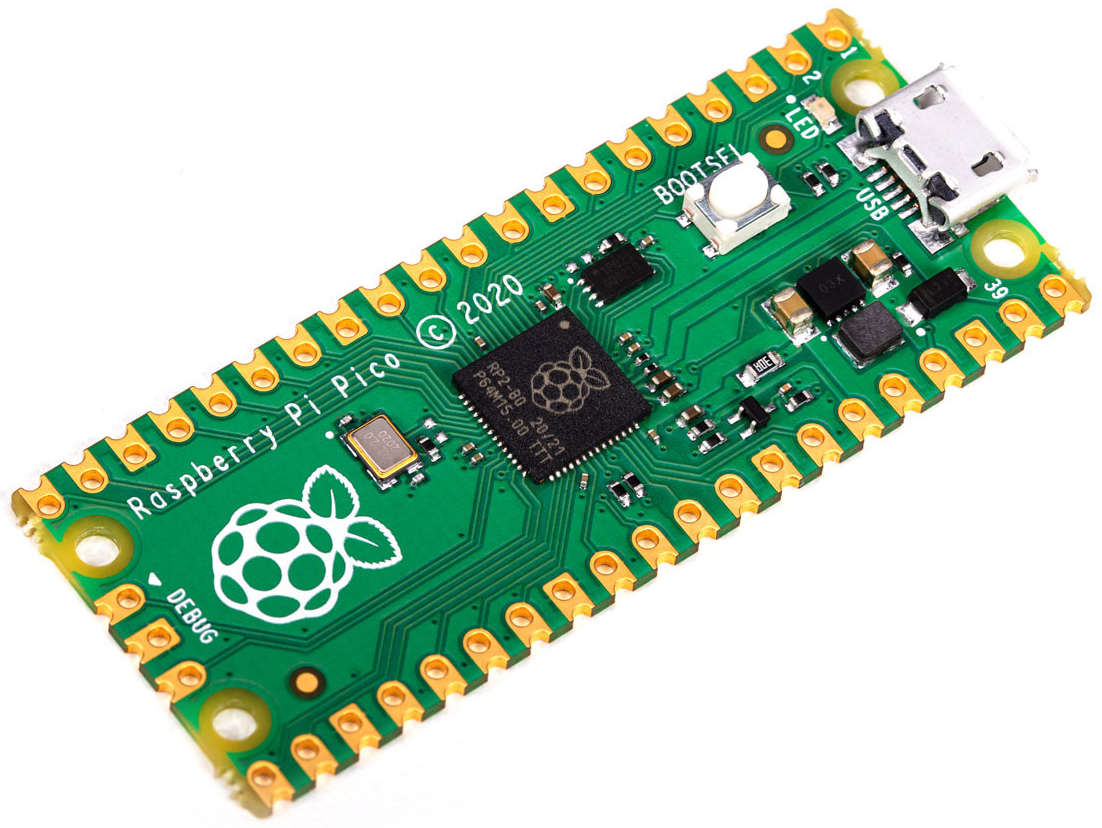
\includegraphics[scale=.1]{images/pico.jpg}}\quad
\subfloat[Proximity Sensor]{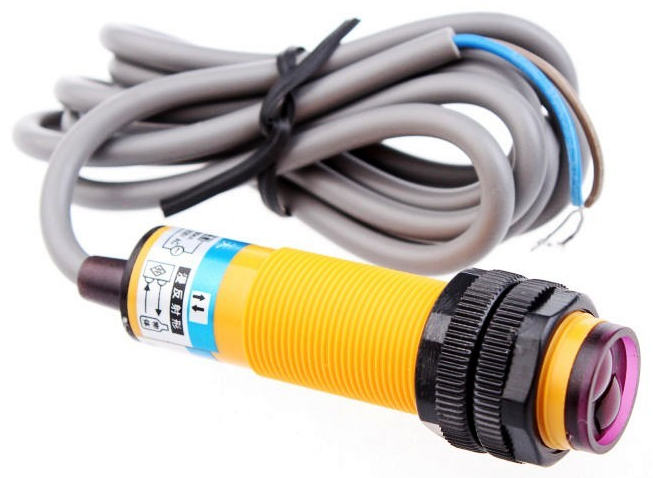
\includegraphics[scale=.12]{images/ir.jpg}}\quad
\subfloat[Four-digit 7-segment display]{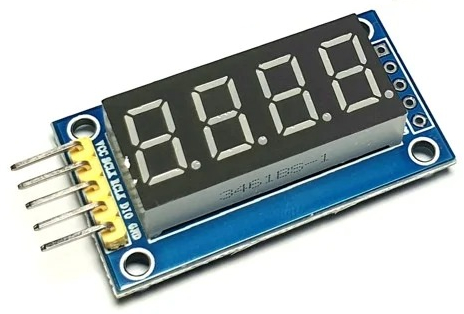
\includegraphics[scale=1]{images/7seg.jpg}}\quad
\subfloat[Buzzer]{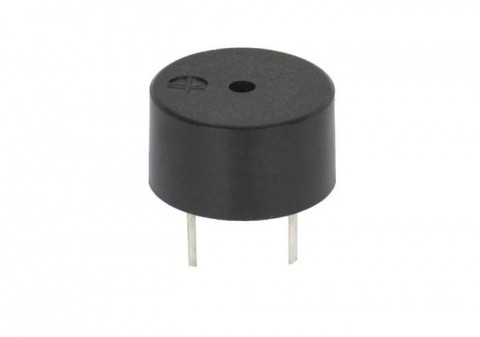
\includegraphics[scale=0.2]{images/buzzer.jpg}}
\caption{Used electrical components}
\end{figure}

The software would be written in C, using Keil-C and Pico device library \footfullcite{pico_mdk}. 

All resources will be open-sourced and uploaded on our GitHub repository. 

\chapter{Algorithm}
\section{Describe the algorithm}
This device counts the number of obstacles that pass in front of the IR sensor in one direction only. The value of the total counts or the count number is displayed on a four-digit 7-segment display module. The IR sensor that we are using in this project is an IR proximity sensor. Whenever it detects an object inside its range the output generated by it is high otherwise the output is low. The count is zero initially and then incremented by one whenever something passes in front of it.

\section{Flowchart}
\subsection{IO schematic}
\begin{figure}[H]
\centering
\begin{tikzpicture}
\node[inner sep=0pt] (pico) at (0,0)
    {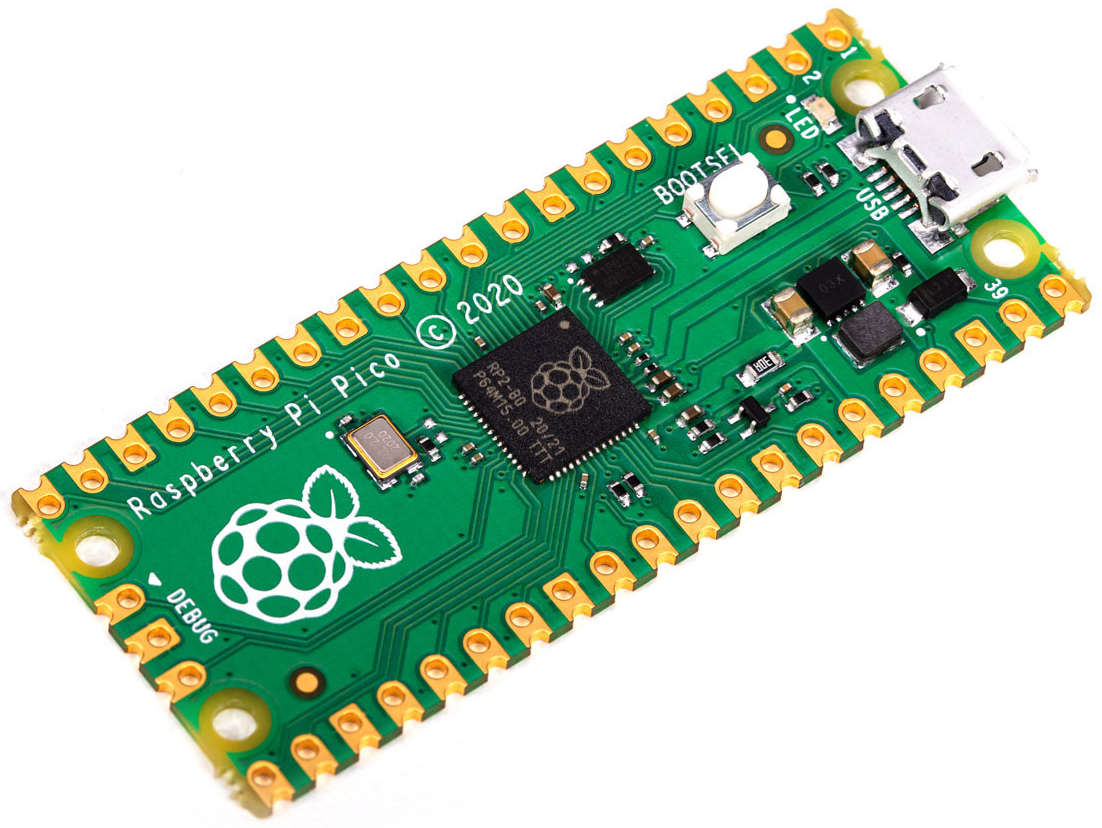
\includegraphics[scale=.125]{images/pico.jpg}};
    
\node[inner sep=0pt] (ir) at (7,3)
    {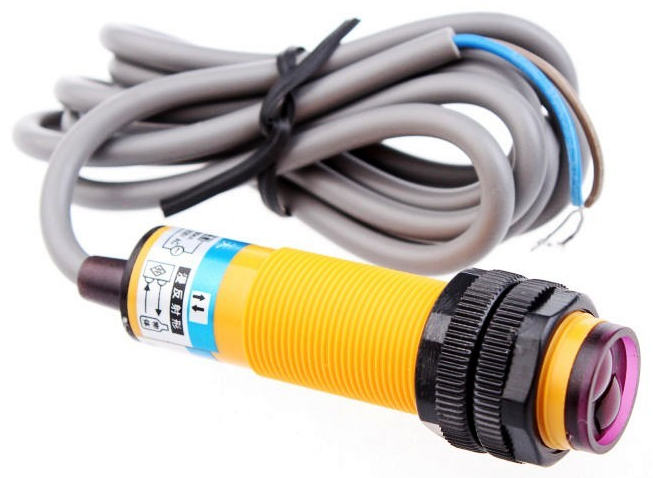
\includegraphics[scale=.175]{images/ir.jpg}};
    
\node[inner sep=0pt] (7seg) at (7,-3)
    {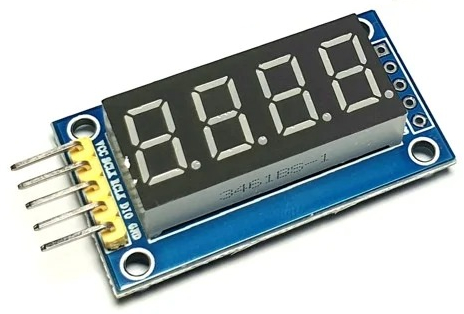
\includegraphics[scale=1]{images/7seg.jpg}};

\node[inner sep=0pt] (buzzer) at (7,-6)
    {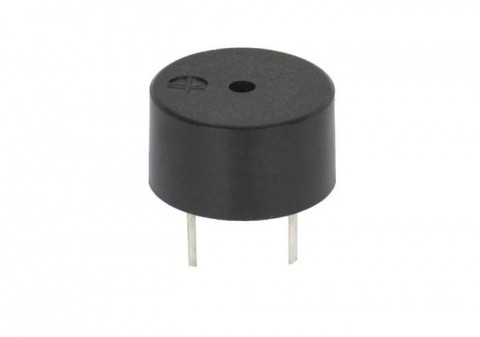
\includegraphics[scale=0.2]{images/buzzer.jpg}};
    
\draw [<-] (pico.north) |- (ir.west);
\draw [->] (pico.south) |- (7seg.west);
\draw [->] (pico.south) |- (buzzer.west);
\end{tikzpicture}
\end{figure}

\subsection{Method 1: program loop}
Using this method, the MCU will be constantly in a loop for reading IR, checking the IR state. The downside of this method is the program uses all CPU performance just for this simple task, wasting all of the power of the ARM Cortex M0+.
\subsubsection{Finite State Machine}
\begin{figure}[H]
\centering
\begin{tikzpicture}
\tikzset{
->, % makes the edges directed
node distance=3.8cm, % specifies the minimum distance between two nodes. Change if necessary.
every state/.style={thick, fill=gray!10}, % sets the properties for each ’state’ node
initial text=$ $, % sets the text that appears on the start arrow
}
\node[state] (start) {Start};
\node[state, right of=start] (readir) {Read IR};
\node[state, right of=readir] (inc_counter) {\makecell{Increase\\counter}};
\node[state, right of=inc_counter] (readir2) {Read IR};

\draw
(start) edge[above] (readir)
(readir) edge[loop above] node{$0$} (readir)
(readir) edge[above] node[above] {$1$} (inc_counter)
(inc_counter) edge[above] (readir2)
(readir2) edge[loop above] node{$1$} (readir2)

(readir2) edge[bend left, below] node[]{$0$} (readir)
;

\end{tikzpicture}
\end{figure}

\subsubsection{Program Flow}
		\begin{figure}[H]
			\centering
			\begin{tikzpicture}[node distance=1cm and 1cm,auto]
				\node (init) [startstop] {Start};
				\node (readir) [process, below =of init] {Read IR state};
				\node (obj_found) [decision, below =of readir] {Object Found?};
				\node (inc_counter) [process, below =of obj_found] {\makecell{Increase counter\\Update display}};
				\node (readir2) [process, below =of inc_counter] {Read IR state};
				\node (obj_found2) [decision, below =of readir2] {Object Found?};
				
				
				
				\draw [arrow] (init) -- (readir);
				\draw [arrow] (readir) -- (obj_found);
				\draw [arrow] (obj_found) -- node[anchor=west] {true}(inc_counter);
				\draw [arrow] (obj_found) -- +(3,0) node[anchor=south east] {false} |- (readir);
				\draw [arrow] (inc_counter) -- (readir2);
				\draw [arrow] (readir2) -- (obj_found2);
				\draw [arrow] (obj_found2) -- +(3,0) node[anchor=south east] {true} |- (readir2);
				\draw [arrow] (obj_found2) -- +(-3,0) node[anchor=south west] {false} |- (readir);
				
				
			\end{tikzpicture}
			\label{fig:flowchart}
		\end{figure}
		
\subsubsection{Pseudo Code}
\begin{minted}[escapeinside=||,mathescape=true, baselinestretch=0.8]{text}
|\textcolor{red}{LOOP}|:
    COUNT := 0
    IR := ReadIR()
    |\textcolor{blue}{IF}| (IR == HIGH) |\textcolor{blue}{THEN}|
        COUNT++
        UPDATE 7-segment display
        IR = ReadIR()
        |\textcolor{blue}{WHILE}| (IR == HIGH) |\textcolor{blue}{DO}|
            IR = ReadIR()
        |\textcolor{blue}{END WHILE}|
        |\textcolor{blue}{GOTO}| LOOP
    |\textcolor{blue}{END IF}|
    |\textcolor{blue}{GOTO}| LOOP
\end{minted}

\subsection{Method 2: using interrupt}
By using this method, the counter increment will just process when there is interruption of the proximity sensor, leaving all CPU free for other heavy tasks when there is no object detected.
\subsubsection{Program Flow}

		\begin{figure}[H]
			\centering
			\subfloat[(a) Main program]{
			\begin{tikzpicture}[node distance=1cm and 1cm,auto]
				\node (start) [startstop] {Start};
				\node (init) [process, below =of start] {\makecell{Initialization\\(setup interrupt)}};
				\node (otherprocess) [process, below =of init] {Other tasks/loop};
				\node (stop) [startstop, below =of otherprocess] {Stop};
				
				\draw [arrow] (start) -- (init);
				\draw [arrow] (init) -- (otherprocess);
				\draw [arrow] (otherprocess) -- (stop);
				
			\end{tikzpicture}
			} \qquad \qquad
			\subfloat[(b) Sensor ISR]{
			\begin{tikzpicture}[node distance=1cm and 1cm,auto]
				\node (start) [startstop] {\makecell{ISR of IR\\(invoke when falling edge)}};
				\node (inc_counter) [process, below =of start] {\makecell{Increase counter\\Update display}};
				\node (stop) [startstop, below =of inc_counter] {Exit ISR};
				
				\draw [arrow] (start) -- (inc_counter);
				\draw [arrow] (inc_counter) -- (stop);
				
			\end{tikzpicture}
			}
		\end{figure}
		
\subsubsection{Pseudo Code}
\begin{minted}[escapeinside=||,mathescape=true, baselinestretch=0.8]{text}
|\textcolor{red}{MAIN PROGRAM}|:
    INIT_ISR
    COUNT := 0
    DO TASKS / LOOPS
|\textcolor{red}{END PROGRAM}|

|\textcolor{red}{IR\_ISR}|:
    COUNT++
    UPDATE 7-segment display
|\textcolor{red}{END IR\_ISR}|
\end{minted}

\chapter{Hardware}
\section{Raspberry Pi Pico}
Raspberry Pi Pico is a low-cost, high-performance microcontroller board with flexible digital interfaces. It incorporates Raspberry Pi's own RP2040 microcontroller chip, with a dual-core ARM Cortex M0+ processor running up to 133 MHz, embedded 264KB of SRAM, 2MB of onboard Flash memory, as well as 26 × multi-function GPIO pins.

For software development, either Raspberry Pi's C/C++ SDK or the MicroPython is available. In this project, we will use Raspberry Pi's C/C++ SDK, along with Gabriel Wang's Pico Template to use with Keil C.

\subsubsection{Features}
\begin{itemize}
\item RP2040 microcontroller chip designed by Raspberry Pi in the United Kingdom.
\item Dual-core Arm Cortex M0+ processor, the flexible clock running up to 133 MHz.
\item 264KB of SRAM, and 2MB of onboard Flash memory.
\item USB 1.1 with device and host support.
\item Low-power sleep and dormant modes.
\item 26 × multi-function GPIO pins.
\item 2 × SPI, 2 × I2C, 2 × UART, 3 × 12-bit ADC, 16 × controllable PWM channels.
\item Accurate clock and timer on-chip.
\item Temperature sensor.
\item Accelerated floating-point libraries on-chip.
\item 8 × Programmable I/O (PIO) state machines for custom peripheral support.
\end{itemize}

\begin{figure}[H]
\centering
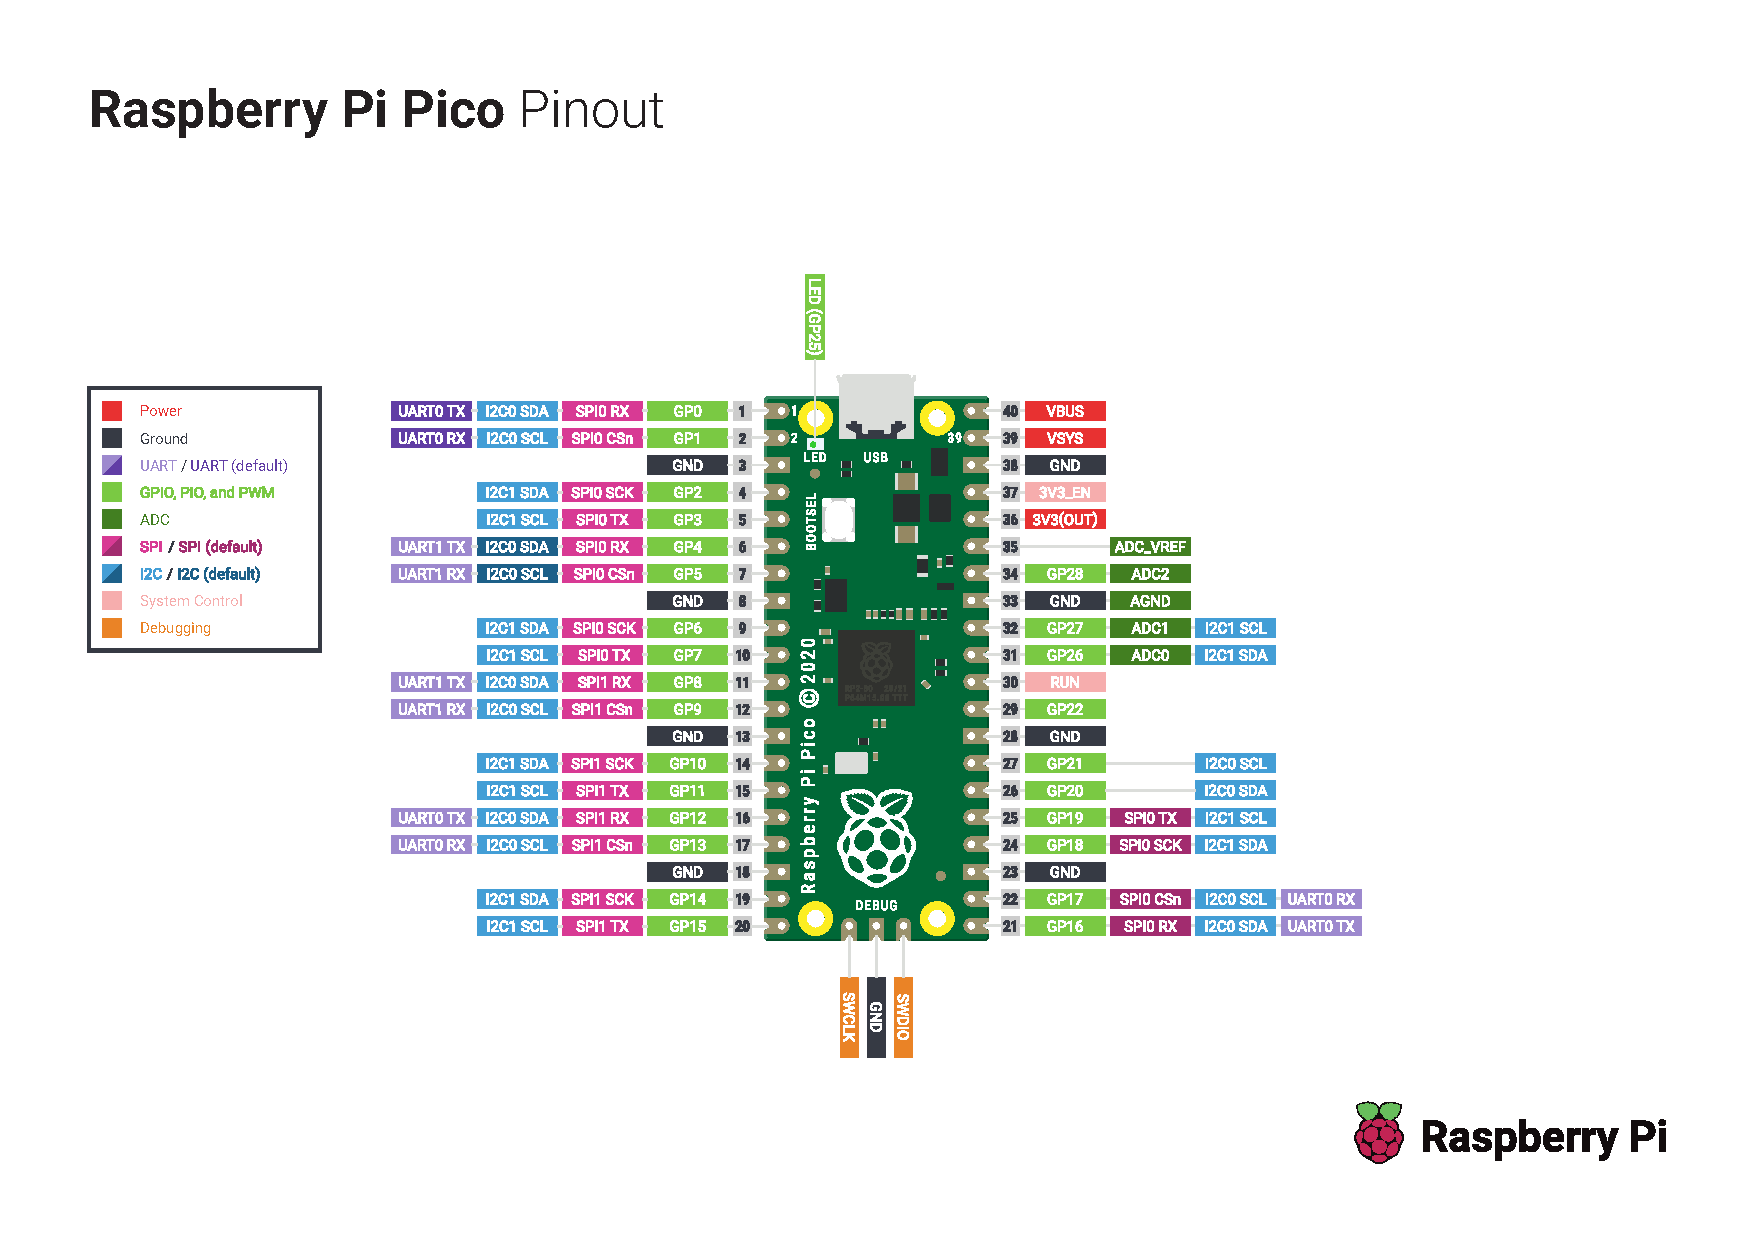
\includegraphics[scale=0.5, trim={0cm, 3cm, 0cm, 5cm},clip]{images/Pico-R3-A4-Pinout.pdf}
\caption{Raspberry Pi Pico pinout diagram\protect\footnotemark}
\end{figure}

\footnotetext{\fullcite{pico_pinout}}

\section{Infrared Proximity Sensor}
An infrared sensor is an electronic device, that emits in order to sense some aspects of the surroundings. An IR sensor can measure the heat of an object as well as detects the motion. These types of sensors measure only infrared radiation, rather than emitting it that is called a passive IR sensor. Usually, in the infrared spectrum, all the objects radiate some form of thermal radiation.

These types of radiations are invisible to our eyes, which can be detected by an infrared sensor. The emitter is simply an IR LED (Light Emitting Diode) and the detector is simply an IR photodiode that is sensitive to IR light of the same wavelength as that emitted by the IR LED. When IR light falls on the photodiode, the resistances and the output voltages will change in proportion to the magnitude of the IR light received.

There are two IR LED in an IR sensor:
\begin{itemize}
\item Infrared Transmitter: an LED which emits infrared radiations. Even though an IR LED looks like a normal LED, the radiation emitted by it is invisible to the human eye.
\item Infrared receivers or infrared sensors: detect the radiation from an IR transmitter. IR receivers come in the form of photodiodes and phototransistors. Infrared Photodiodes are different from normal photo diodes as they detect only infrared radiation.
\end{itemize}

\begin{figure}[H]
\centering
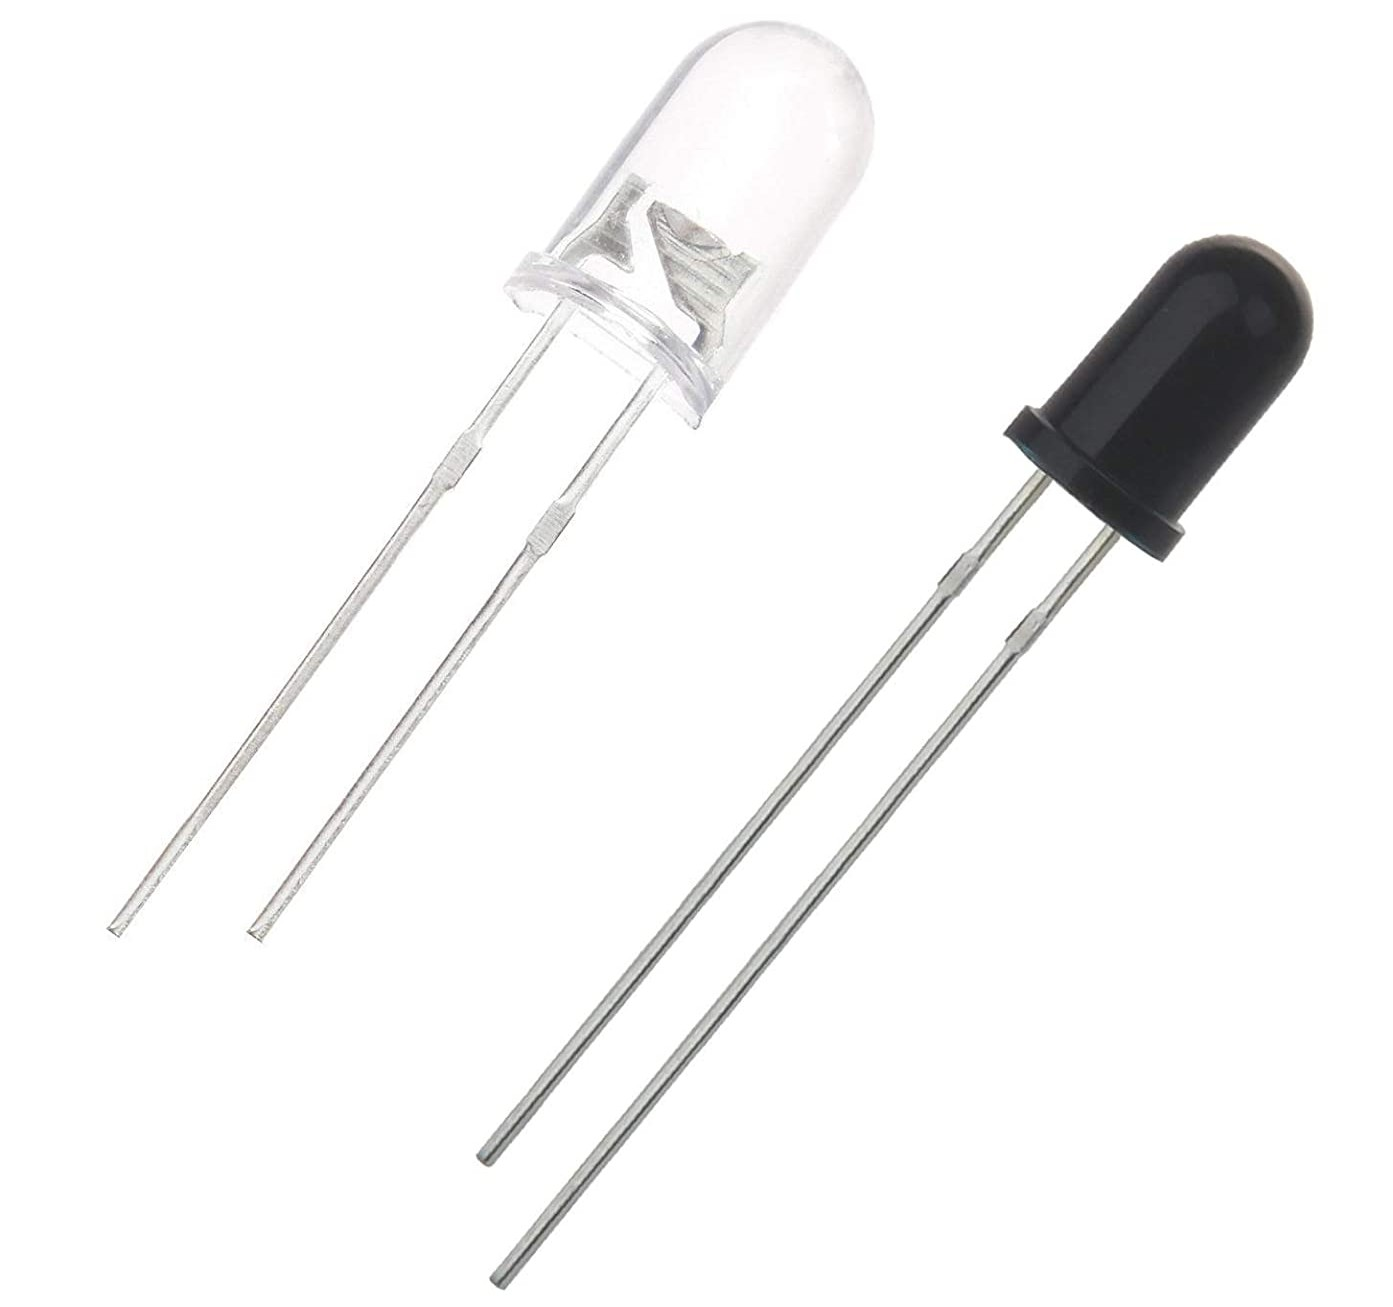
\includegraphics[scale=0.09]{images/ir_trans_recev.jpg}
\caption{IR transmitter (left) and IR receiver (right)}
\end{figure}

When the IR transmitter emits radiation, it reaches the object and some of the radiation reflects back to the IR receiver. Based on the intensity of the reception by the IR receiver, the output of the sensor defines.
\begin{figure}[H]
\centering
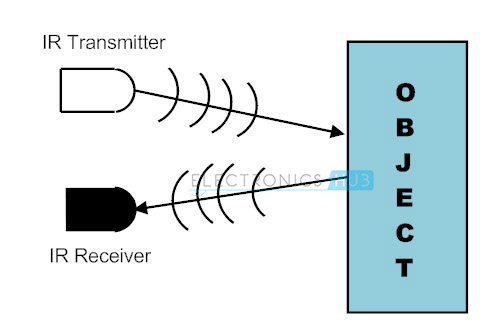
\includegraphics[scale=0.5]{images/ir_principle.jpg}
\caption{Infrared sensor working principle\protect\footnotemark}
\end{figure}

\footnotetext{\fullcite{ir_working}}

In this project, we will be using an E3F-DS30C4 Adjustable IR Infrared Proximity Sensor.

\begin{figure}[H]
\centering
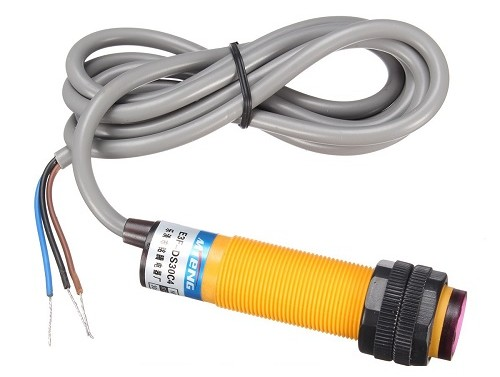
\includegraphics[scale=0.4]{images/prox_sensor.jpg}
\caption{E3F-DS30C4 Adjustable IR Infrared Proximity Sensor}
\end{figure}

E3F-DS30C4 Adjustable IR Infrared Proximity Sensor provides a good distance measuring (5 to 30 cm), power supply reversal connection protection, short-circuit protection, a small potentiometer to adjust sensitivity and more. But the most significant feature is signal interference prevention, best for detecting moving objects. There are three wires on the sensor:
\begin{itemize}
\item Brown: Power source (5 to 36 V)
\item Blue: Ground
\item Black: Signal output, the sensor is normally open (active low), so when the sensor detect objects, the output signal will be low.
\end{itemize}

\section{Four-digit 7-segment display with built-in shift registers}
\subsection{7-segment display}
A seven-segment display is a form of electronic display device for displaying decimal numerals. As the name stated, the device uses seven segment (denoted from a to g) to display a number or a character in alphabet. Some device even contains a decimal point segment (denoted as p or dp). \cite{wiki:7seg}
\begin{figure}[H]
\centering
\def\svgwidth{.17\textwidth}
\input{images/7-seg-labeled.pdf_tex}
\caption{7-segment display segments naming}
\end{figure}

Every segment is represented by one-bit value, 1/0 (active high) or 0/1 (active low) for on/off. Here is a table for binary and hexadecimal encoding for displaying 0 to F.

\newcommand{\led}[1]{
\begin{circuitikz}
	\ctikzset{seven seg/width=0.2, seven seg/thickness=2pt}
	\draw (0,0) node[seven segment val=#1 dot off box off]{};
\end{circuitikz}
}
\begin{table}[H]
\centering
\caption{Binary and hexadecimal encoding for displaying 0 to F}
\begin{tabular}{|c|c|c|c|c|c|c|c|c|c|c|c|c|c|}
\hline
Digit & Display & p & a & b & c & d & e & f & g & abcdefg & hex pabcdefg & \textoverline{pgfedcba} & hex \textoverline{pabcdefg}\\\hline
0 & \led{0} & 0 & 1 & 1 & 1 & 1 & 1 & 1 & 0 & 01111110 & 0x7E & 11000000 & 0xC0\\\hline
1 & \led{1} & 0 & 0 & 1 & 1 & 0 & 0 & 0 & 0 & 00110000 & 0x30 & 11111001 & 0xF9\\\hline
2 & \led{2} & 0 & 1 & 1 & 0 & 1 & 1 & 0 & 1 & 01101101 & 0x6D & 10100100 & 0xA4\\\hline
3 & \led{3} & 0 & 1 & 1 & 1 & 1 & 0 & 0 & 1 & 01111001 & 0x79 & 10110001 & 0xB0\\\hline
4 & \led{4} & 0 & 0 & 1 & 1 & 0 & 0 & 1 & 1 & 00110011 & 0x33 & 10011001 & 0x99\\\hline
5 & \led{5} & 0 & 1 & 0 & 1 & 1 & 0 & 1 & 1 & 01011011 & 0x5B & 10010010 & 0x92\\\hline
6 & \led{6} & 0 & 1 & 0 & 1 & 1 & 1 & 1 & 1 & 01011111 & 0x5F & 10000010 & 0x82\\\hline
7 & \led{7} & 0 & 1 & 1 & 1 & 0 & 0 & 0 & 0 & 01110000 & 0x70 & 11111000 & 0xF8\\\hline
8 & \led{8} & 0 & 1 & 1 & 1 & 1 & 1 & 1 & 1 & 01111111 & 0x7F & 10000000 & 0x80\\\hline
9 & \led{9} & 0 & 1 & 1 & 1 & 1 & 0 & 1 & 1 & 01111011 & 0x7B & 10010000 & 0x90\\\hline
A & \led{A} & 0 & 1 & 1 & 1 & 0 & 1 & 1 & 1 & 01110111 & 0x77 & 10001000 & 0x8C\\\hline
b & \led{b} & 0 & 0 & 0 & 1 & 1 & 1 & 1 & 1 & 00011111 & 0x1F & 10000011 & 0xBF\\\hline
C & \led{C} & 0 & 1 & 0 & 0 & 1 & 1 & 1 & 0 & 01001110 & 0x4E & 11000110 & 0xC6\\\hline
d & \led{d} & 0 & 0 & 1 & 1 & 1 & 1 & 0 & 1 & 00111101 & 0x3D & 10100001 & 0xA1\\\hline
E & \led{E} & 0 & 1 & 0 & 0 & 1 & 1 & 1 & 1 & 01001111 & 0x4F & 10000110 & 0x86\\\hline
F & \led{F} & 0 & 1 & 0 & 0 & 0 & 1 & 1 & 1 & 01000111 & 0x47 & 10001110 & 0x8E\\\hline
- & \led{-} & 0 & 0 & 0 & 0 & 0 & 0 & 0 & 1 & 00000001 & 0x01 & 10111111 & 0xBF\\\hline
off & \led{} & 0 & 0 & 0 & 0 & 0 & 0 & 0 & 0 & 00000000 & 0x00 & 11111111 & 0xFF\\\hline

\end{tabular}
\end{table}

\subsection{Multiplexed display}
Multiplexed displays are basically multiple displays which are multiplexed together and usually one is turned on at a time, the turning on and off of multiple displays are so fast that viewer is able to believe that all the displays are turned on at a time. \cite{multiplex_7seg}
 
Multiplexing of displays have some benefits like reduced number of input pins, reduced complexity and less power is required for the display. In this project we will use 4-digit 7-segment multiplexed display. If we use 4 different one-digit 7-segment (with decimal point) display, we need $9\times 4=36$ pins. On this multiplexed display, we only need $8 + 4=12$ pins only. 

\begin{figure}[H]
\centering
\subfloat[Front view and pinout]{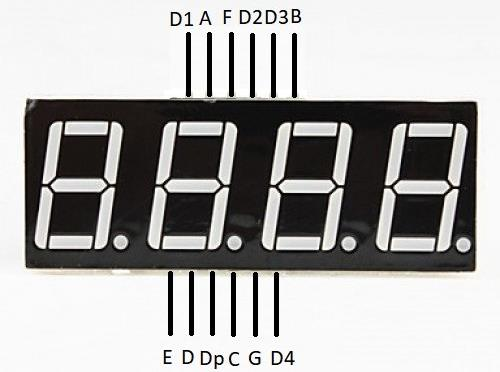
\includegraphics[scale=0.3]{images/4-digit_7-seg.jpg}}\\
\subfloat[Schematic]{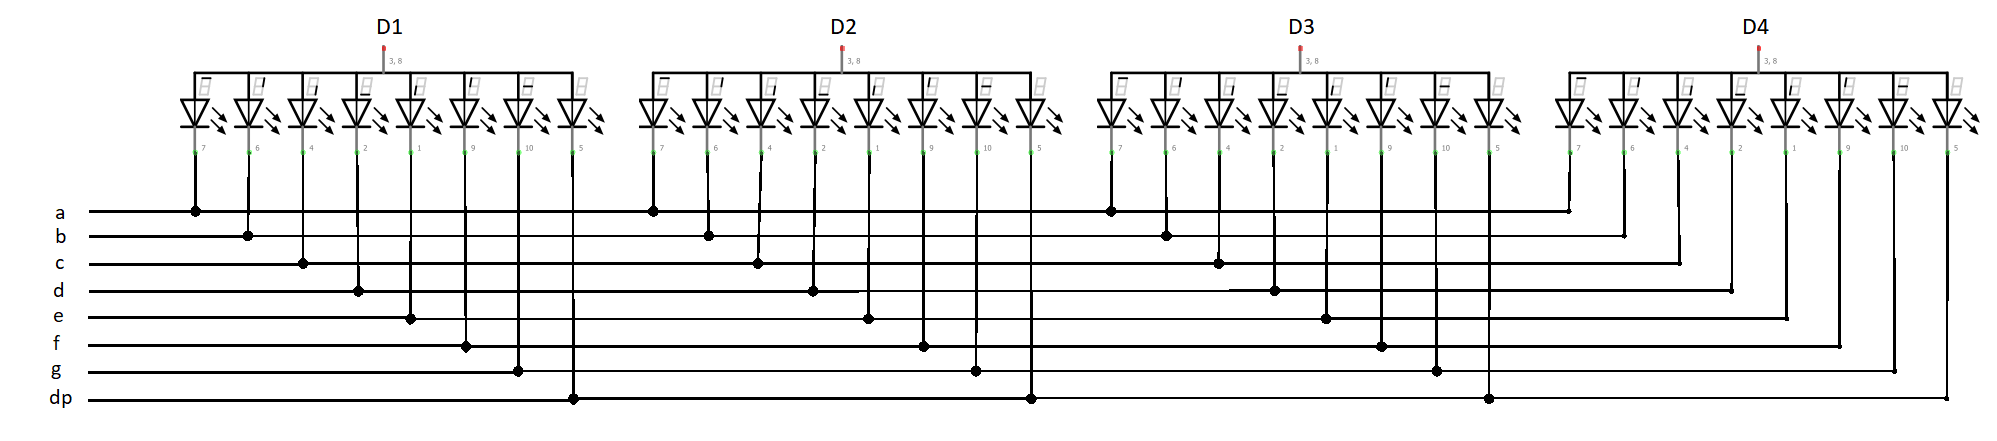
\includegraphics[scale=0.45]{images/4-digit_7-seg_sche.png}}
\caption{Four-digit 7-segment display\protect\footnotemark}
\end{figure}

\footnotetext{\fullcite{multiplex_7seg}}

To turn on a segment, output high to desired the digit (\texttt{D1}, \texttt{D2}, \texttt{D3} or \texttt{D4}) and output low to the disired segment (\texttt{a}, \texttt{b}, \texttt{c}, \texttt{d}, \texttt{e}, \texttt{f}, \texttt{g}). The current flows from high potential to low potential to light up the segment.

Assume we want to display 1111, it is easy as we can give output high to \texttt{D1}, \texttt{D2}, \texttt{D3}, \texttt{D4} (4 columns to turn on all 4  digits) and low to b, c (segment b and c is to drive number 1 on a seven segment). But in case we want to display 1234, it can not be easy to do, if we drive 1 using segments then all the digits will display 1 since there is no separate segment pins for each individual digit.

Solution to this problem is making use of multiplexing, first output high to \texttt{D1} and output low to all other digits and display 1, then output high to \texttt{D2} and output low to all other digits and display 2, same goes for \texttt{D3} and \texttt{D4} and we start this over. When interval between turning high and turning low is few milliseconds, a human eye will not be able to see any blinking and viewer will feel all the digits are on at a time.

\subsection{Shift register 74HC595}
TM74HC595 is an open-drain output CMOS shift register which is designed with controllable tri-state output terminals and, when in serial output configuration, can control cascade chip of next stage. This product is excellent in performance and reliable in quality.

The 74HC595 is capable of handling high-speed shift clock frequency $(F_{\text{max}} > 25 \text{MHz})$, Standard SPI, CMOS serial output and capable of cascading multiple devices. This device can be treated as a serial-to-paralell data converter.

The schematic below will explain how the IC works.

\begin{figure}[H]
\centering
\subfloat[Pinout]{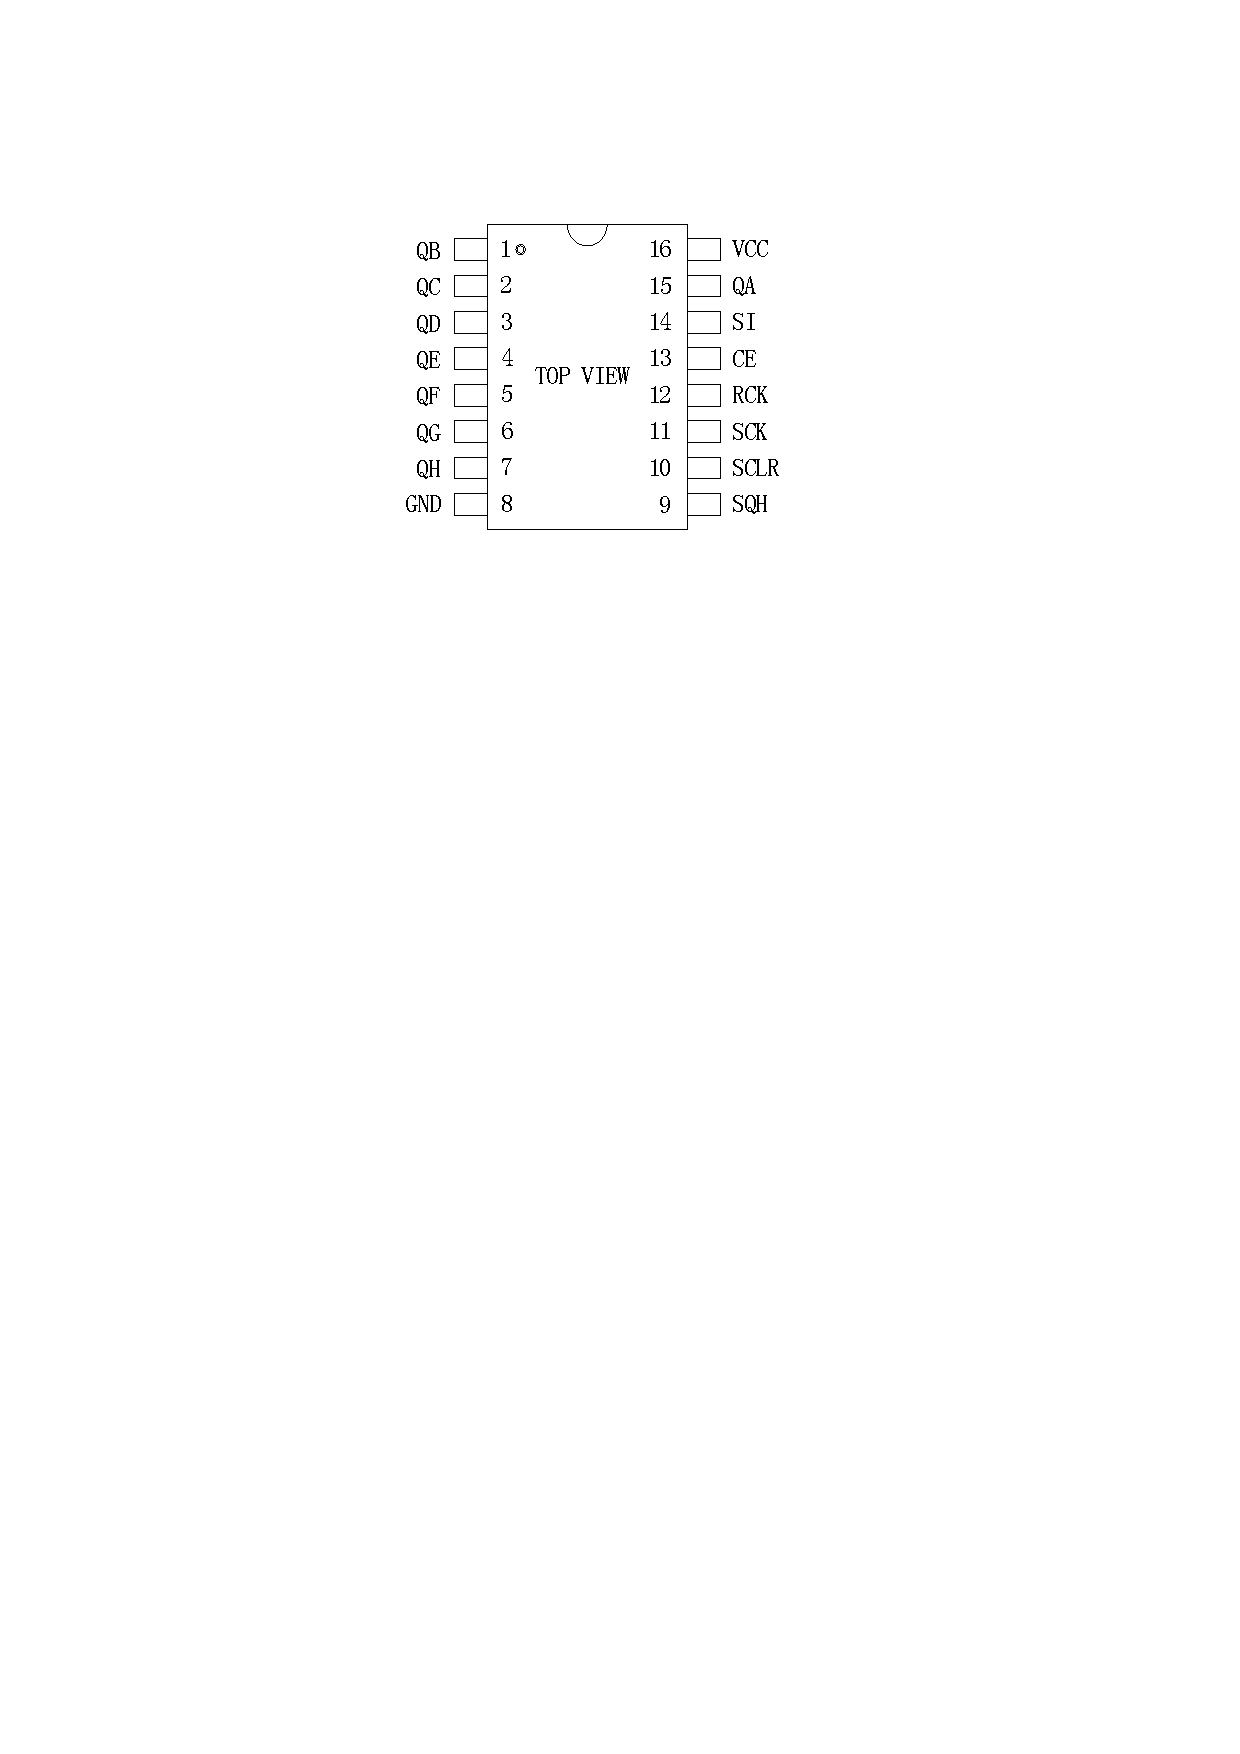
\includegraphics[scale=0.6]{images/tm74hc595_ic.pdf}}\\
\subfloat[Schematic]{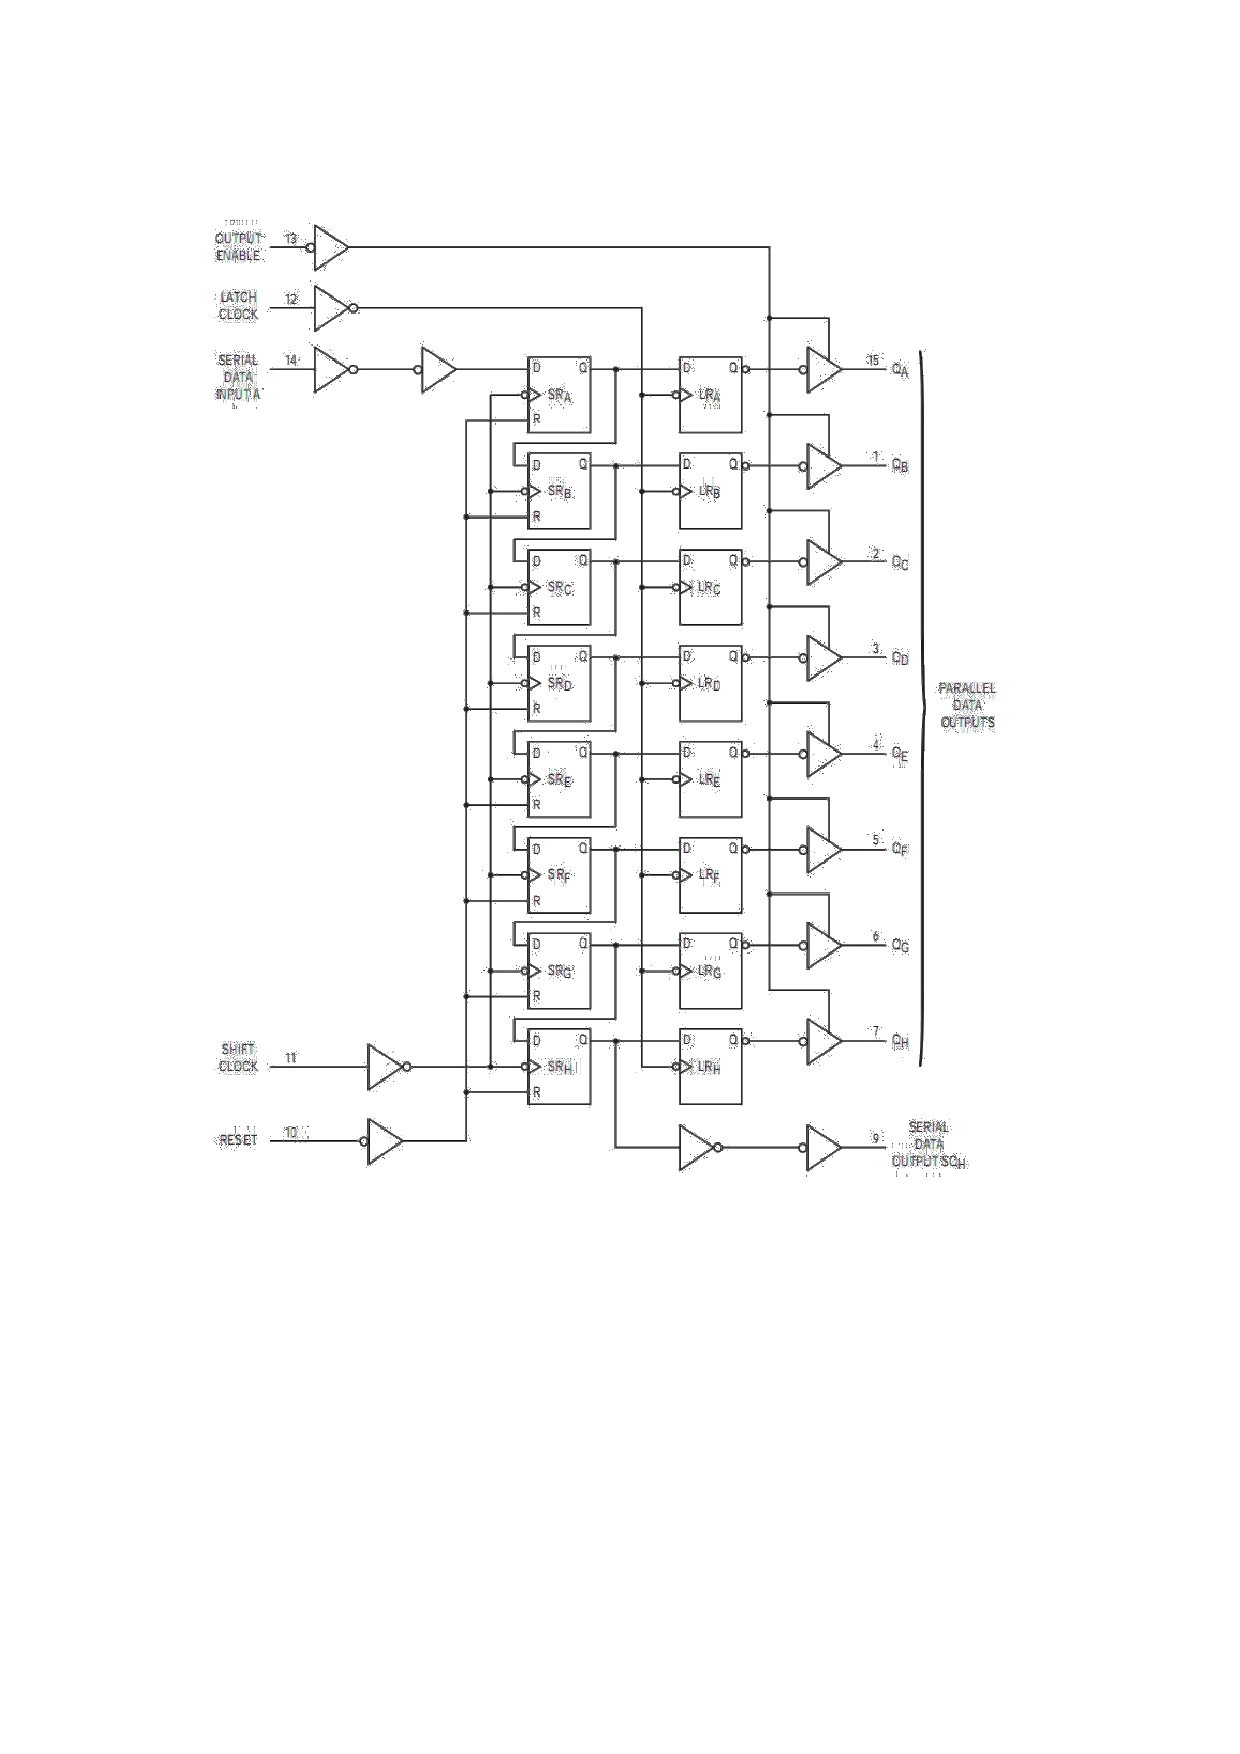
\includegraphics[scale=0.8]{images/tm74hc595_schem.pdf}}
\caption{TM74HC595 shift register IC\protect\footnotemark}
\end{figure}

\footnotetext{\fullcite{shiftreg_datasheet}}

\subsection{Multiplexed Display with 74HC595}
\begin{figure}[H]
\centering
\subfloat[Front view]{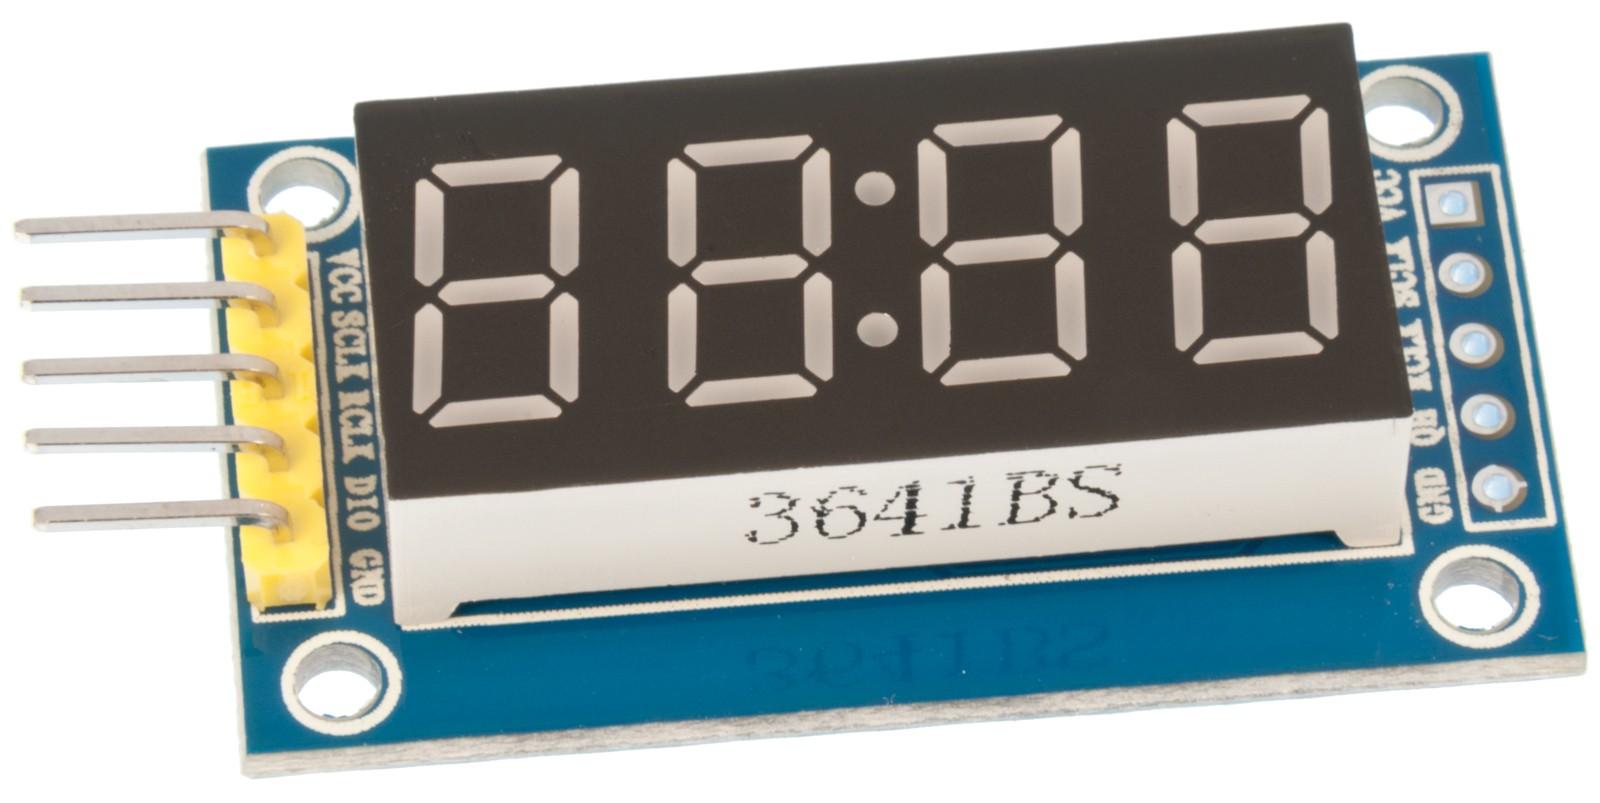
\includegraphics[width=.28\textwidth]{images/7seg_front.jpg}}\qquad\qquad
\subfloat[Back view]{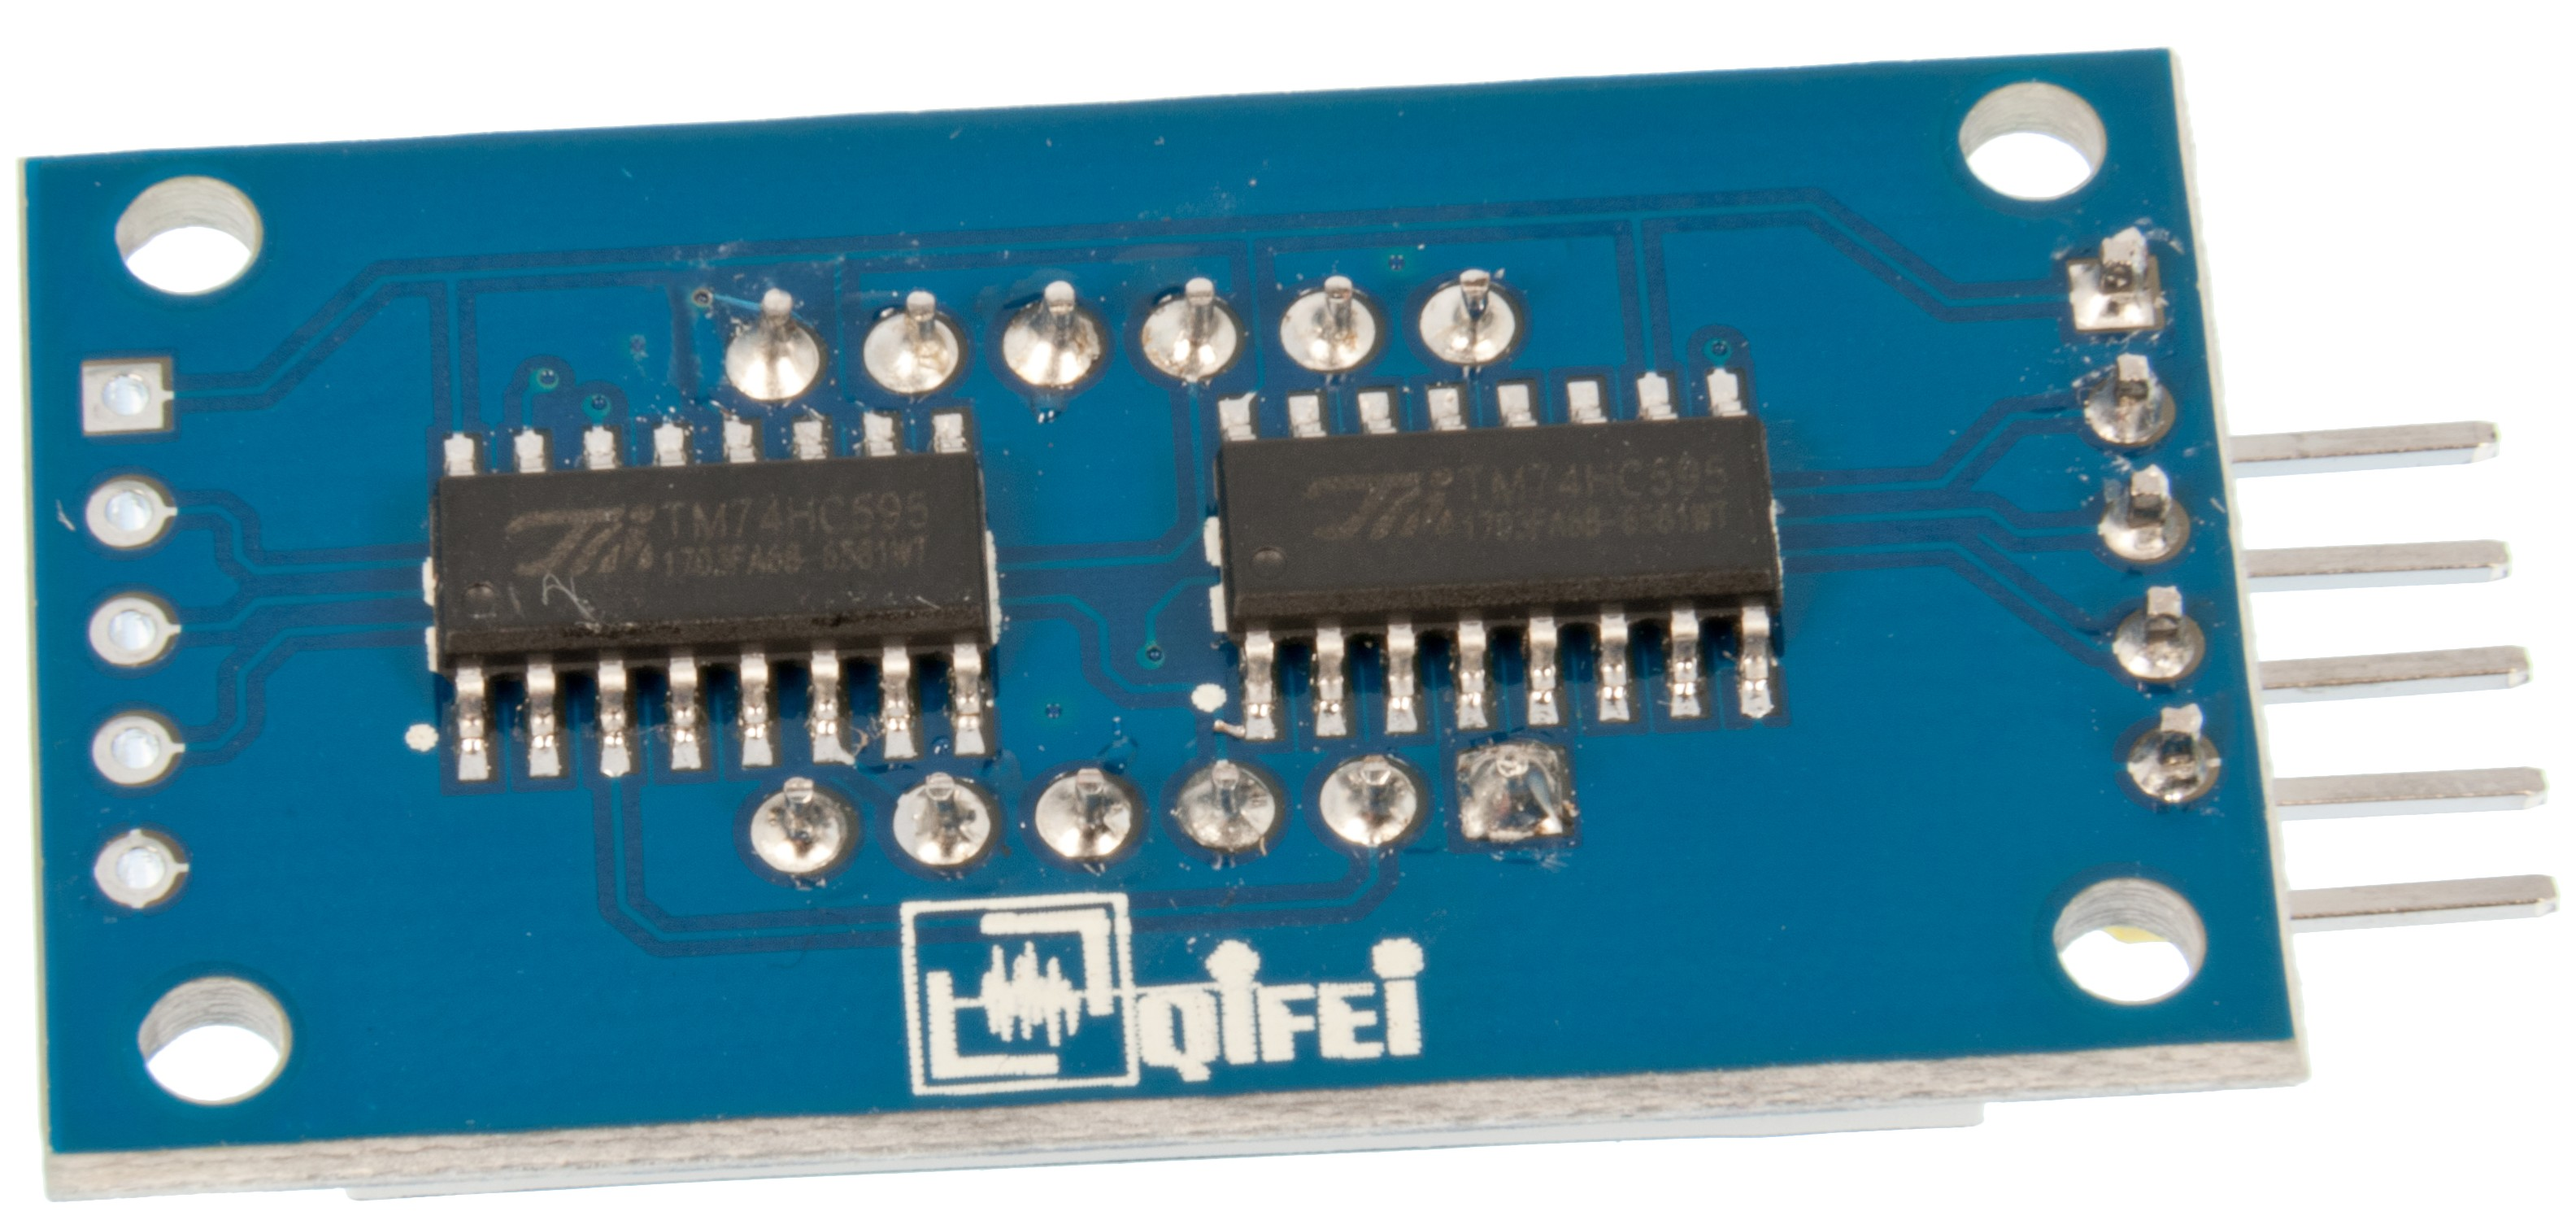
\includegraphics[width=.28\textwidth]{images/7seg_back.jpg}}
\caption{Four-digit 7-segment display with 74HC595 module}
\end{figure}

\begin{figure}[H]
\centering
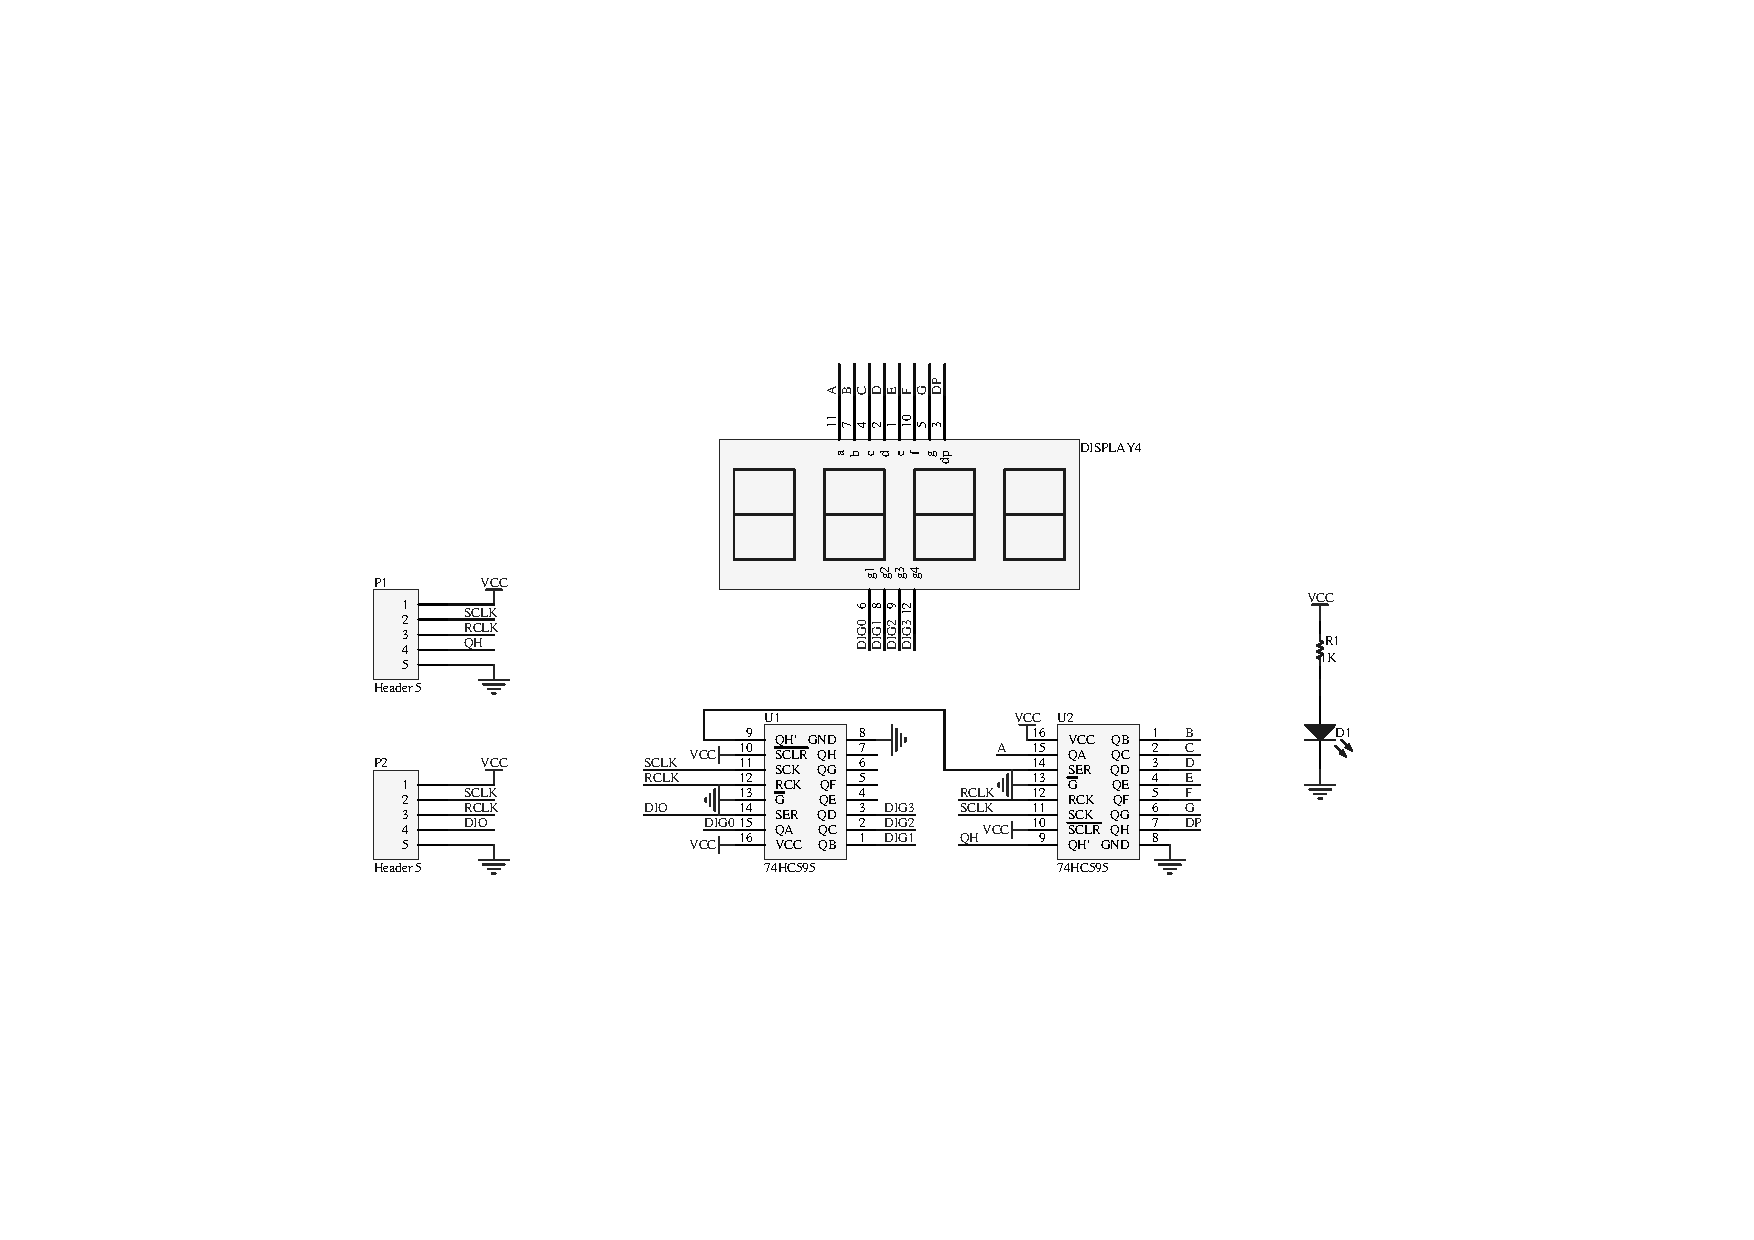
\includegraphics[scale=0.82]{images/7seg_module_schem.pdf}
\caption{Four-digit 7-segment display with 74HC595 module schematic}
\end{figure}

Module pinout:
\begin{multicols}{2}
\begin{itemize}
\item \texttt{VCC}: Power source
\item \texttt{SCLK}: Shift clock
\item \texttt{RCLK}: Latch clock
\item \texttt{DIO}: Serial data input
\item \texttt{QH}: Serial data output
\item \texttt{GND}: Ground
\end{itemize}
\end{multicols}
According to the schematic, the module contains two 74HC595s. The first one drives the signal for \texttt{D1}, \texttt{D2}, \texttt{D3} and \texttt{D4}. The second one drives the signal for the segments. 

\texttt{SCLK} and \texttt{RCLK} will in turn provide the clock for the flip flop in the active 7-segment display. Specifically, \texttt{SCLK} helps to temporarily store the value of the number that needs to be released next, while \texttt{RCLK} will perform to update the display output of 7-segment display.

For example, to show 1234 on the display, according to the table above, the data is \texttt{F9 A4 B0 99 = 11111001 10100100 10110001 10011001}, respectively. Here is the data sequence need to be sent:

\begin{multicols}{2}
\begin{itemize}
\item Send the \nth{1} digit data: 11111001.
\item Send 1000 to enable \texttt{D1}.

\item Send the \nth{2} digit data: 10100100.
\item Send 1000 to enable \texttt{D2}.

\item Send the \nth{3} digit data: 10110001.
\item Send 1000 to enable \texttt{D3}.

\item Send the \nth{4} digit data: 10011001.
\item Send 1000 to enable \texttt{D4}.
\end{itemize}
\end{multicols}

\section{Buzzer}
A buzzer or beeper is an audio signaling device, which may be mechanical, electromechanical, or piezoelectric. Typical uses of buzzers and beepers include alarm devices, timers, train and confirmation of user input such as a mouse click or keystroke.

A typical buzzer has two wire: anode (+) and cathode ($-$). The buzzer usually makes use of a material that has piezoelectric properties. When a material is piezoelectric, it means that applying mechanical force will cause it to gain charge. Inversely, applying an electric charge will cause the material to stretch or expand a very small amount. By pulsing our buzzer on and off we make the piezoelectric material inside quickly expand and contract. This produces the vibrations we hear in the air. So, in order to make it works, apply 5V to anode and ground to cathode.

\begin{figure}[H]
\centering
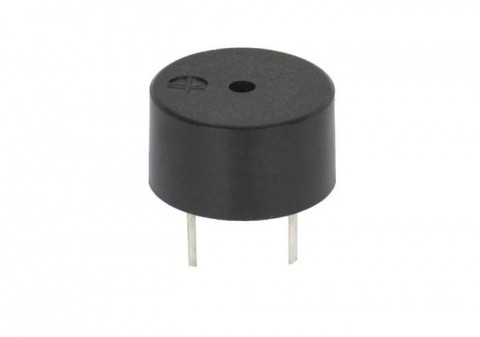
\includegraphics[scale=0.2]{images/buzzer.jpg}
\caption{A buzzer}
\end{figure}

\section{Wiring schematic}
The schematic is drawn using Fritzing\footnote{Fritzing is an open-source electronics design and prototyping platform for makers, hobbyists, and educators.}. A larger figure will be placed at Appendix section.
\begin{figure}[H]
\centering
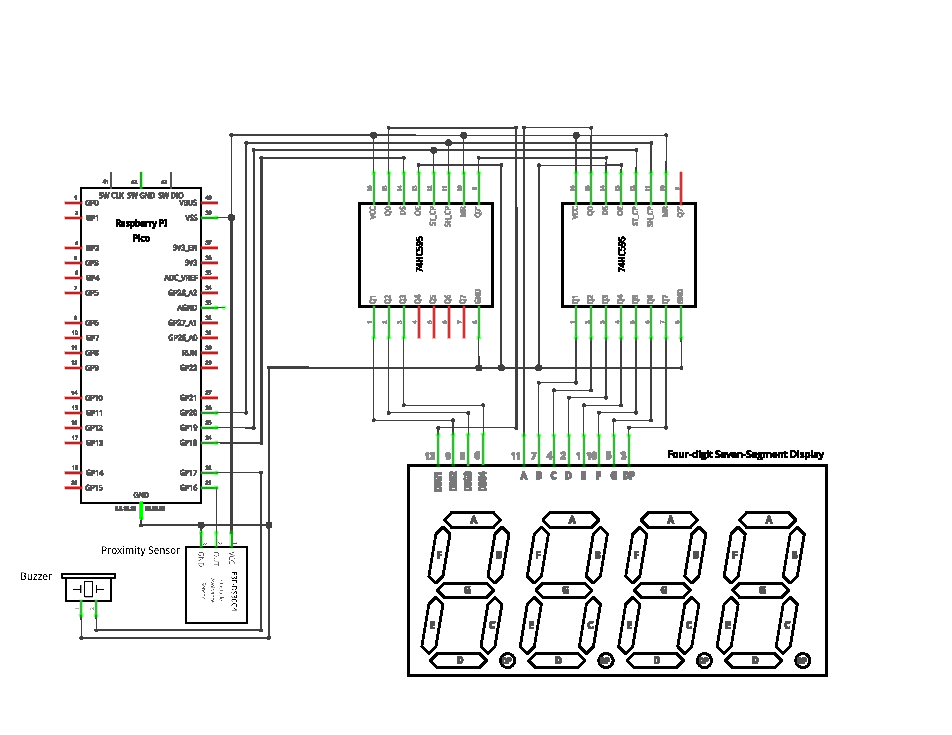
\includegraphics[scale=0.7,angle=0]{images/wiring_schem.pdf}
\caption{Overall wiring schematic}
\end{figure}

\section{3D Printed Case}
To finish the hardware part, we use Autodesk Fusion 360 to design a 3D printed case for making the device more compact and portable. A rectangular hole at the top for four-digit 7-segment display. A circular and rectangular holes at two sides for proximity sensor and micro USB port. A detail CAD schematic with dimentions is presented in Appendix section.

\begin{figure}[H]
\centering
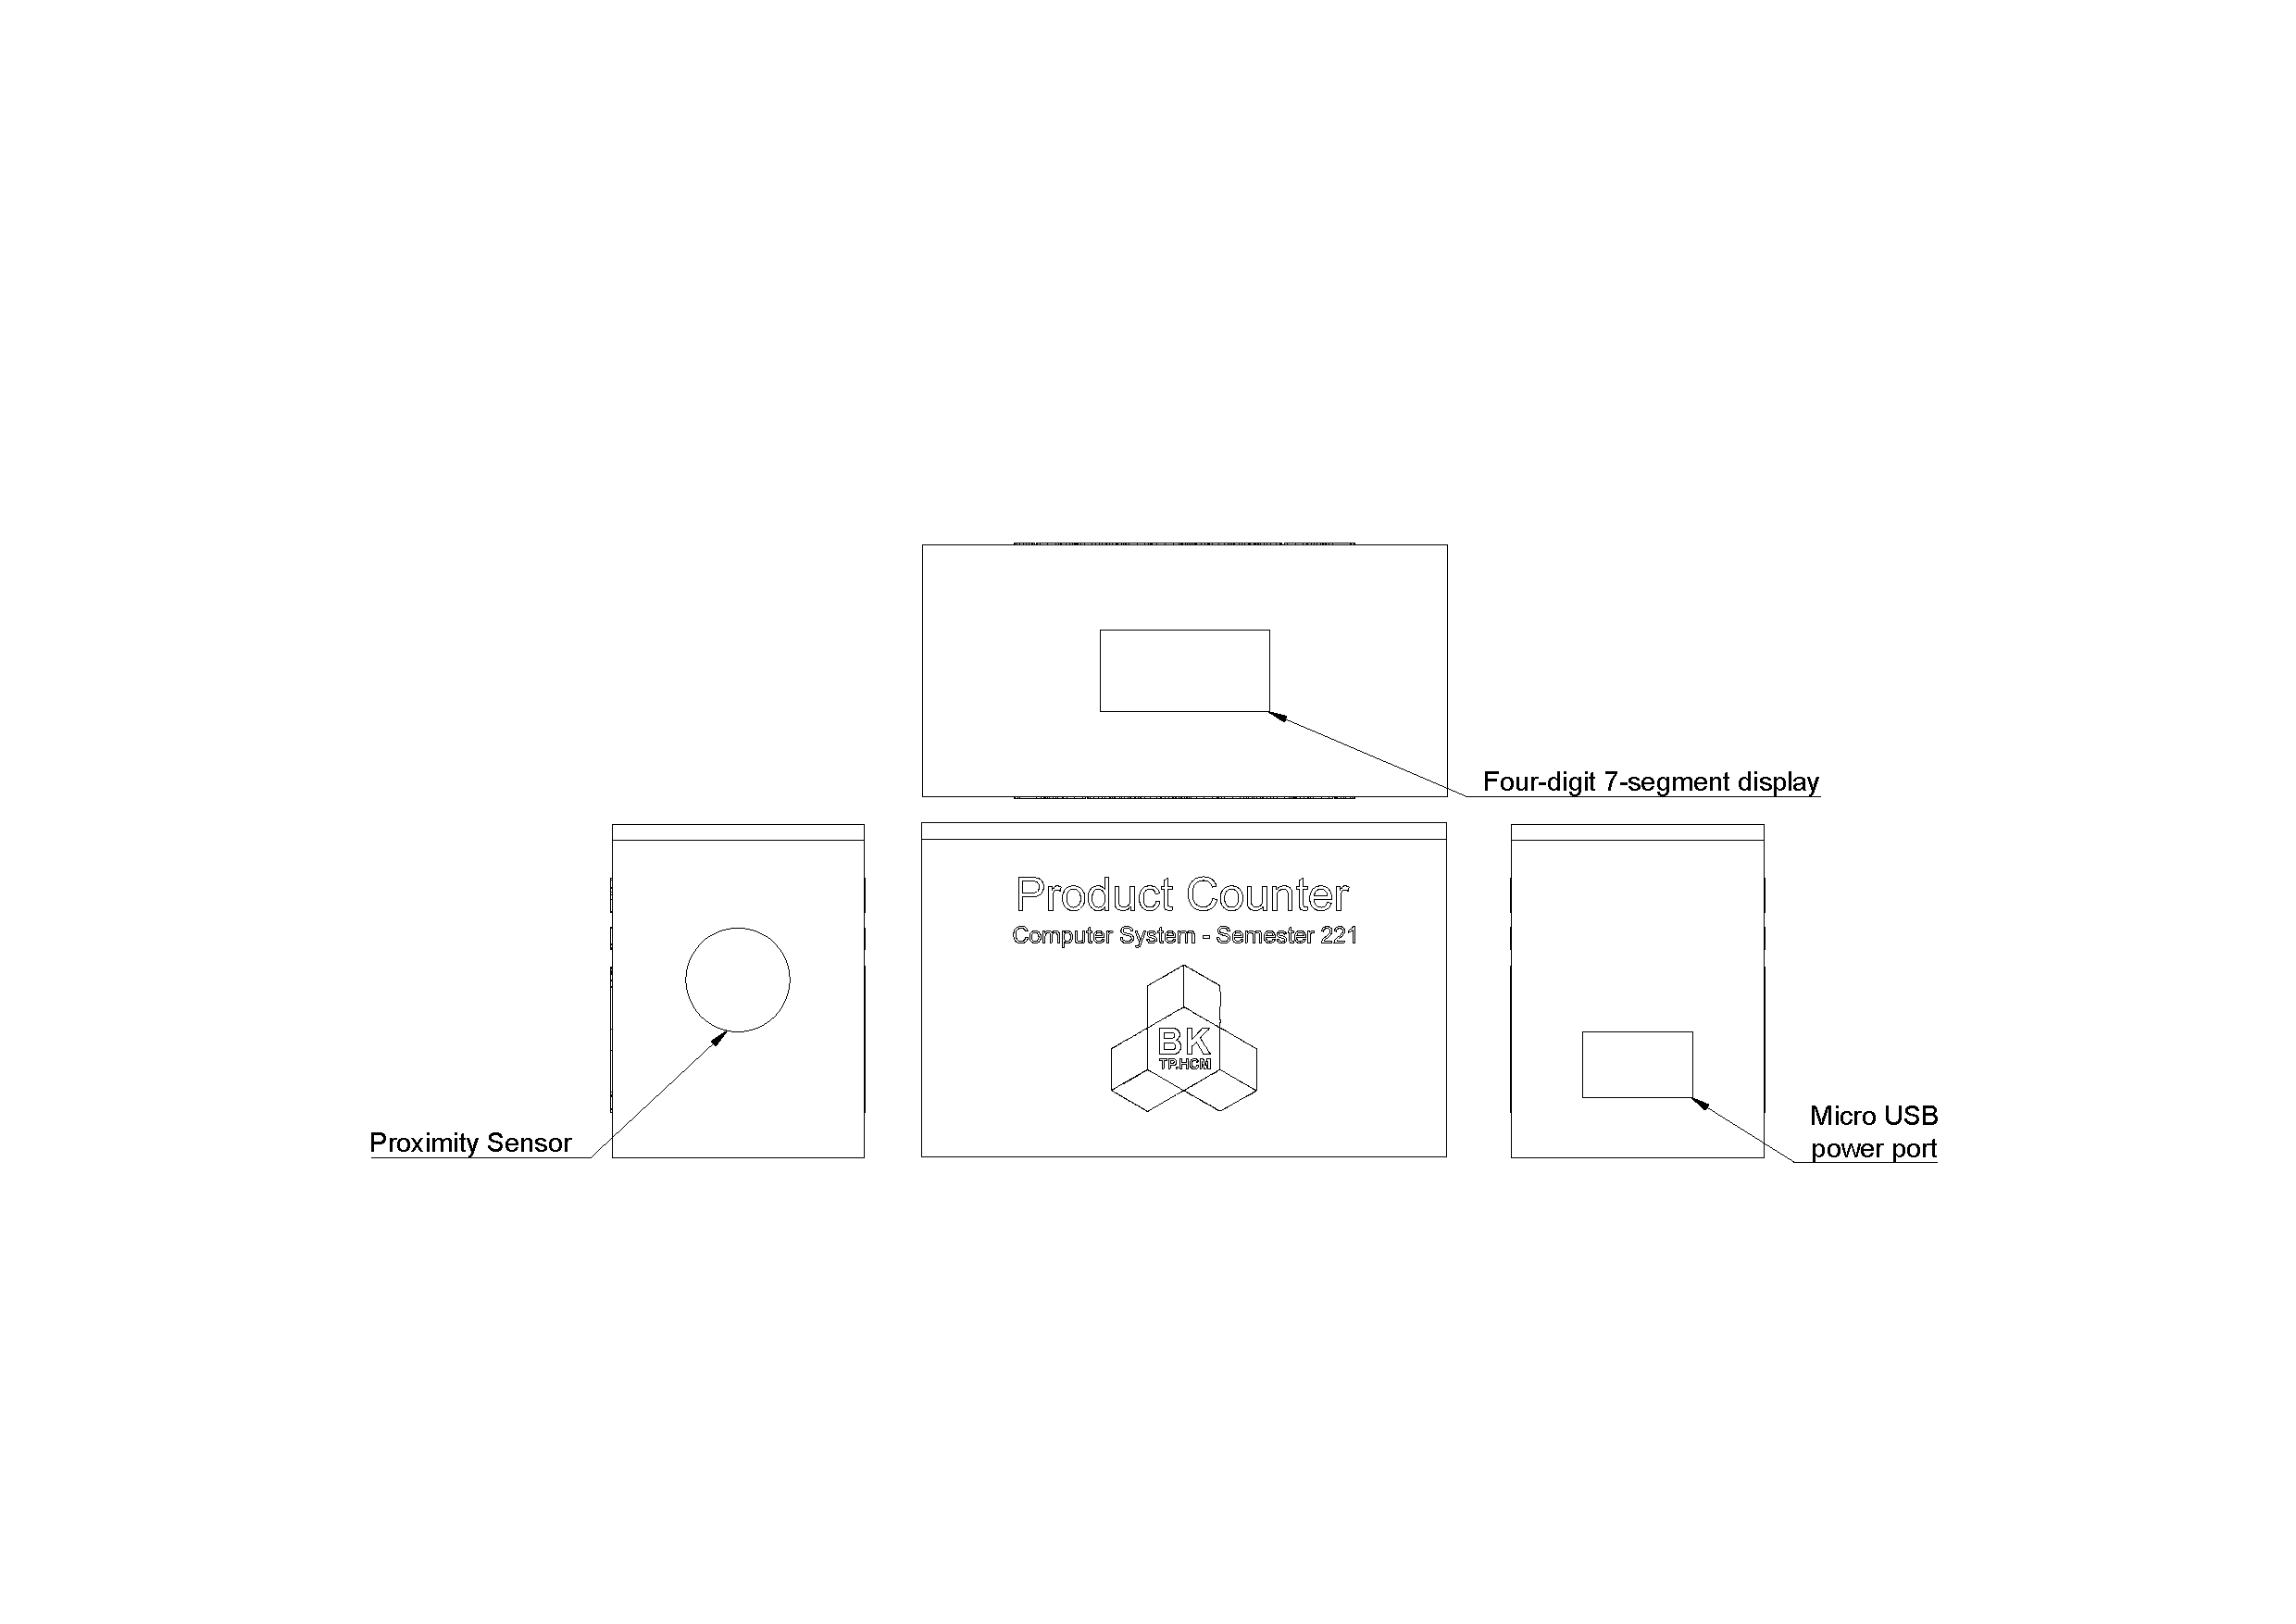
\includegraphics[scale=0.5]{images/model_schem_no_dim.pdf}
\caption{2D design of the case}
\end{figure}

\begin{figure}[H]
\centering
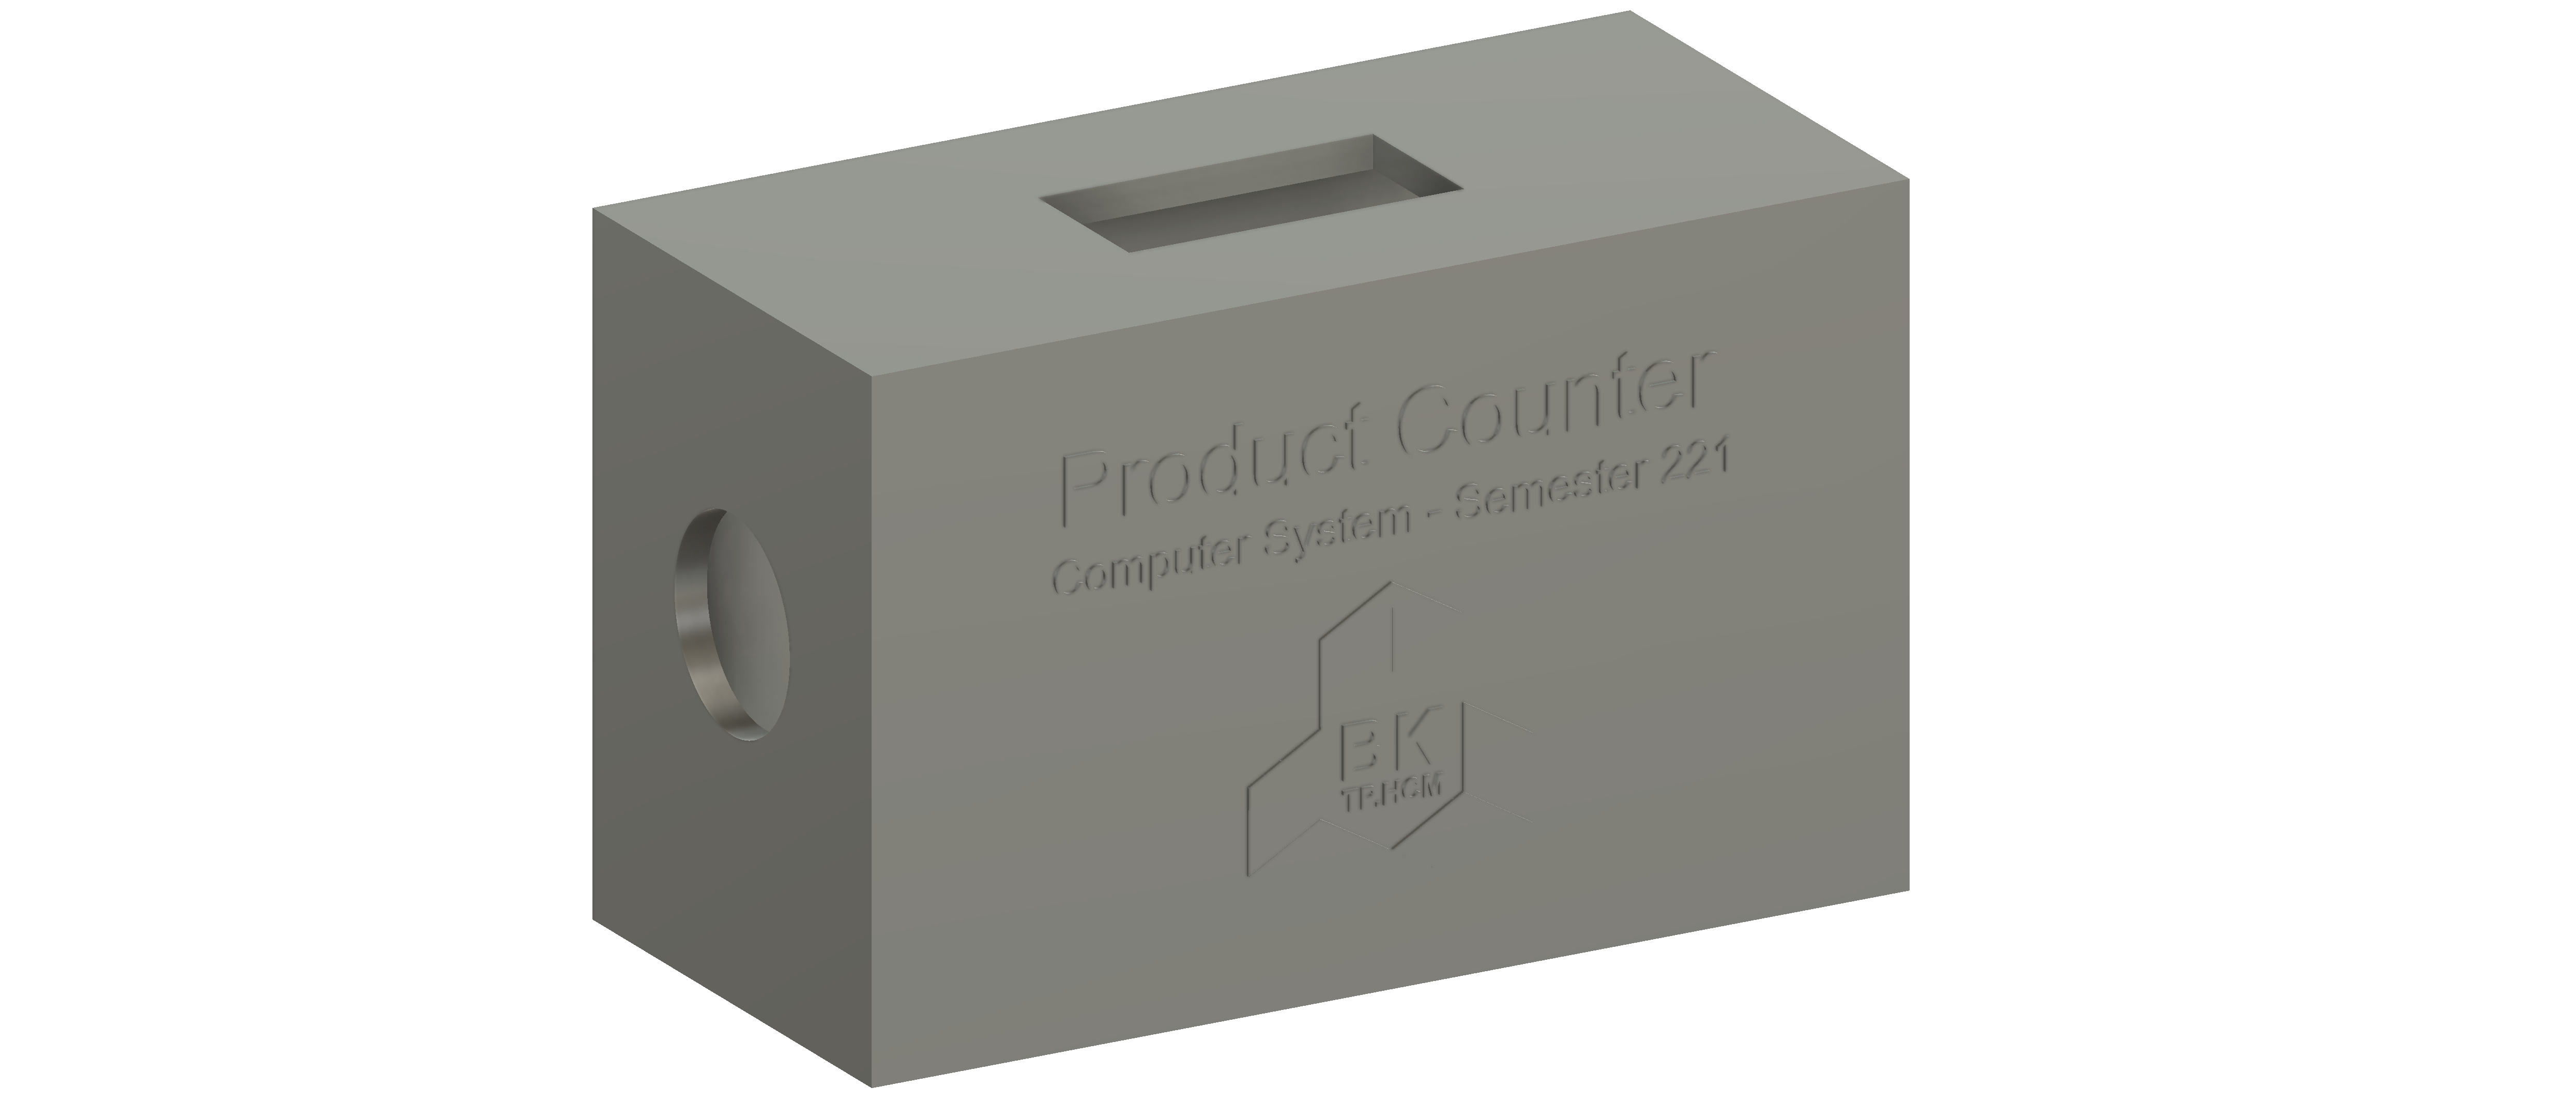
\includegraphics[scale=0.1]{images/device_3d.png}
\caption{3D design of the case}
\end{figure}
\chapter{Software}

\section{Keil-C and Pico Template}
We will use Keil-C compiler, along with µVision IDE. Since there is ARM Cortex M0+ support, but no direct support for Raspberry Pi Pico, we need to rely on a third-party template. GorgonMeducer's Pico\_Template \cite{pico_mdk}, which available free on GitHub, provide an ``out-of-the-box'' experience for newbie developers use Pico with Keil.

Assume you have installed packages for ARM Cortex M0+, to use GorgonMeducer's Pico\_Template, clone the repository with recursive mode to clone entire repo (including pico-sdk). Then install packages that end with \texttt{.pack} extension. 
\begin{minted}{bash}
git clone https://github.com/GorgonMeducer/Pico_Template --recursive
\end{minted}

The \texttt{main.c} file is the main program code that we will write our code on.
The µVision project is located in \texttt{./project/mdk} folder.

\section{Built-in functions}
\begin{itemize}
\item \mintinline{c}{void gpio_init(uint gpio)}: Initialize a GPIO pin.
\item \mintinline{c}{static void gpio_set_dir (uint gpio, bool out)}: Set a single GPIO direction, \texttt{out = GPIO\_OUT / GPIO\_IN}.
\item \mintinline{c}{static void gpio_put (uint gpio, bool value)}: Drive a single GPIO high/low.
\item \mintinline{c}{static bool gpio_get (uint gpio)}: Get state of a single specified GPIO.
\item \mintinline{c}{void sleep_ms(int milisecond)}: Pause and wait current thread for \texttt{milisecond} ms.
\end{itemize}

\section{Implement hardware with code}
\subsection{Read states of proximity sensor}
\begin{minted}{c}
gpio_get(IR);
\end{minted}

\subsection{Drive four-digit 7-segment display}
First, we define an array for characters from 0 to F and an array for storing data of LEDs.
\begin{minted}{c}
unsigned char LED_0F[] = {
// 0     1      2    3     4     5      6    7     8     9
  0xC0, 0xF9, 0xA4, 0xB0, 0x99, 0x92, 0x82, 0xF8, 0x80, 0x90, 
// A     b     C     d     E     F     -    off
  0x8C, 0xBF, 0xC6, 0xA1, 0x86, 0x8E, 0xbf, 0xFF
};

unsigned char LED[4] = {17,17,17,17};
\end{minted}

\texttt{LED\_OUT} function will send data bit by bit to \texttt{DIO} pin.

\begin{minted}{c}
void LED_OUT(unsigned char X) {
  unsigned char i;
  for (i = 8; i >= 1; i--) {
    if (X & 0x80) {
      gpio_put(DIO, 1);
    } else {
      gpio_put(DIO, 0);
    }
    X <<= 1;
    gpio_put(SCLK, 0);
    gpio_put(SCLK, 1);
  }
}
\end{minted}

Example: \texttt{X = 0xC0} (displaying 0 on the LED)
\begin{itemize}
\item \texttt{11000000 and 10000000 = 10000000} $\implies$ Output \texttt{1} to \texttt{DIO}
\item \texttt{10000000 and 10000000 = 10000000} $\implies$ Output \texttt{1} to \texttt{DIO}
\item \texttt{00000000 and 10000000 = 00000000} $\implies$ Output \texttt{0} to \texttt{DIO}
\item \texttt{00000000 and 10000000 = 00000000} $\implies$ Output \texttt{0} to \texttt{DIO}
\item ...
\end{itemize}
As a result, \led{0} is displayed on the LED.

The above function output only one character. We need to write a function to output all four digits on the LED. The function takes data of \texttt{LED[]} array and output to the 7-segment LEDs. The number to be displayed on the screen will be specified as the corresponding hexadecimal form in \texttt{LED\_0F} and inserted into the 7-segment display as the binary converted from hexadecimal in \texttt{LED\_0F}.

\begin{minted}{c}
void LED4_Display(void) {
  unsigned char * led_table;
  unsigned char i;

  led_table = LED_0F + LED[0];
  i = * led_table;
  LED_OUT(i);
  LED_OUT(0x08); // 1000
  gpio_put(RCLK, 0);
  gpio_put(RCLK, 1);

  led_table = LED_0F + LED[1];
  i = * led_table;
  LED_OUT(i);
  LED_OUT(0x04); // 0100
  gpio_put(RCLK, 0);
  gpio_put(RCLK, 1);

  led_table = LED_0F + LED[2];
  i = * led_table;
  LED_OUT(i);
  LED_OUT(0x02); //0010
  gpio_put(RCLK, 0);
  gpio_put(RCLK, 1);

  led_table = LED_0F + LED[3];
  i = * led_table;
  LED_OUT(i);
  LED_OUT(0x01); //0001
  gpio_put(RCLK, 0);
  gpio_put(RCLK, 1);
}
\end{minted}

Before displaying we need to determine the hexadecimal data to be displayed. \texttt{led\_table = LED\_0F + LED[0]} will point to the hexadecimal data that needed to output to the LED. The procedure is similar to other LEDs.

\subsection{Separate integer into digits}
\begin{minted}{c}
void Num2LED(int num) {
  LED[3] = num % 10;
  LED[2] = (num /= 10) % 10;
  LED[1] = (num /= 10) % 10;
  LED[0] = num / 10;
  LED4_Display();
}
\end{minted}
Example: 1234
\begin{itemize}
\item \mintinline{c}{LED[3] = num % 10 = 1234 % 10 = 4}
\item \mintinline{c}{LED[2] = (num /= 10) % 10 = 123 % 10 = 3}
\item \mintinline{c}{LED[1] = (num /= 10) % 10 = 12 % 10 = 2}
\item \mintinline{c}{LED[0] = num / 10 = 12 / 10 = 1}
\end{itemize}

\subsection{Using the buzzer}
The buzzer will ``beep'' for a short period of time, so we will set the buzzer on for 100ms then off.
\begin{minted}{c}
gpio_put(BUZZER, 1);
sleep_ms(100);
gpio_put(BUZZER, 0);
\end{minted}


\chapter{Implementation result}
\section{Result}
\begin{figure}[H]
\centering
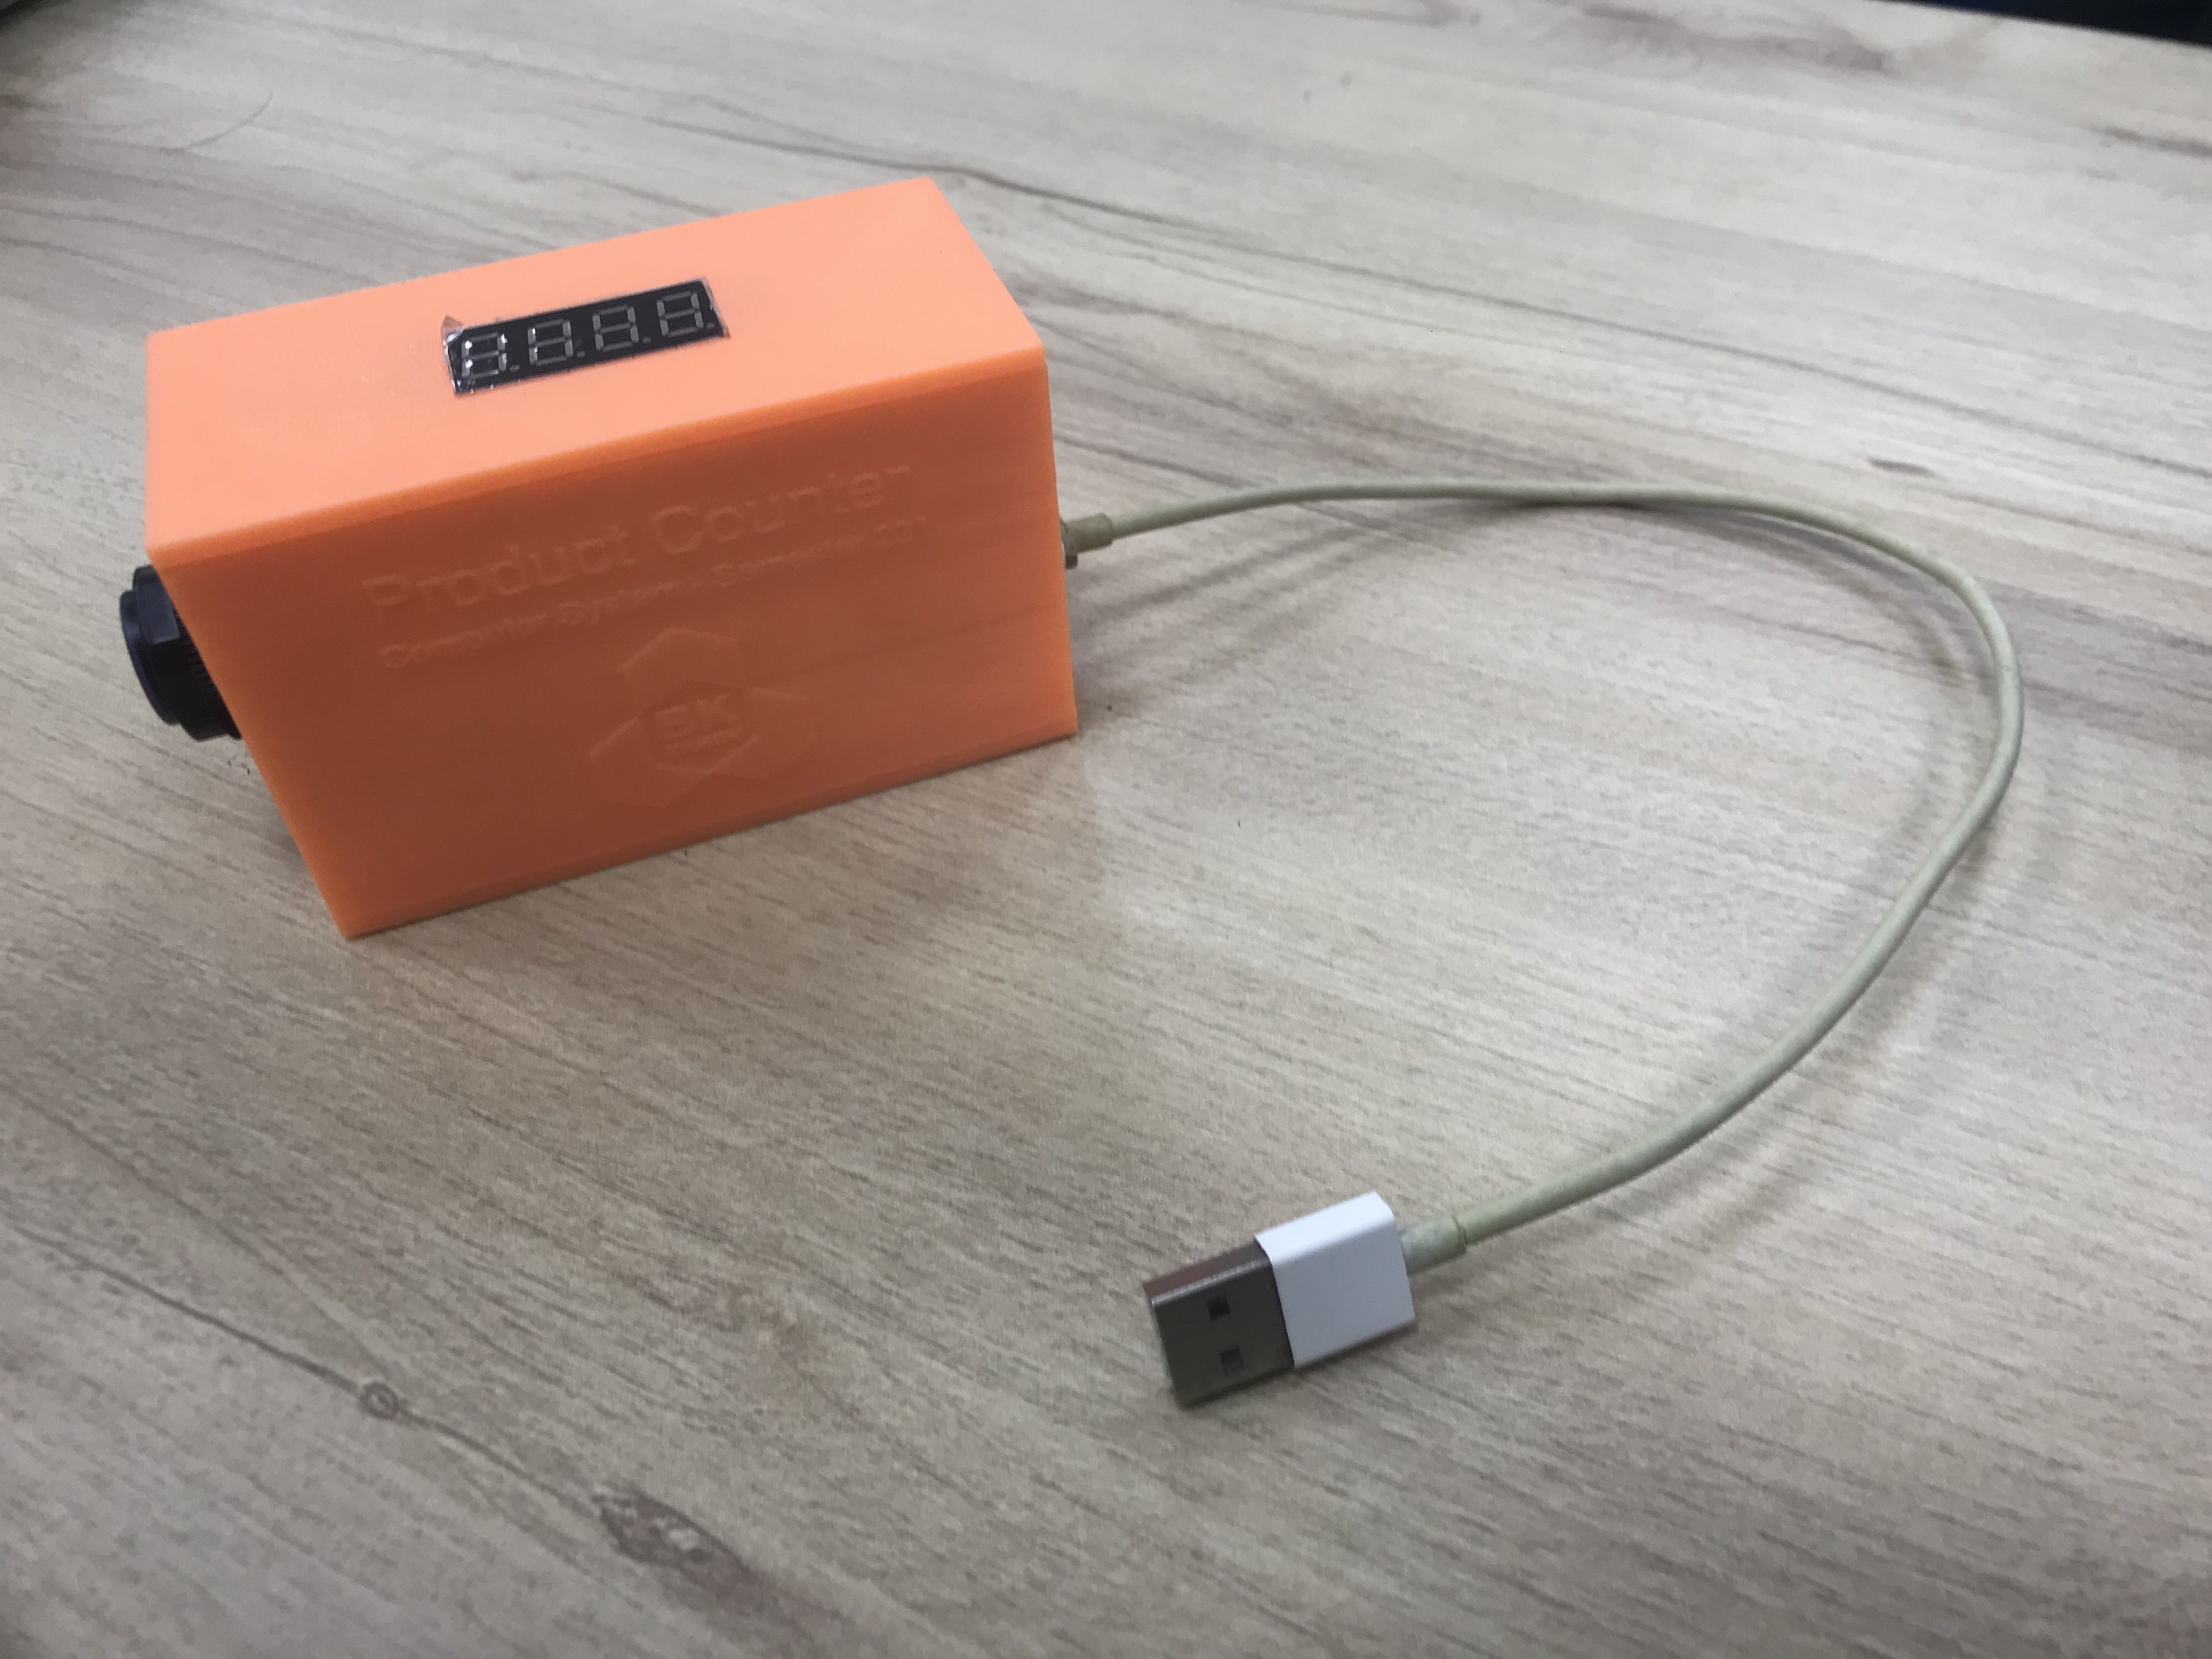
\includegraphics[scale=0.07]{images/device.jpg}
\caption{The complete device}
\end{figure}

\begin{figure}[H]
\centering
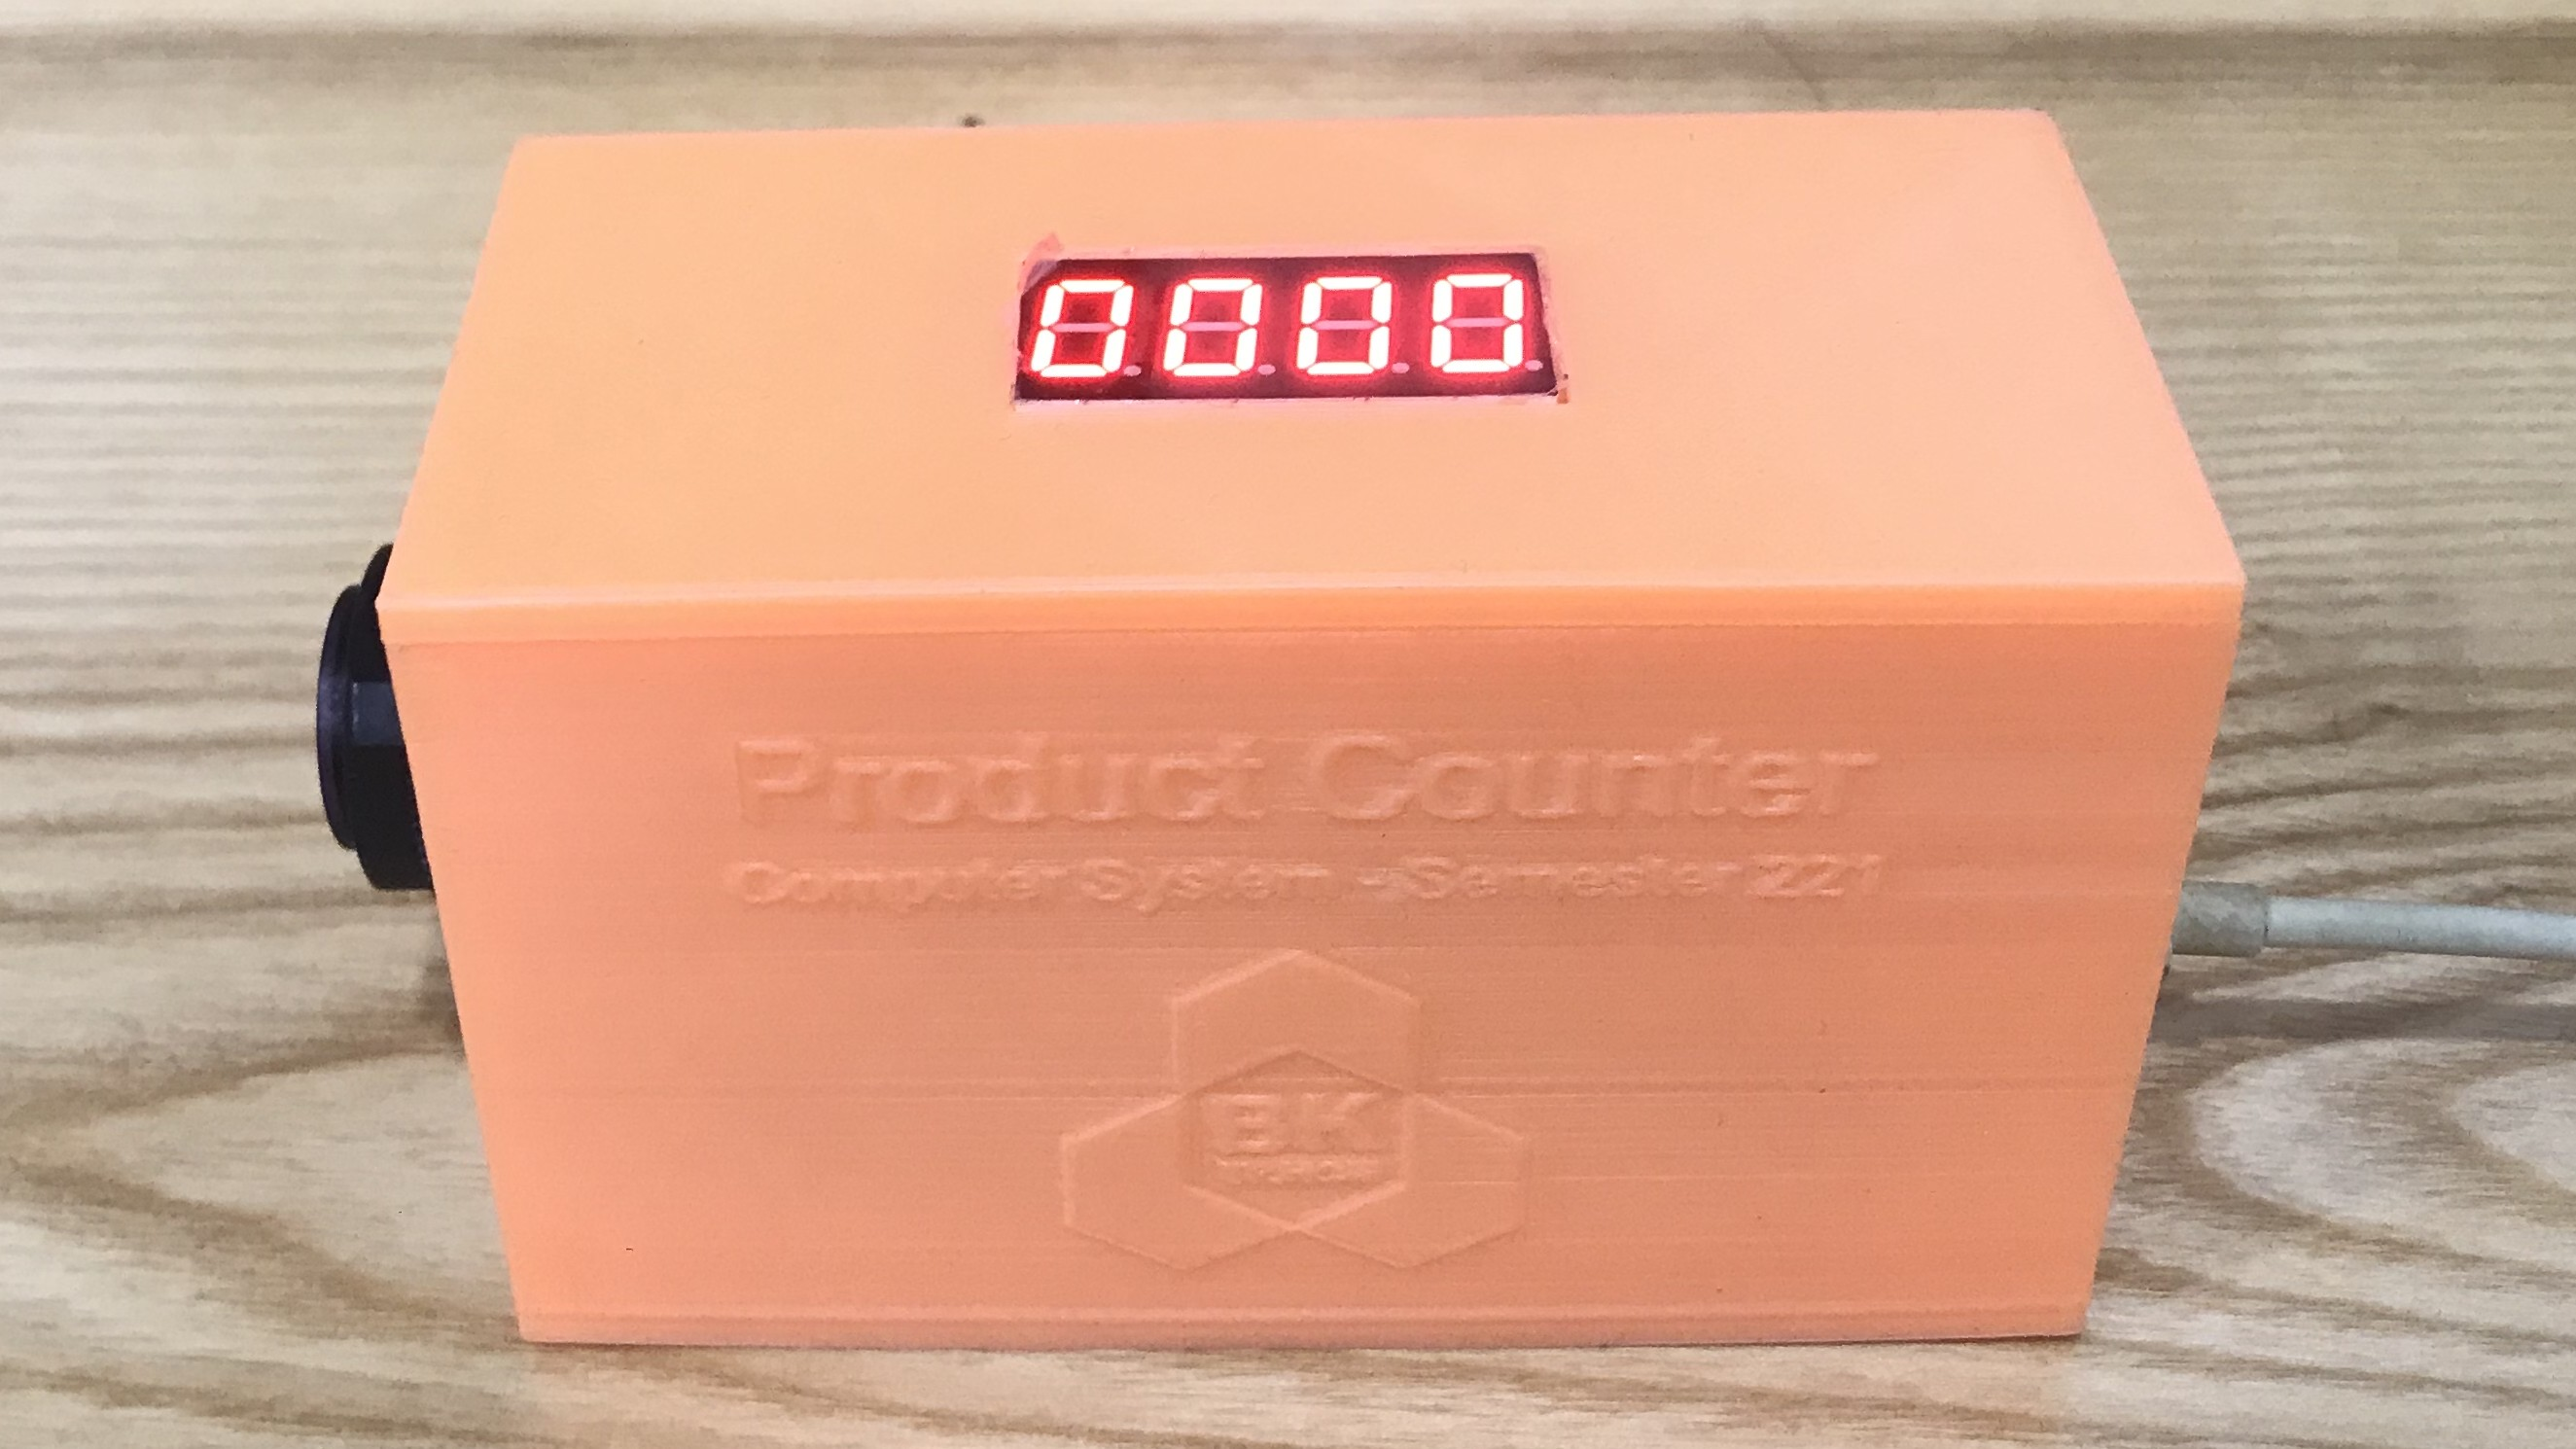
\includegraphics[scale=0.07]{images/counter_0.jpg}
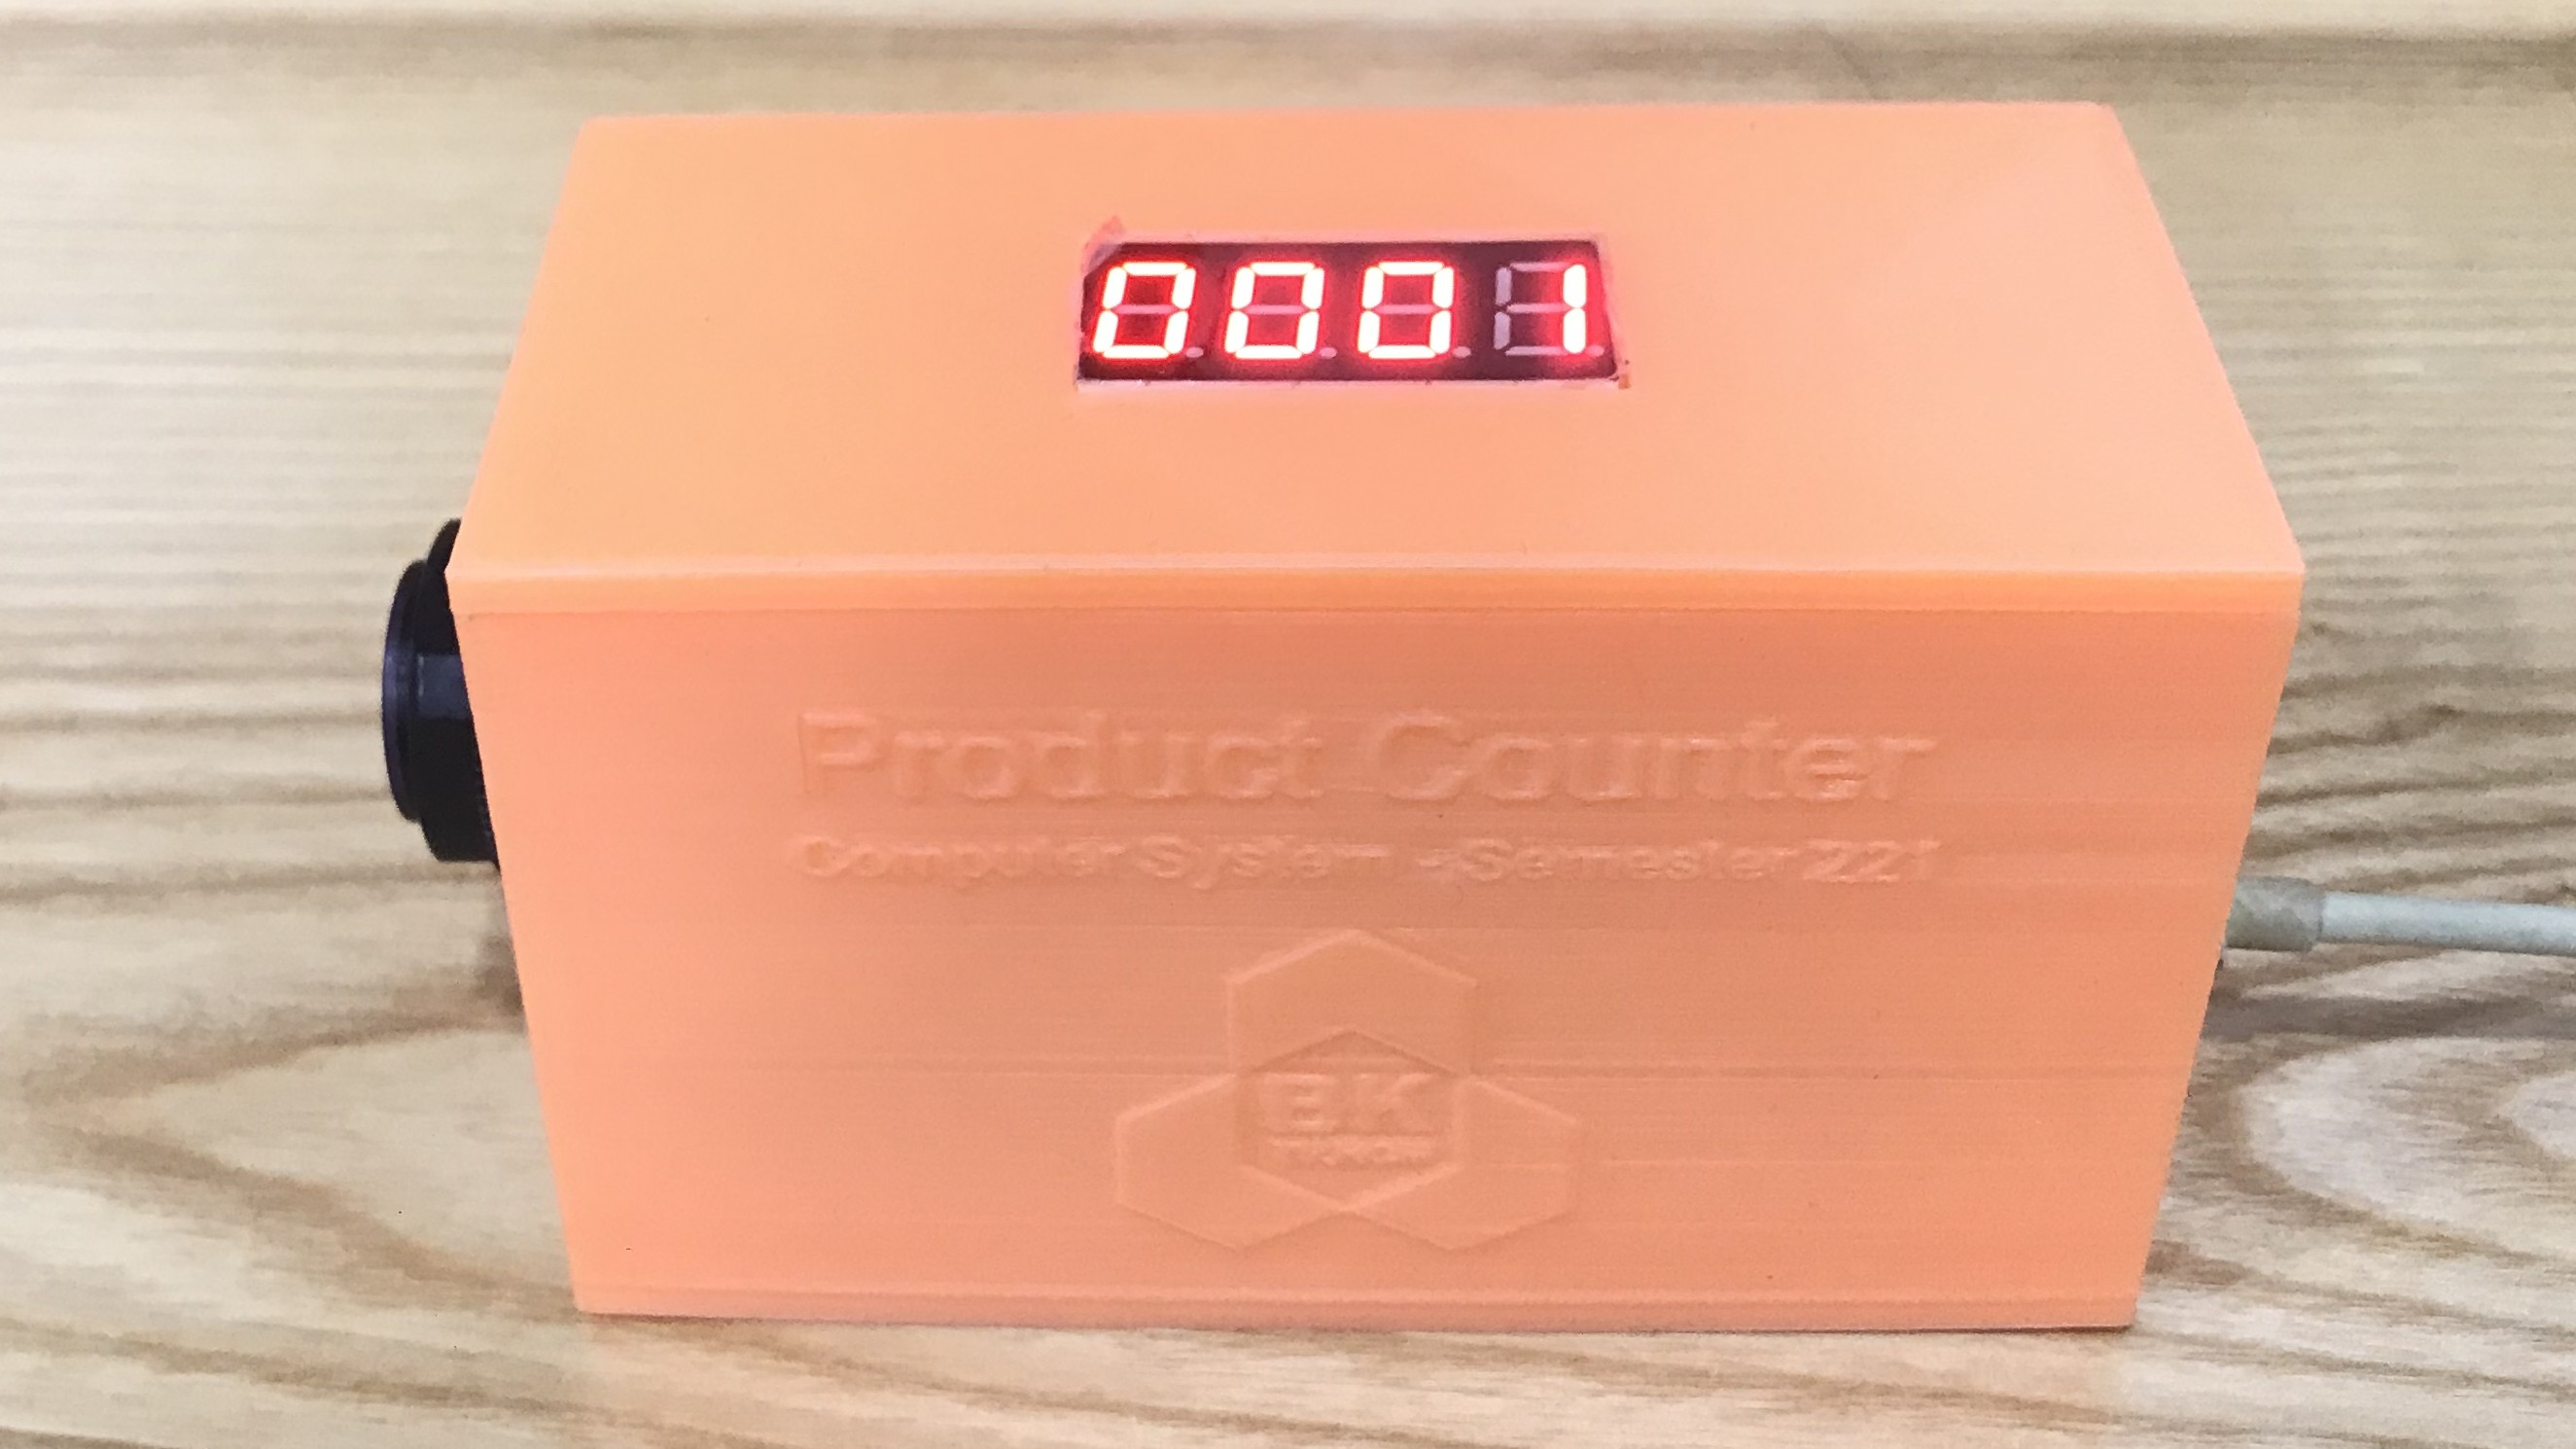
\includegraphics[scale=0.07]{images/counter_1.jpg}
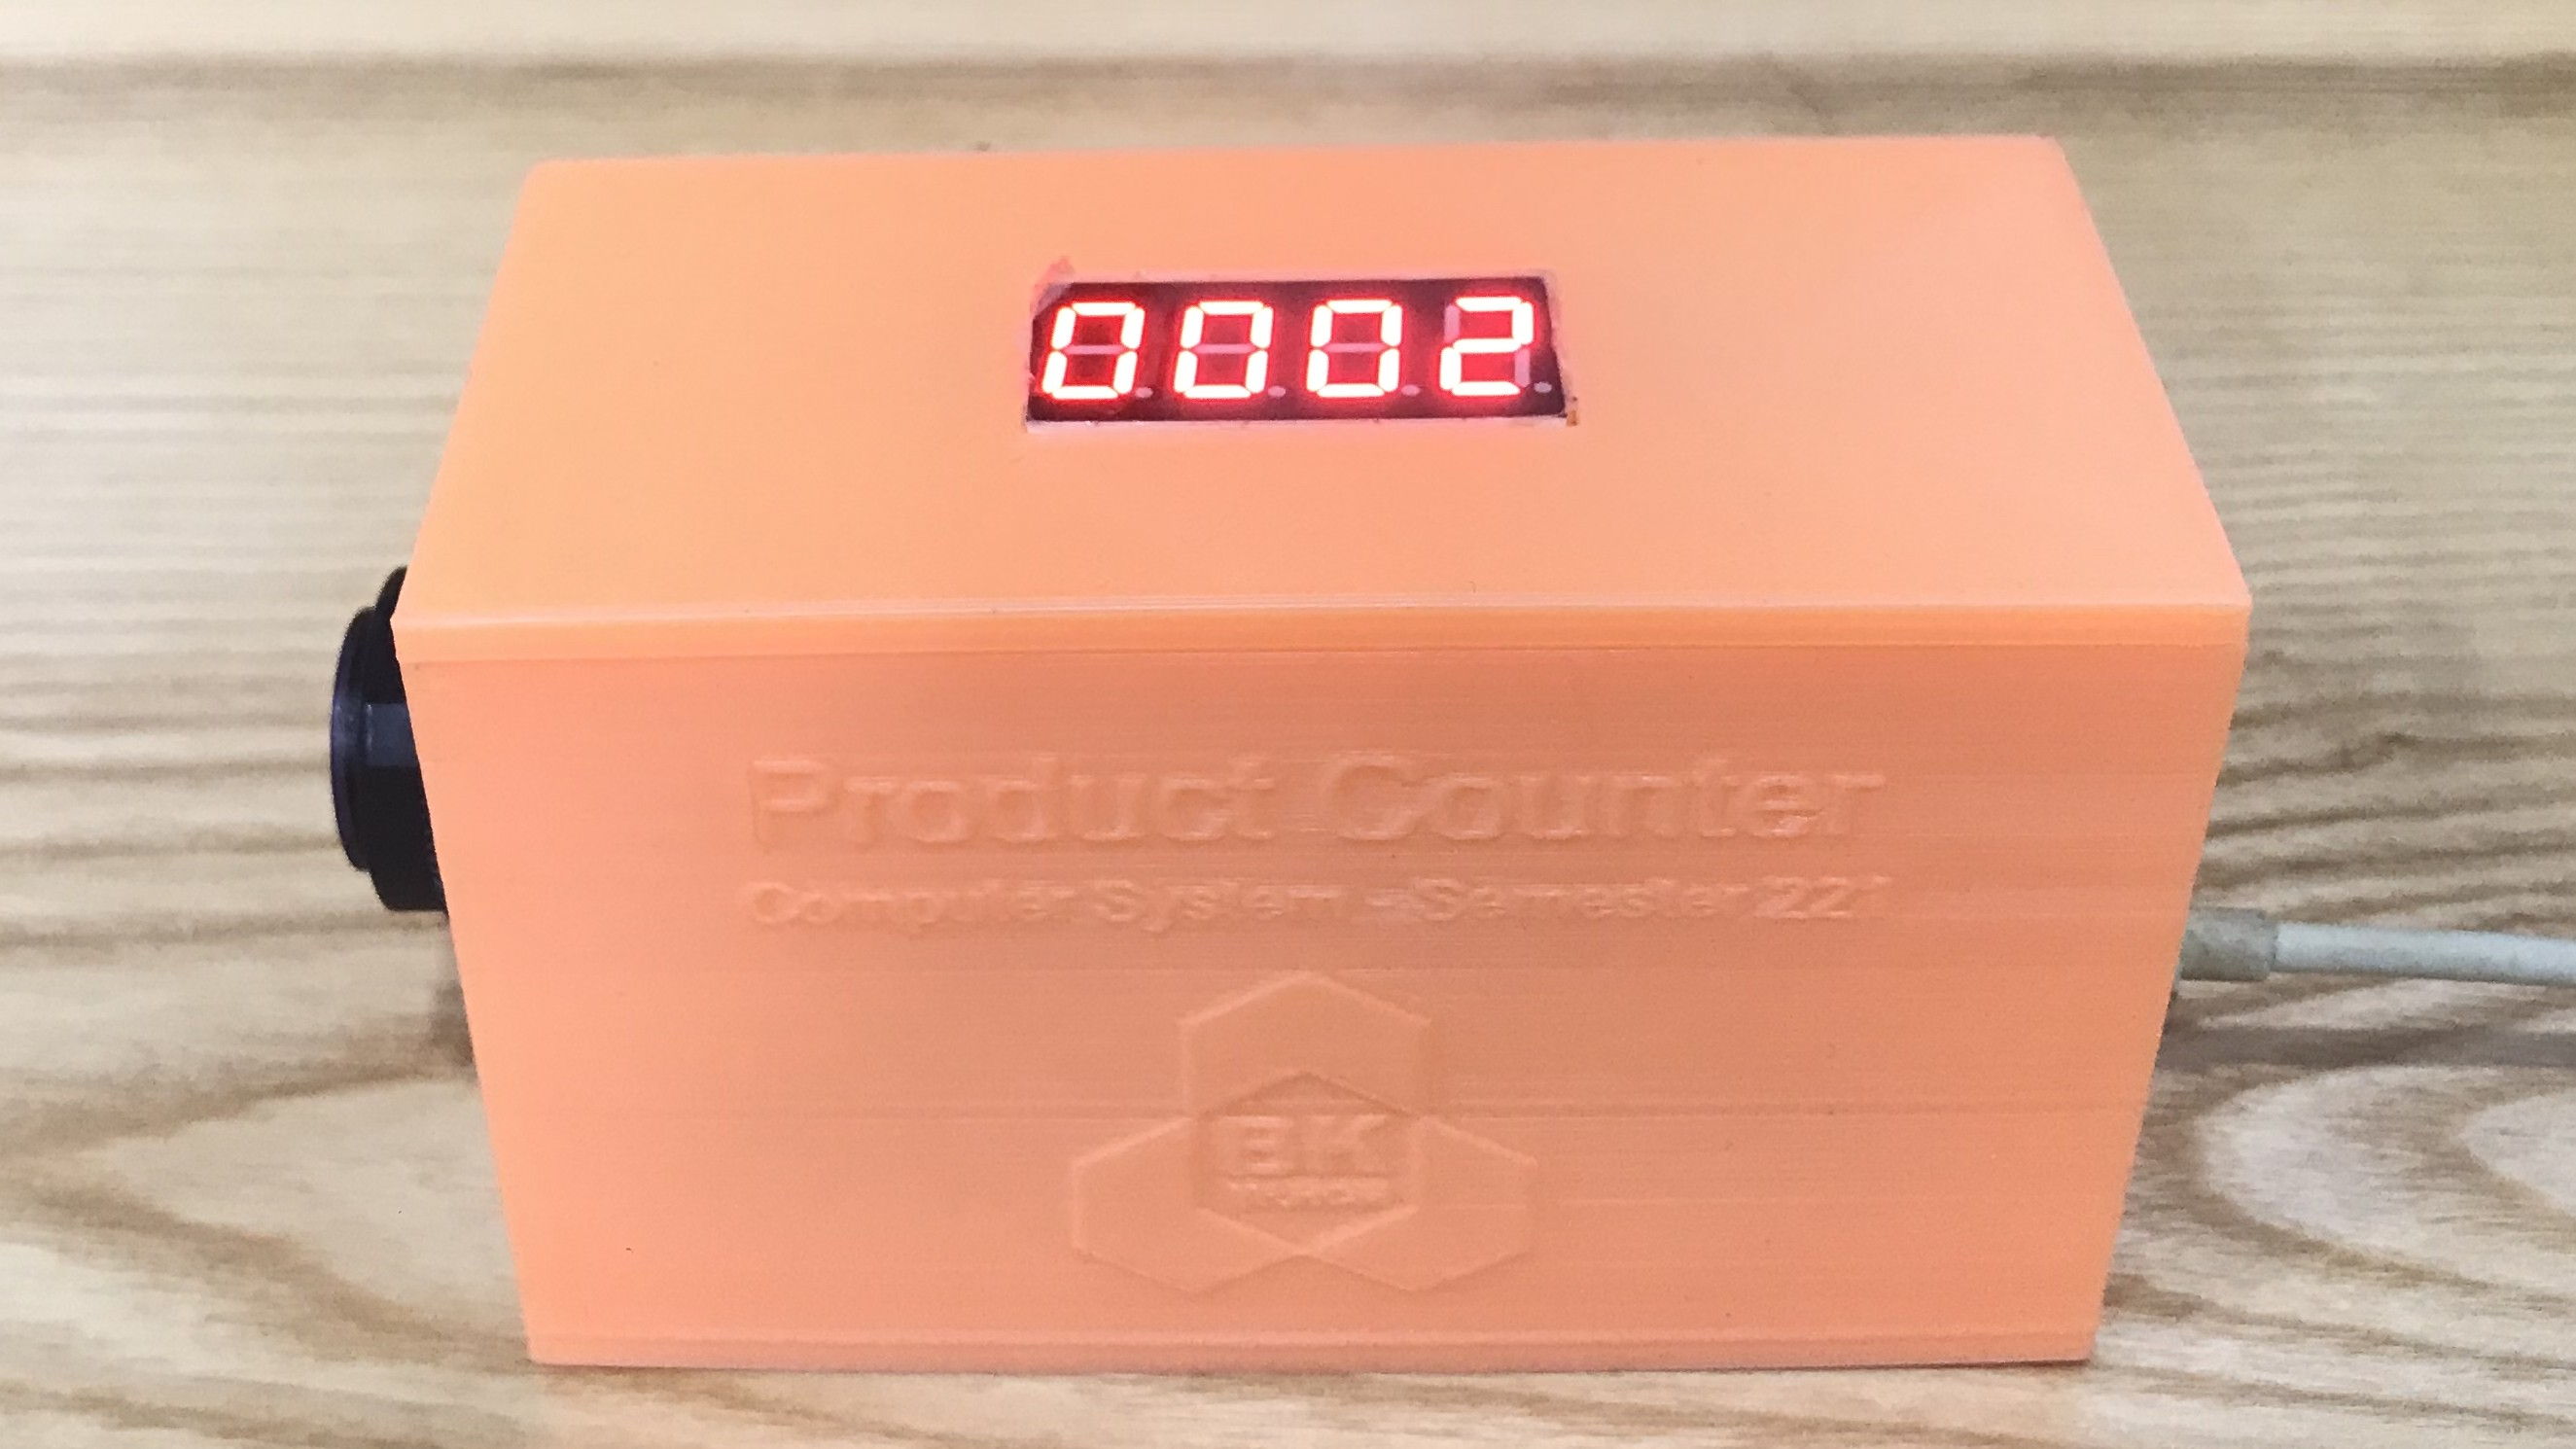
\includegraphics[scale=0.07]{images/counter_2.jpg}\\
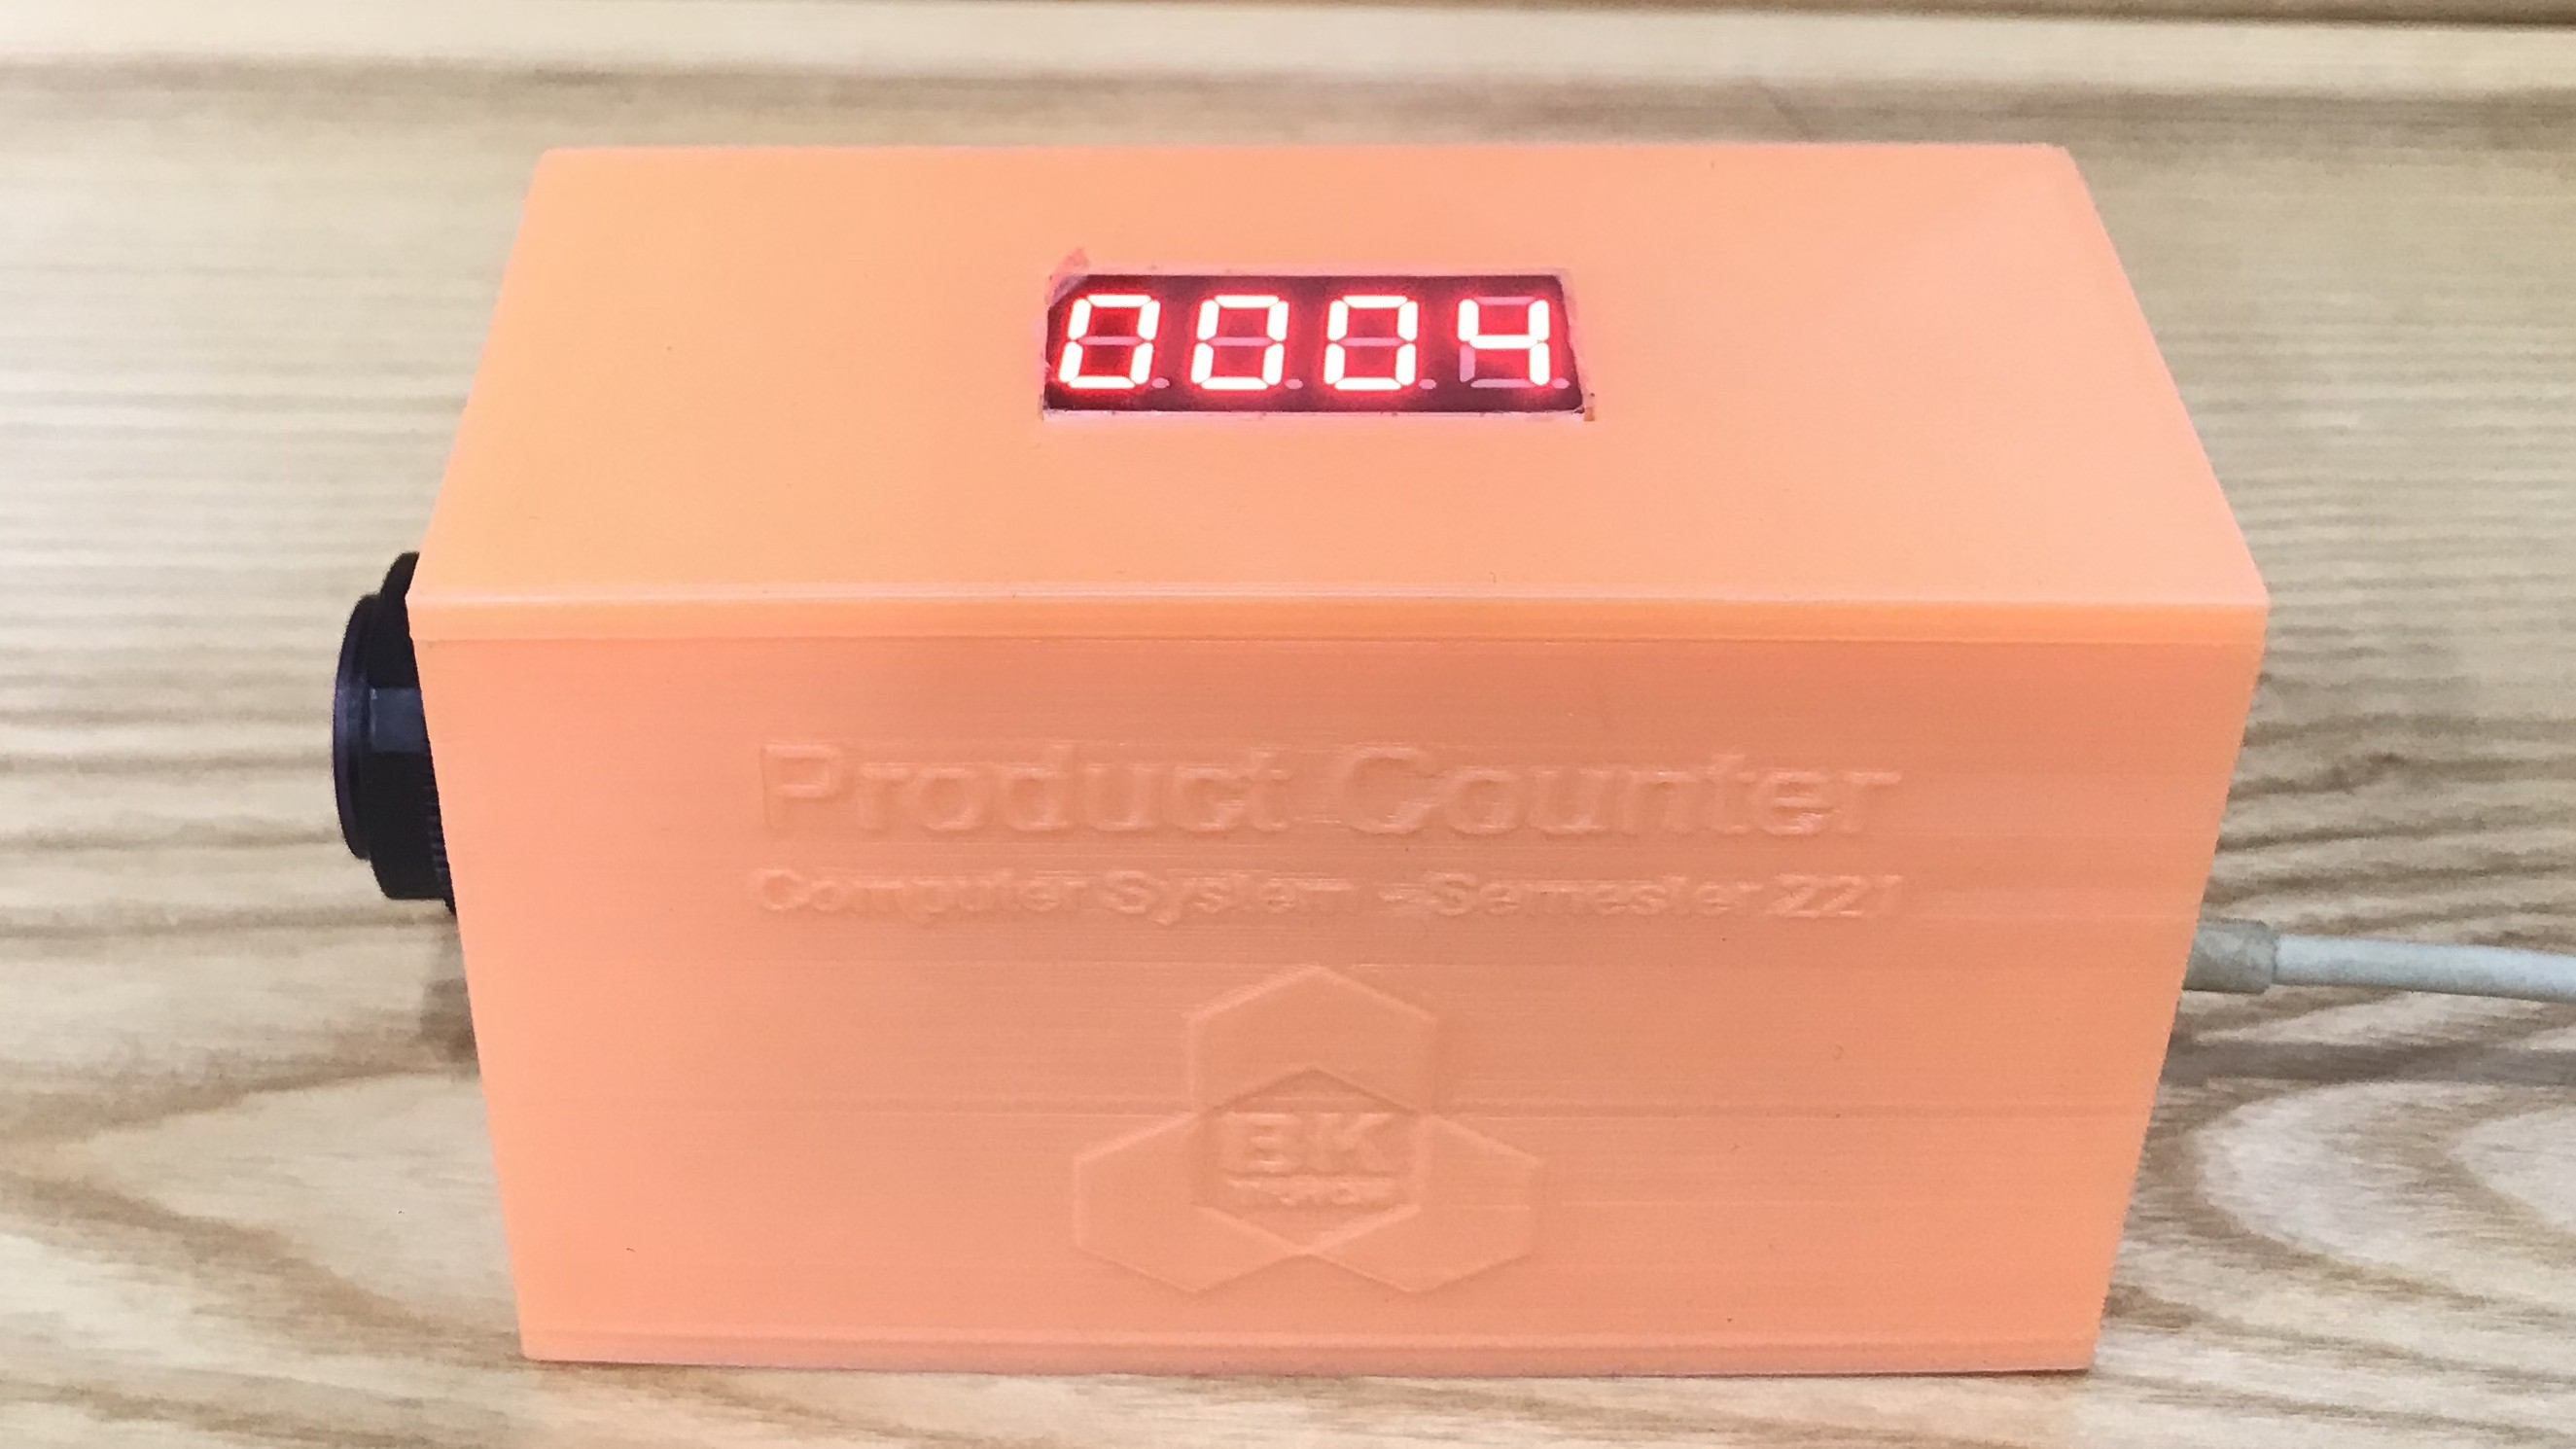
\includegraphics[scale=0.07]{images/counter_4.jpg}
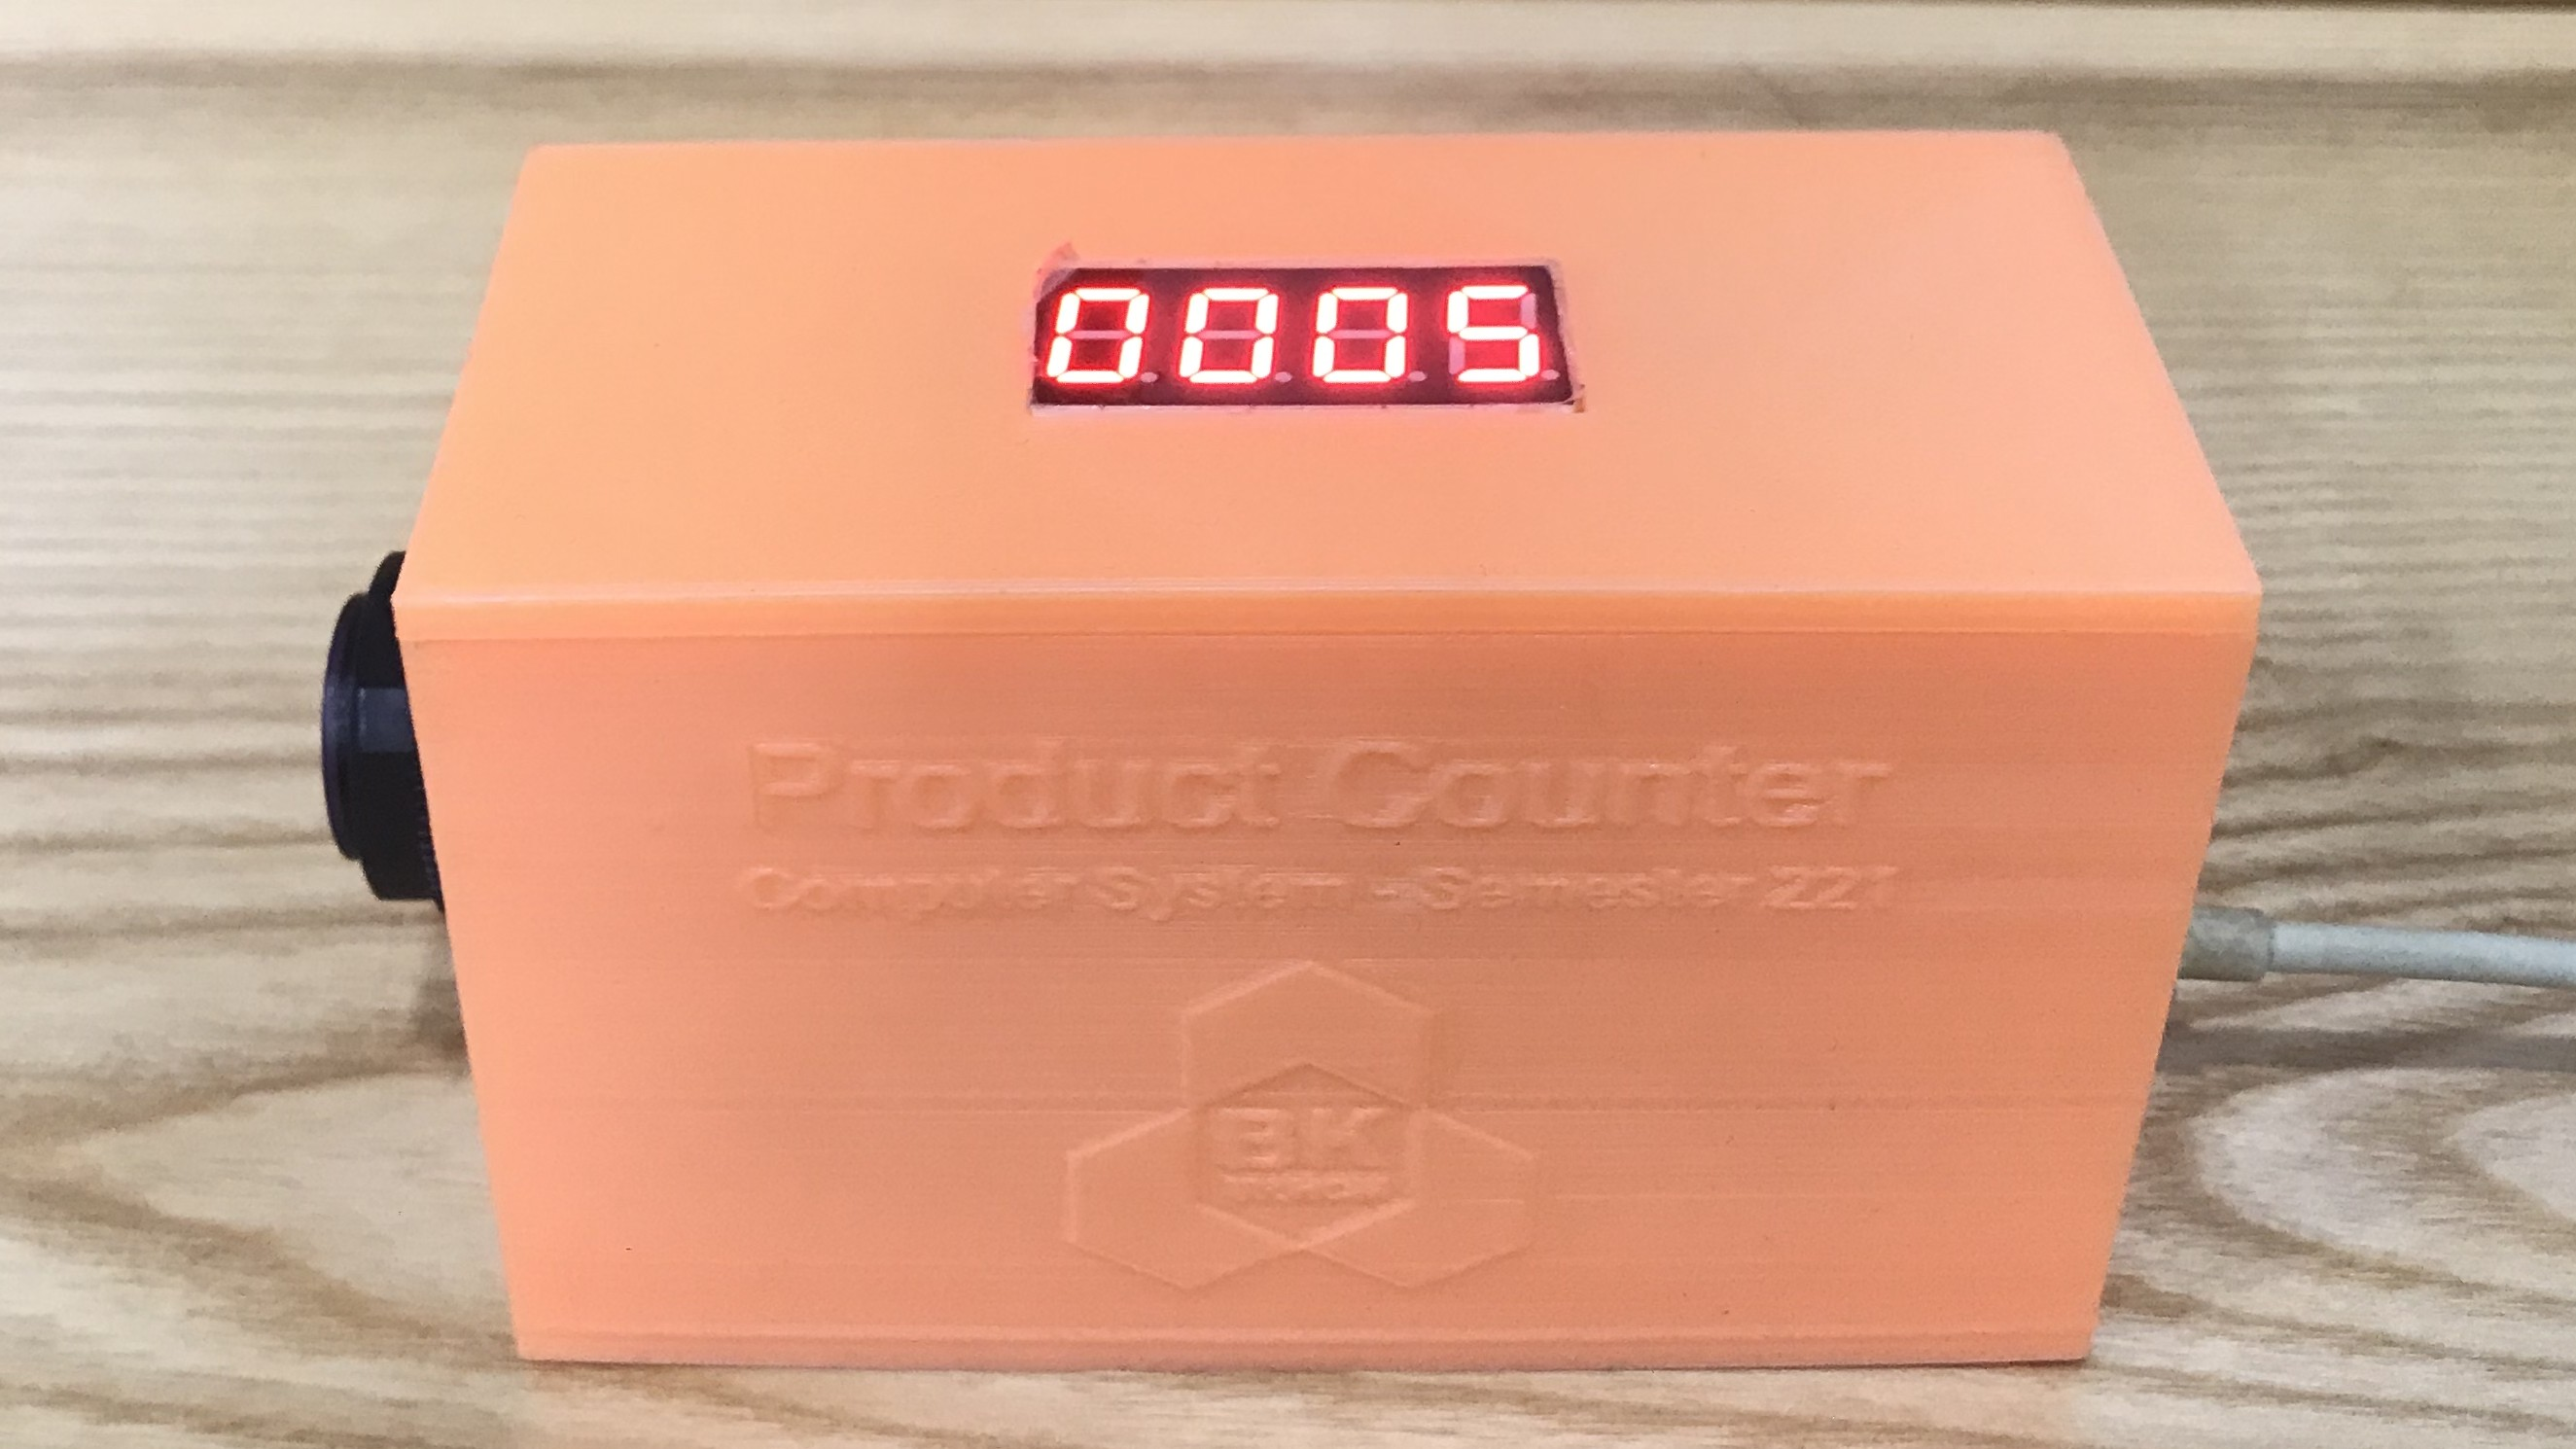
\includegraphics[scale=0.07]{images/counter_5.jpg}
\caption{The device counts and ``beep'' when an object passed by}
\end{figure}

\section{Source code}
\begin{minted}{c}
// SOME CODES ARE PREDEFINED AND INITIALIZED. DO NOT EDIT.
/*========================= INCLUDES ===================================*/
#include "pico/stdlib.h"
#include "perf_counter.h"

#if defined(__PICO_USE_LCD_1IN3__) && __PICO_USE_LCD_1IN3__
#include "DEV_Config.h"
#include "LCD_1In3.h"
#include "GLCD_Config.h"
#endif

#include <stdio.h>
#include "RTE_Components.h"

#if defined(RTE_Compiler_EventRecorder) && defined(USE_EVR_FOR_STDOUR)
  #include <EventRecorder.h>
#endif

/*========================= MACROS =====================================*/
#define TOP	(0x1FFF)

/*========================= MACROFIED FUNCTIONS ========================*/
#define ABS(__N)((__N) < 0 ? -(__N) : (__N))
#define _BV(__N)((uint32_t) 1 << (__N))

/*============================== CONSTANTS =============================*/
#define IR 16
#define BUZZER 17
#define DIO 18
#define RCLK 19
#define SCLK 20

/*========================= TYPES ======================================*/
/*========================= GLOBAL VARIABLES ===========================*/
unsigned char LED_0F[] = {
// 0     1      2    3     4     5      6    7     8     9
  0xC0, 0xF9, 0xA4, 0xB0, 0x99, 0x92, 0x82, 0xF8, 0x80, 0x90, 
// A     b     C     d     E     F     -    off
  0x8C, 0xBF, 0xC6, 0xA1, 0x86, 0x8E, 0xbf, 0xFF
};

unsigned char LED[4] = {};
/*========================= LOCAL VARIABLES ============================*/
/*========================= PROTOTYPES =================================*/
/*========================= IMPLEMENTATION =============================*/
void SysTick_Handler(void) {}

static void system_init(void) {
  extern void SystemCoreClockUpdate();

  SystemCoreClockUpdate();
  /*! \note if you do want to use SysTick in your application, please use 
   *!       init_cycle_counter(true); 
   *!       instead of 
   *!       init_cycle_counter(false); 
   */
  init_cycle_counter(false);

  #if defined(RTE_Compiler_EventRecorder) && defined(USE_EVR_FOR_STDOUR)
  EventRecorderInitialize(0, 1);
  #endif

  gpio_init(DIO);
  gpio_set_dir(DIO, GPIO_OUT);

  gpio_init(SCLK);
  gpio_set_dir(SCLK, GPIO_OUT);

  gpio_init(RCLK);
  gpio_set_dir(RCLK, GPIO_OUT);

  gpio_init(BUZZER);
  gpio_set_dir(BUZZER, GPIO_OUT);

  gpio_init(IR);
  gpio_set_dir(IR, GPIO_IN);

  #if defined(__PICO_USE_LCD_1IN3__) && __PICO_USE_LCD_1IN3__
  DEV_Delay_ms(100);

  if (DEV_Module_Init() != 0) {
    //assert(0);
  }

  DEV_SET_PWM(50);
  /* LCD Init */

  LCD_1IN3_Init(HORIZONTAL);
  LCD_1IN3_Clear(GLCD_COLOR_BLUE);

  for (int n = 0; n < KEY_NUM; n++) {
    dev_key_init(n);
  }
  #endif
}

void LED_OUT(unsigned char X) {
  unsigned char i;
  for (i = 8; i >= 1; i--) {
    if (X & 0x80) {
      gpio_put(DIO, 1);
    } else {
      gpio_put(DIO, 0);
    }
    X <<= 1;
    gpio_put(SCLK, 0);
    gpio_put(SCLK, 1);
  }
}

void LED4_Display(void) {
  unsigned char * led_table;
  unsigned char i;

  led_table = LED_0F + LED[0];
  i = * led_table;
  LED_OUT(i);
  LED_OUT(0x08); // 1000
  gpio_put(RCLK, 0);
  gpio_put(RCLK, 1); // store in shift register

  led_table = LED_0F + LED[1];
  i = * led_table;
  LED_OUT(i);
  LED_OUT(0x04); // 0100
  gpio_put(RCLK, 0);
  gpio_put(RCLK, 1);

  led_table = LED_0F + LED[2];
  i = * led_table;
  LED_OUT(i);
  LED_OUT(0x02); //0010
  gpio_put(RCLK, 0);
  gpio_put(RCLK, 1);

  led_table = LED_0F + LED[3];
  i = * led_table;
  LED_OUT(i);
  LED_OUT(0x01); //0001
  gpio_put(RCLK, 0);
  gpio_put(RCLK, 1);
}

void Num2LED(int num) {
  LED[3] = num % 10;
  LED[2] = (num /= 10) % 10;
  LED[1] = (num /= 10) % 10;
  LED[0] = num / 10;
  LED4_Display();
}

int main(void) {
  system_init();
  gpio_put(BUZZER, 0);
  sleep_ms(100);
  int count = 0;

  while (true) {
    Num2LED(count);
    if (gpio_get(IR) == 0) {
      count++;
      gpio_put(BUZZER, 1);
      sleep_ms(100);
      gpio_put(BUZZER, 0);

      while (gpio_get(IR) == 0)
        Num2LED(count);
    }
  }

  return 0;
}
\end{minted}

\chapter{Conclusion}
We have successfully created the product counter by using Raspberry Pi Pico. We also discover the working principle of the infrared proximity sensor, four-digit 7-segment display, and the buzzer. Furthermore, we have designed the 3D model case by using Autodesk Fusion 360. But the power supply devices still depend on the external source (5V phone charger, power bank, computer,...). In the future, we will integrate the battery into the device, create a button to reset the counter, optimize the size of the 3D printed case, and increase the accuracy of the sensor. 

\chapter{References}
\AtNextBibliography{\large}
\setlength\bibitemsep{5pt}
\nocite{*}
\printbibliography[heading=none]

\chapter{Appendix}
A larger version of wiring schematic and CAD design of 3D Printed case (1:1 scale) are listed below.

All program source codes and reports' \LaTeX \ source codes can be accessed at our GitHub repository: \url{https://github.com/superzeldalink/ProductCounter-Pico}.

\begin{landscape}
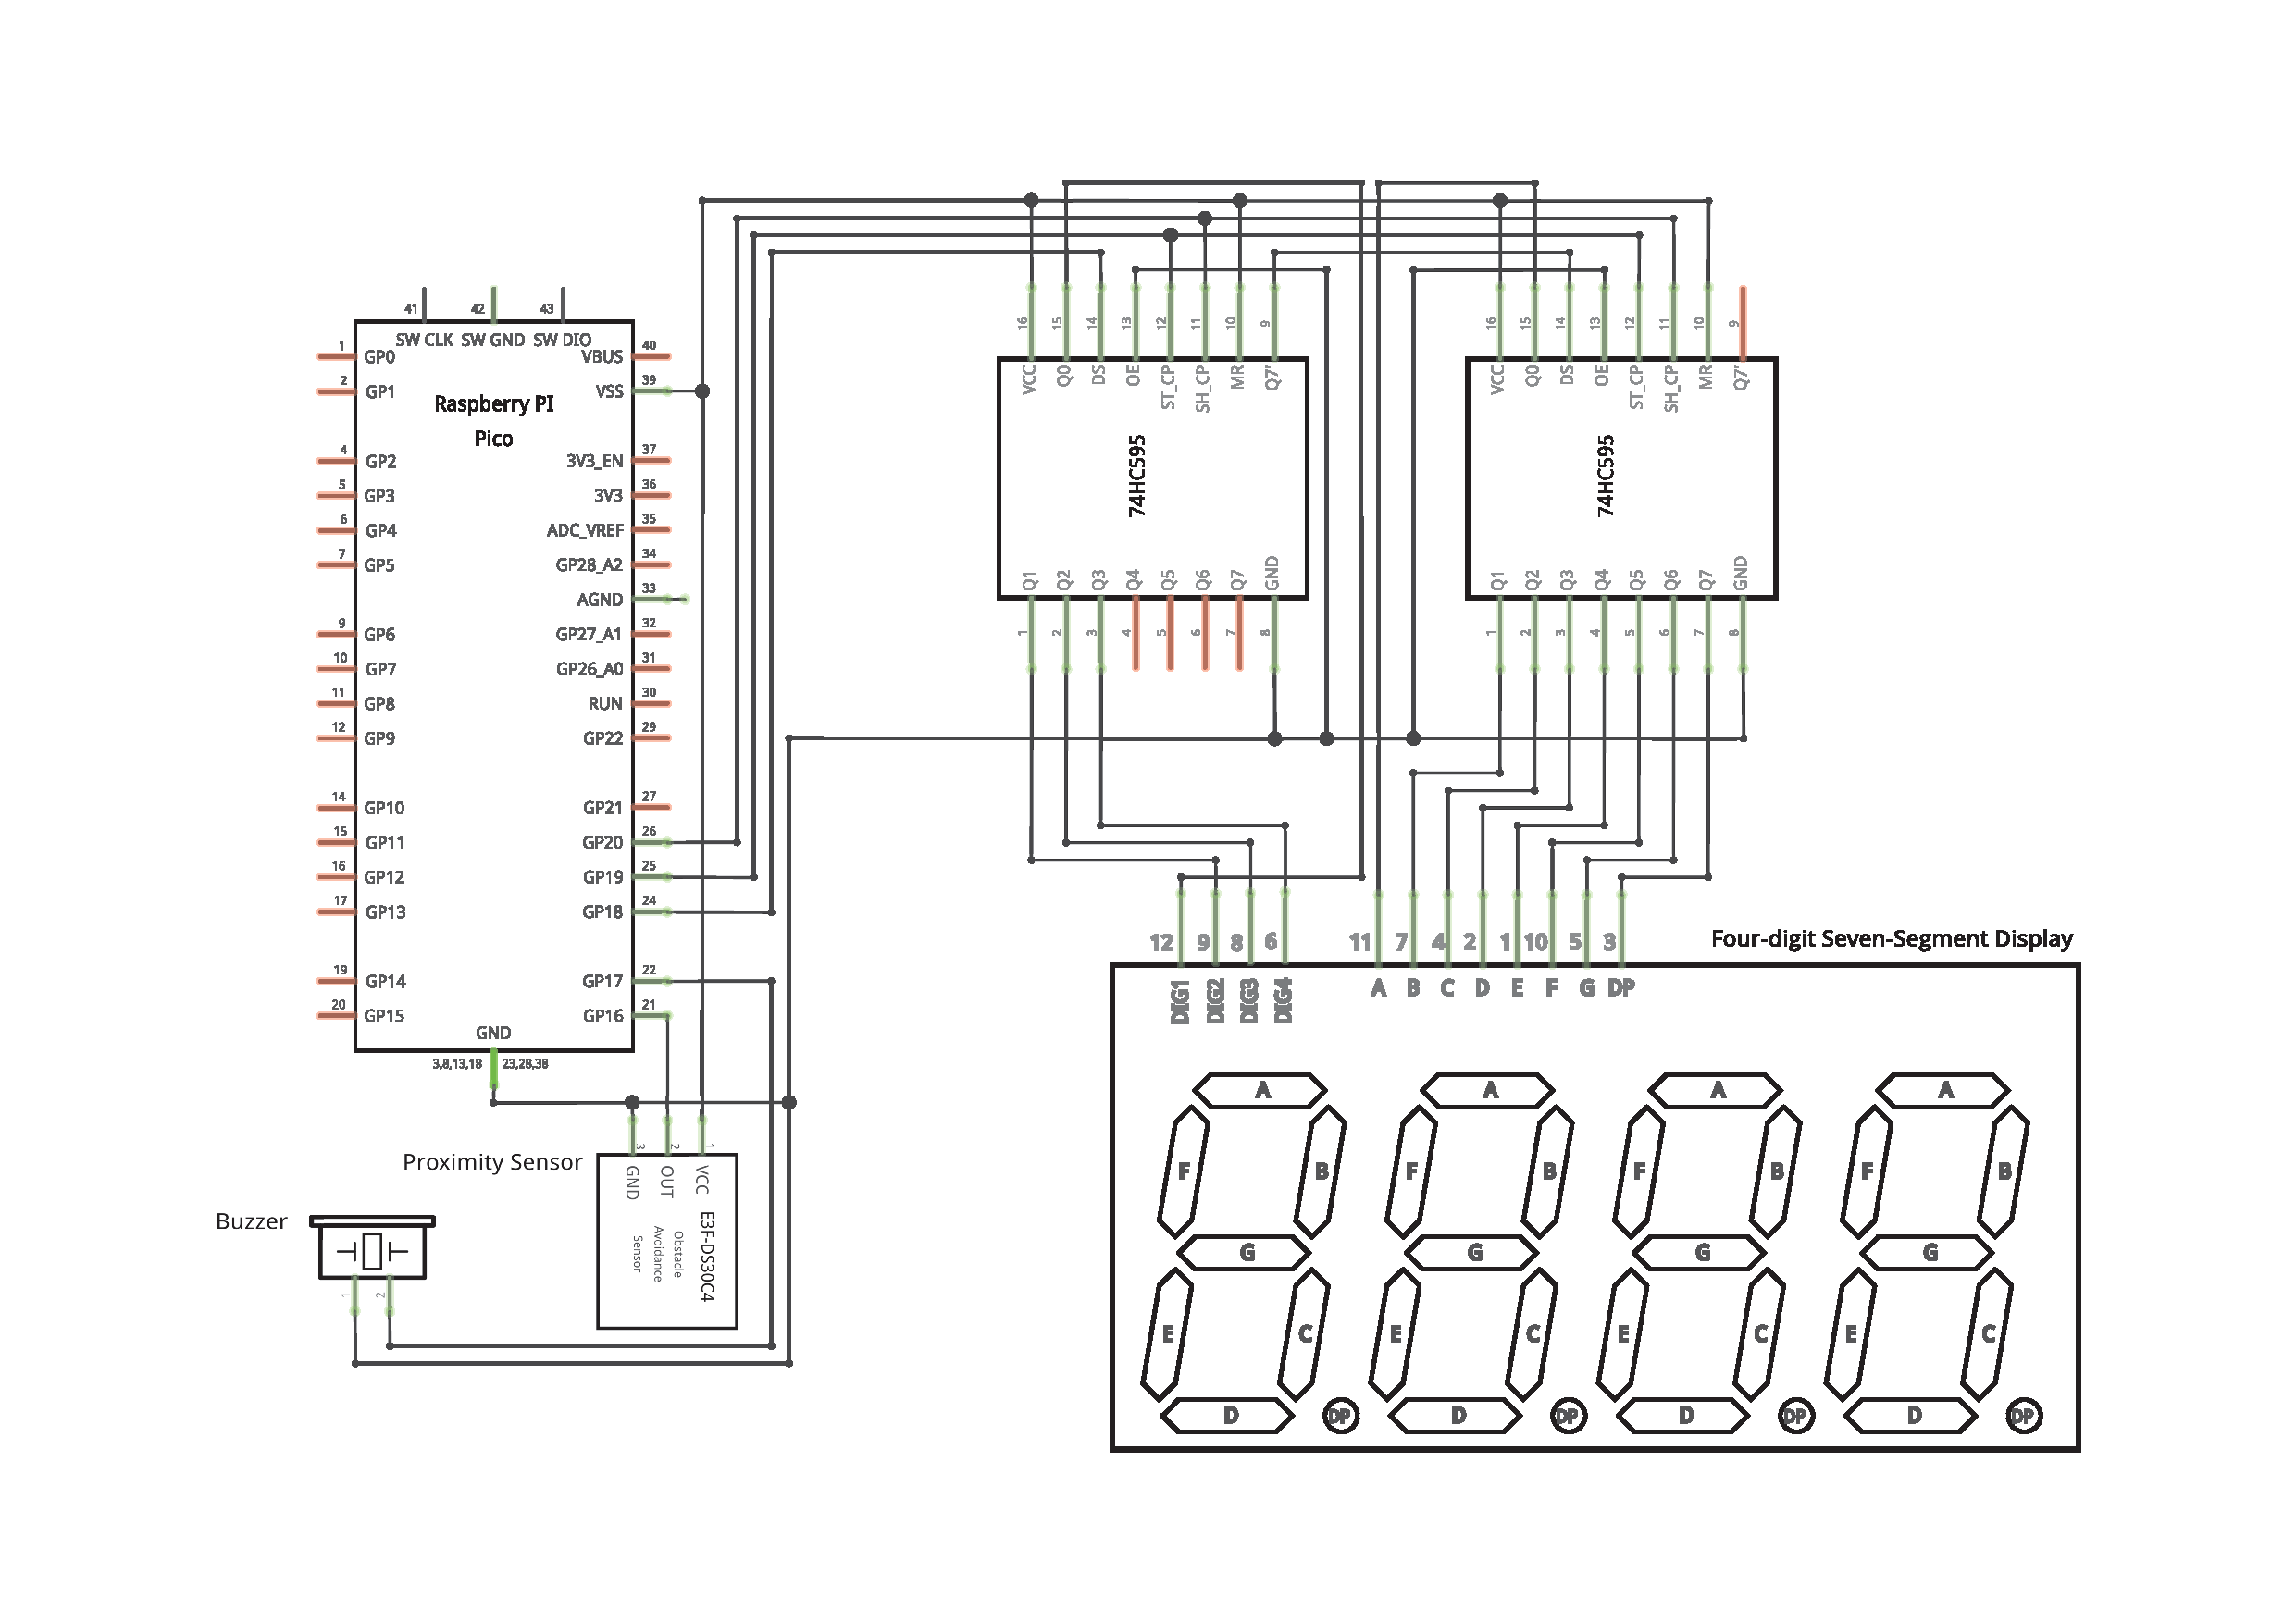
\includepdf[fitpaper,angle=90]{images/wiring_schem_a3.pdf}
\end{landscape}
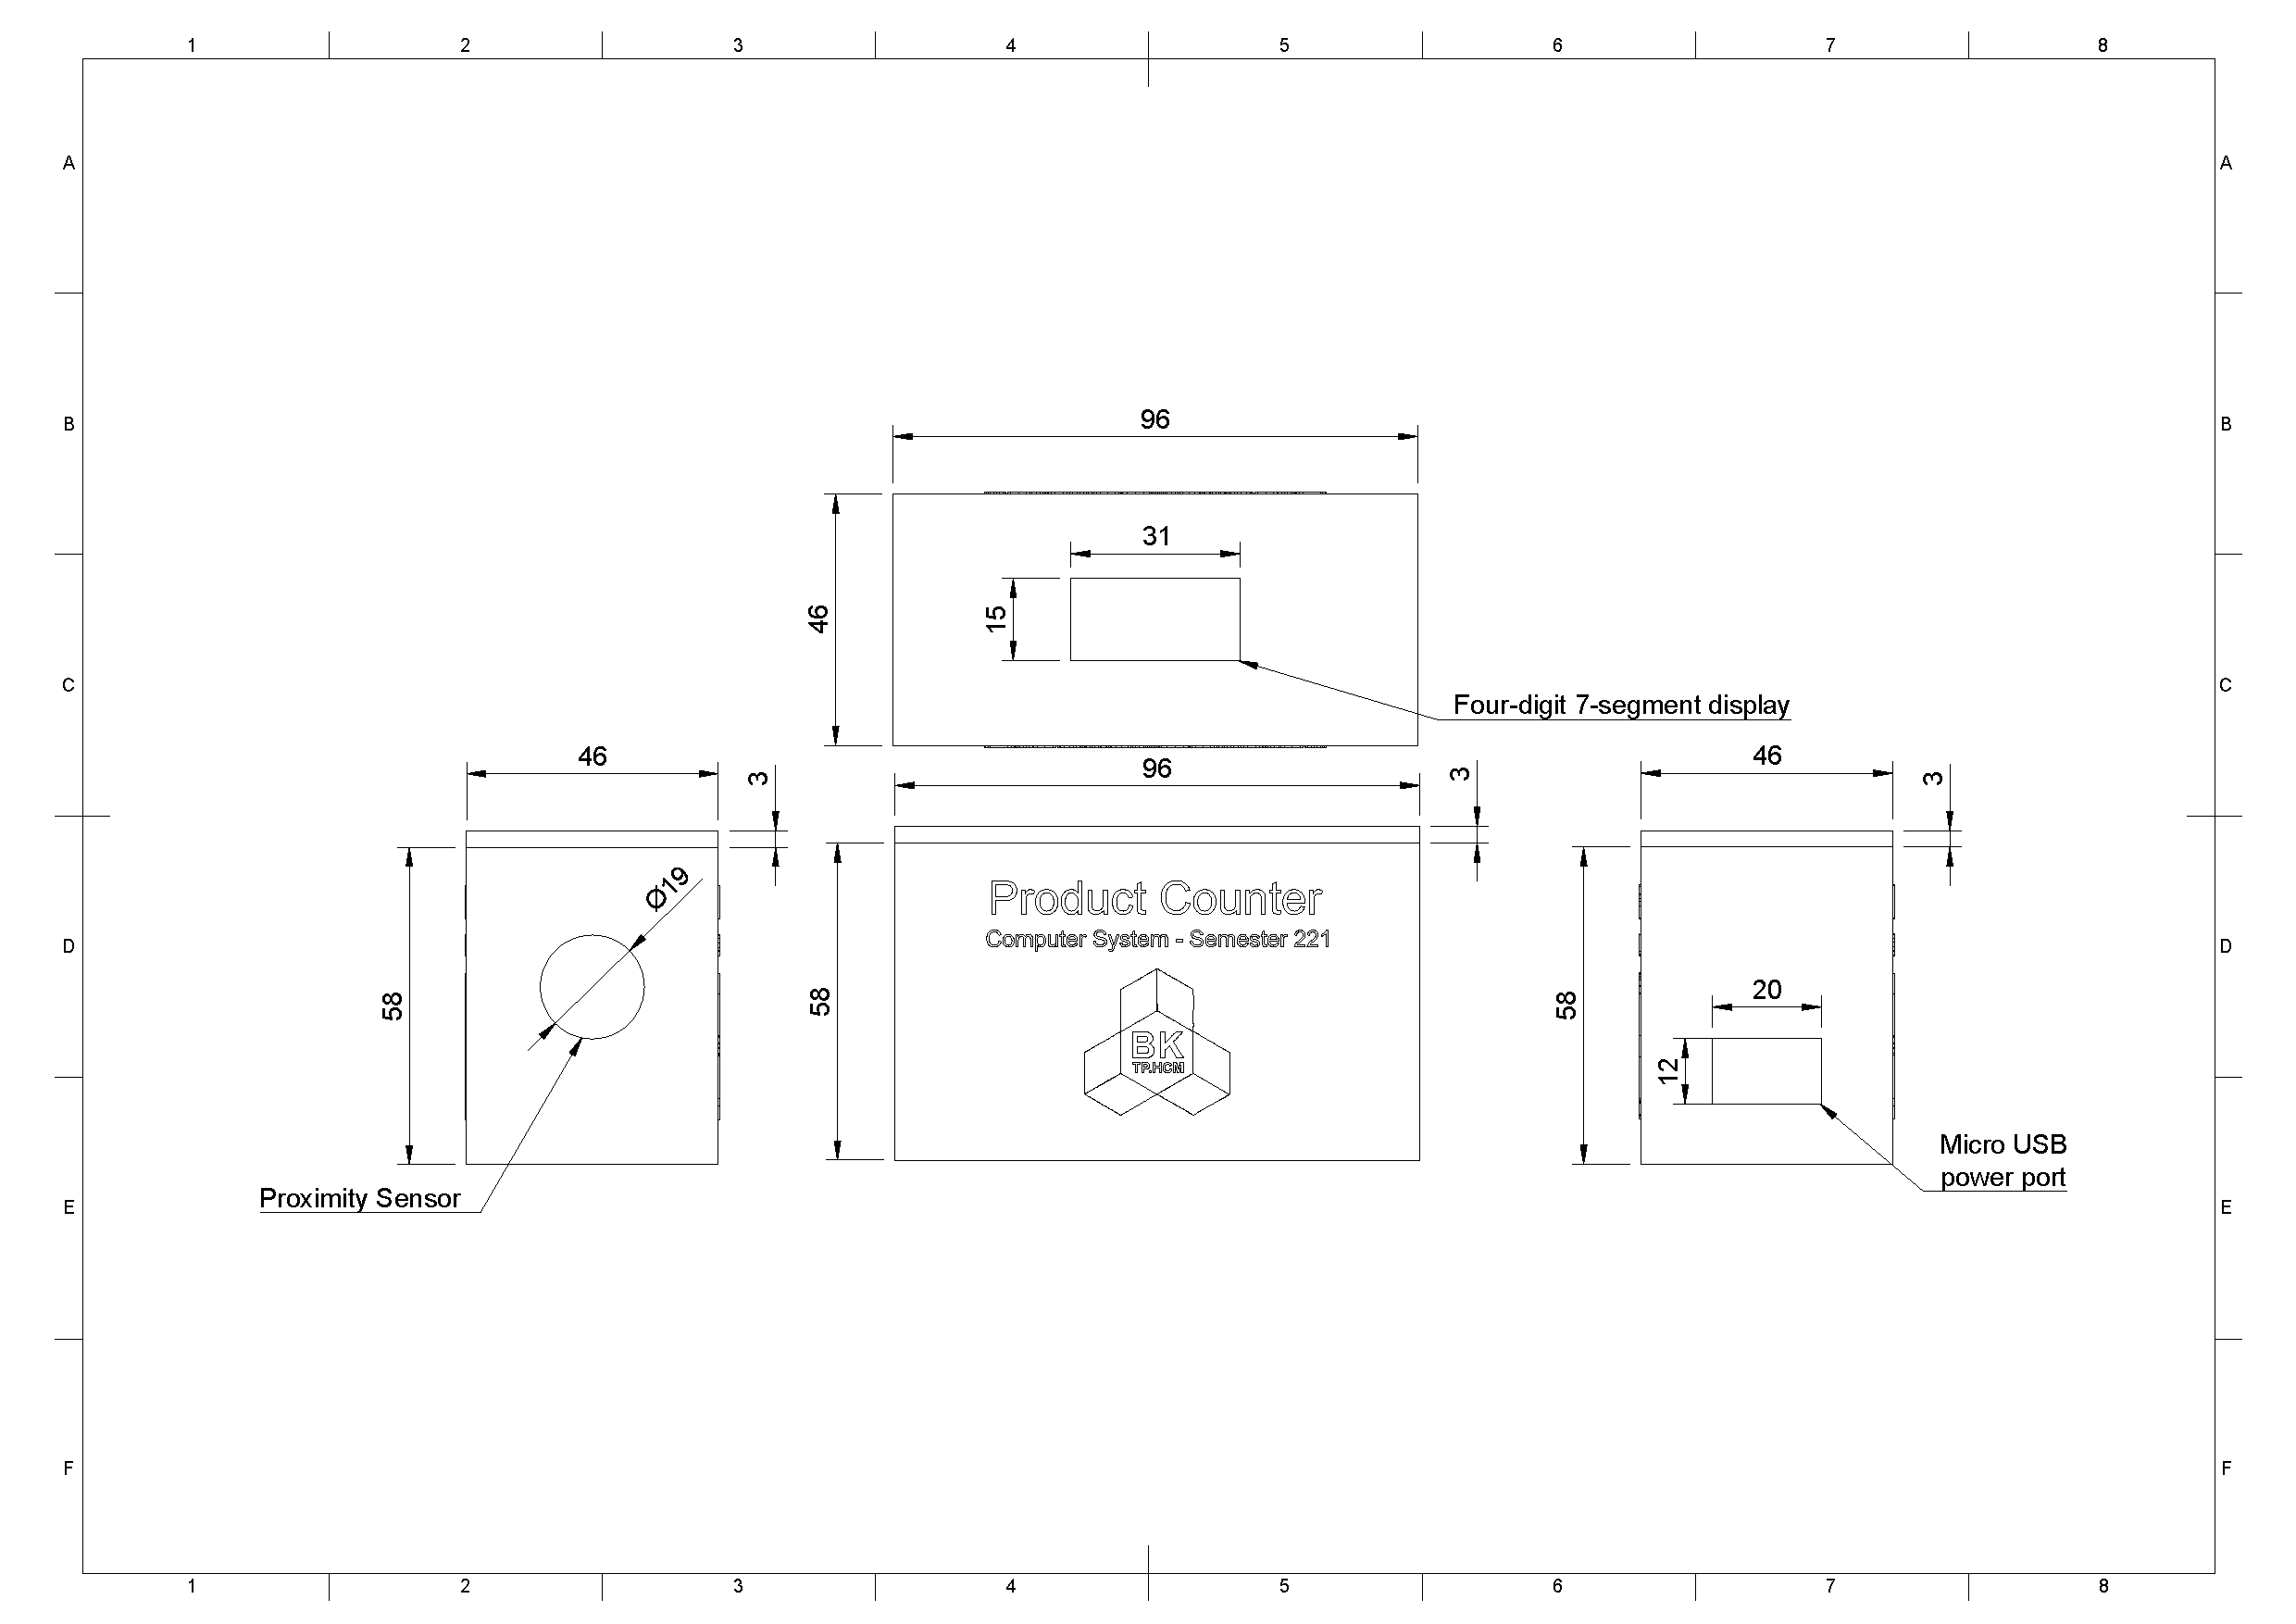
\includepdf[fitpaper]{images/model_schem.pdf}

\end{document}